\documentclass[a4paper,11pt,twoside]{report}
\usepackage[dutch]{babel}
\usepackage[utf8]{inputenc}
\usepackage{amsmath}
\usepackage{amssymb}
\usepackage{graphicx}
\usepackage[margin=2.5cm,headheight=16pt,headsep=12pt,footskip=18pt]{geometry}
\usepackage[colorlinks=true,linkcolor=darkblue,urlcolor=darkblue,citecolor=darkred]{hyperref}
\usepackage{booktabs}
\usepackage{enumitem}
\usepackage{float}
\usepackage{pdfpages}
\usepackage{tikz}
\usepackage{fancyhdr}
\usepackage{xcolor}
\usepackage[stretch=10,expansion=false]{microtype}
\usepackage{soul}
\usepackage[framemethod=tikz]{mdframed}
\usepackage{titlesec}

% ============ TERMINOLOGY AND SYMBOL BOXES ============
\newcommand{\term}[1]{\textbf{#1}}

\newmdenv[
    linewidth=0.6pt,
    roundcorner=4pt,
    linecolor=darkblue,
    backgroundcolor=lightblue,
    innertopmargin=4pt,
    innerbottommargin=4pt,
    innerleftmargin=6pt,
    innerrightmargin=6pt,
    skipabove=6pt,
    skipbelow=6pt
]{symbolbox}

\makeatletter
\newcommand{\SymbolenStromingen}{}
\newcommand{\SymbolenWarmte}{}
\newcommand{\symentryS}[3]{\g@addto@macro\SymbolenStromingen{$#1$ & #2 & #3\\}}
\newcommand{\symentryW}[3]{\g@addto@macro\SymbolenWarmte{$#1$ & #2 & #3\\}}
\newcommand{\symwriteS}[3]{\protected@write\@auxout{}{\string\symentryS{#1}{#2}{#3}}}
\newcommand{\symwriteW}[3]{\protected@write\@auxout{}{\string\symentryW{#1}{#2}{#3}}}
\makeatother

% Symbol introduction helpers:
% - shows a small explanation box the first time
% - registers the symbol once for the formularium (via .aux)
\makeatletter
\newcommand{\sym@key}[1]{\pdfmdfivesum{\detokenize{#1}}}
\newcommand{\symS}[3]{%
    \edef\sym@k{\sym@key{#1}}%
    \ifcsname symS@seen@\sym@k\endcsname
        % already introduced -> do nothing
    \else
        \expandafter\gdef\csname symS@seen@\sym@k\endcsname{}%
        \begin{symbolbox}\textbf{\ensuremath{#1}} --- #2\hfill{\footnotesize\textcolor{gray}{#3}}\end{symbolbox}%
        \symwriteS{#1}{#2}{#3}%
    \fi
}
\newcommand{\symW}[3]{%
    \edef\sym@k{\sym@key{#1}}%
    \ifcsname symW@seen@\sym@k\endcsname
        % already introduced -> do nothing
    \else
        \expandafter\gdef\csname symW@seen@\sym@k\endcsname{}%
        \begin{symbolbox}\textbf{\ensuremath{#1}} --- #2\hfill{\footnotesize\textcolor{gray}{#3}}\end{symbolbox}%
        \symwriteW{#1}{#2}{#3}%
    \fi
}
\makeatother

% ============ COLOR DEFINITIONS ============
\definecolor{darkblue}{RGB}{0,51,102}
\definecolor{lightblue}{RGB}{230,242,255}
\definecolor{darkred}{RGB}{153,0,0}
\definecolor{darkgreen}{RGB}{0,102,51}
\definecolor{gray}{RGB}{80,80,80}
\definecolor{lightgray}{RGB}{240,240,240}

% ============ PAGE HEADERS AND FOOTERS ============
\pagestyle{fancy}
\fancyhf{}
\fancyhead[LE,RO]{\small\bfseries\thepage}
\fancyhead[RE]{\small\nouppercase{\leftmark}}
\fancyhead[LO]{\small\nouppercase{\rightmark}}
\renewcommand{\headrulewidth}{0.4pt}
\renewcommand{\footrulewidth}{0pt}

% ============ CHAPTER AND SECTION STYLING ============
\csname titleformat\endcsname{\chapter}
    {\normalfont\huge\bfseries}
    {\thechapter}
    {1em}
    {}

\csname titleformat\endcsname{\section}
    {\normalfont\Large\bfseries}
    {\thesection}
    {0.8em}
    {}

\csname titleformat\endcsname{\subsection}
    {\normalfont\large\bfseries}
    {\thesubsection}
    {0.8em}
    {}

% Compact vertical spacing around titles
\csname titlespacing\endcsname*{\chapter}{0pt}{1.0ex plus 0.2ex minus 0.2ex}{1.2ex plus 0.2ex}
\csname titlespacing\endcsname*{\section}{0pt}{1.2ex plus 0.2ex minus 0.2ex}{0.8ex plus 0.2ex}
\csname titlespacing\endcsname*{\subsection}{0pt}{1.0ex plus 0.2ex minus 0.2ex}{0.6ex plus 0.2ex}

% ============ DYNAMIC EXERCISE NUMBERING ============
\newcounter{opgave}[section]
\newcommand{\opgave}[1]{%
    \refstepcounter{opgave}%
    \subsection*{\textbf{\arabic{opgave}.} #1}%
}



\title{{\LARGE\textcolor{darkblue}{\textbf{Handboek voor Thermische en Fluïdumwetenschappen}}} \\ \large \textcolor{darkred}{Theorie, Analyse en Toepassingen}}
\author{}
\date{\textcolor{gray}{\today}}

\begin{document}

{\let\newpage\relax\maketitle}

{\textcolor{darkblue}{\tableofcontents}}

\chapter*{Formularium}

\includepdf{Warmte en stroming_Thermal-Fluid Sciences Formularium.pdf}

\addcontentsline{toc}{chapter}{Formularium}
\vspace{-1em}
{\small \textcolor{gray}{Kernformules en een symbolenoverzicht per deel. Nieuwe symbolen noteer je met \term{\textbackslash symS} (stromingen) of \term{\textbackslash symW} (warmte), zodat ze automatisch in de tabellen hieronder terechtkomen (na hercompileren).}}\vspace{0.8em}

\section*{Deel 1: Stromingen}
\subsection*{Belangrijke Formules}
\begingroup
\setlength{\tabcolsep}{6pt}
\renewcommand{\arraystretch}{1.35}
\[
\begin{array}{@{}lcl@{}}
    	\textbf{Dichtheid} &:& \rho=\dfrac{m}{V}\\
    	\textbf{Schuifspanning (Newtoniaans)} &:& \tau=\mu\,\dfrac{\partial u}{\partial y}\\
    	\textbf{Kinematische viscositeit} &:& \nu=\dfrac{\mu}{\rho}\\
    	\textbf{Hydrostatische druk} &:& p=p_0+\rho g h\\
    	\textbf{Continu\"iteit (massadebiet)} &:& \dot{m}=\rho A V\\
    	\textbf{Continu\"iteit (incompressibel)} &:& A_1V_1=A_2V_2\\
        		\textbf{Continu\"iteit (differentieel)} &:& \dfrac{\partial \rho}{\partial t}+\nabla\cdot(\rho\vec{v})=0\\
    	\textbf{Bernoulli (zonder verliezen)} &:& \dfrac{p}{\rho}+\dfrac{V^2}{2}+gz=\text{const.}\\
        		\textbf{Bernoulli (met verliezen)} &:& \dfrac{p_1}{\rho g}+\dfrac{V_1^2}{2g}+z_1=\dfrac{p_2}{\rho g}+\dfrac{V_2^2}{2g}+z_2+h_L\\
        		\textbf{Darcy--Weisbach} &:& h_f=f\,\dfrac{L}{D}\,\dfrac{V^2}{2g}\\
        		\textbf{Kleine verliezen} &:& h_m=K\,\dfrac{V^2}{2g}\\
    	\textbf{Reynoldsgetal} &:& Re=\dfrac{\rho V D}{\mu}=\dfrac{V D}{\nu}\\
\end{array}
\]
\endgroup

% Stromings-symbolen (automatisch aangemaakt bij eerste introductie)
\symS{h_L}{totaal energieverlies (head loss)}{m}
\symS{h_f}{wrijvingskopverlies}{m}
\symS{f}{wrijvingsfactor (Darcy)}{-}
\symS{K}{verliescoëfficiënt}{-}
\symS{\varepsilon}{absolute wandruwheid}{m}

\subsection*{Grootheden en symbolen}
\begingroup
\setlength{\tabcolsep}{6pt}
\renewcommand{\arraystretch}{1.25}
\begin{tabular}{@{}lll@{}}
\toprule
Symbool & Betekenis & Eenheid\\
\midrule
\SymbolenStromingen
\bottomrule
\end{tabular}
\endgroup

\section*{Deel 2: Warmte}
\subsection*{Belangrijke Formules}
\begingroup
\setlength{\tabcolsep}{6pt}
\renewcommand{\arraystretch}{1.35}
\[
\begin{array}{@{}lcl@{}}
    	\textbf{Eerste hoofdwet (gesloten)} &:& \Delta U=Q-W\\
    	\textbf{Eerste hoofdwet (stationair CV)} &:& \dot{Q}-\dot{W}=\sum\dot{m}\left(h+\dfrac{V^2}{2}+gz\right)_{out}-\sum\dot{m}\left(h+\dfrac{V^2}{2}+gz\right)_{in}\\
    		\textbf{Enthalpie} &:& h=u+pv\\
    	\textbf{Ideaal gas} &:& p v = R T\\
    	\textbf{Clausius-ongelijkheid} &:& \Delta S\ge\displaystyle\int\frac{\delta Q}{T}\\
    	\textbf{Entropiebalans (stationair CV)} &:& \dot{S}_{gen}=\sum\dot{m}\,s_{out}-\sum\dot{m}\,s_{in}-\sum\dfrac{\dot{Q}_k}{T_k}\\
    	\textbf{Fourier (1D)} &:& \dot{Q}=-kA\,\dfrac{dT}{dx}\\
    	\textbf{Convectie (Newton)} &:& \dot{Q}=hA\,(T_s-T_\infty)\\
    	\textbf{Straling (Stefan--Boltzmann)} &:& \dot{Q}=\varepsilon\sigma A\,(T_s^4-T_\infty^4)\\
    		\textbf{Warmtewisselaar (LMTD)} &:& \dot{Q}=UA\,\Delta T_{lm}\\
\end{array}
\]
\symW{k}{thermische geleidbaarheid}{$W/(m\,K)$}
\symW{U}{globale warmteoverdrachtscoëfficiënt}{$W/(m^2\,K)$}
\symW{\varepsilon}{emissiviteit}{-}
\symW{\sigma}{Stefan--Boltzmann constante}{$W/(m^2\,K^4)$}
\begin{tabular}{@{}lll@{}}
\toprule
Symbool & Betekenis & Eenheid\\
\midrule
\SymbolenWarmte
\bottomrule
\end{tabular}
\endgroup

\clearpage


\chapter*{Inleiding}
\vspace{-1em}
{\small \textcolor{gray}{Dit handboek behandelt de kernprincipes van thermodynamica, fluïdummechanica en warmteoverdracht.}}\vspace{1em}

In de wereld van de ingenieurswetenschappen vormen de disciplines thermodynamica, fluïdummechanica en warmteoverdracht de fundamentele bouwstenen voor het begrijpen van energie en materie. Deze vakgebieden, vaak gezamenlijk aangeduid als de \textcolor{darkblue}{\textbf{thermische en fluïdumwetenschappen}}, zijn onlosmakelijk met elkaar verbonden. Of het nu gaat om het ontwerpen van een straalmotor, het optimaliseren van een warmtewisselaar in een energiecentrale, of het modelleren van bloedstroom in het menselijk lichaam, de interactie tussen thermische energie en stromende media speelt een centrale rol.

Dit rapport biedt een uitputtende analyse van deze wetenschappen, gebaseerd op een synthese van academische bronteksten, vraagstukken en handboeken. Het document is gestructureerd in drie hoofddelen: \textcolor{darkblue}{\textbf{Deel 1: Stromingen}}, dat de mechanica van vloeistoffen en gassen in rust en beweging behandelt; \textcolor{darkblue}{\textbf{Deel 2: Warmte}}, waarin de wetten van de thermodynamica en warmteoverdracht worden ontleed; en \textcolor{darkblue}{\textbf{Deel 3: Oefeningen}}, waarin de theorie wordt toegepast op concrete technische vraagstukken. De benadering is gericht op een stap-voor-stap uitleg van concepten en formules, waarbij complexe fysische fenomenen worden vertaald naar begrijpelijke en toepasbare kennis.

\part{Stromingen}

\chapter{Eigenschappen van Fluïda}
\section{Definitie van een Fluïdum}
Een \term{fluïdum} is een stof die niet in staat is blijvende weerstand te bieden tegen afschuiving. Waar een vaste stof zijn vorm behoudt onder schuifspanning, zal een fluïdum continu blijven vervormen zolang de schuifkracht wordt aangehouden. Fluïda omvatten zowel vloeistoffen als gassen.

\section{Dichtheid}
De dichtheid $\rho$ van een fluïdum wordt gedefinieerd als de massa per volume-eenheid:
\[
\rho = \frac{m}{V} \quad [kg/m^3]
\]
\symS{\rho}{dichtheid}{kg/m$^3$}
\symS{m}{massa}{kg}
Voor een continuum-benadering is er een minimum volume $V^*$ nodig waaronder de dichtheid constant blijft. Voor water geldt bijvoorbeeld dat $1 \, mm^3 \approx 3 \times 10^{16}$ moleculen bevat, waardoor de continuum-aanname gerechtvaardigd is.

\section{Viscositeit}
Viscositeit is een maat voor de interne wrijving van een fluïdum. Voor een Newtoniaans fluïdum geldt een lineair verband tussen de schuifspanning $\tau$ en de snelheidsgradiënt:
\[
\tau = \mu \frac{\partial u}{\partial y}
\]
\symS{\tau}{schuifspanning}{Pa}
\symS{\mu}{dynamische viscositeit}{Pa\,s}
waarbij:
\begin{itemize}
    \item $\tau$ de schuifspanning is [Pa]
    \item $\mu$ de dynamische viscositeit [Pa·s]
    \item $\frac{\partial u}{\partial y}$ de snelheidsgradiënt loodrecht op de stroomrichting
\end{itemize}
De kinematische viscositeit wordt gedefinieerd als:
\[
\nu = \frac{\mu}{\rho} \quad [m^2/s]
\]
\symS{\nu}{kinematische viscositeit}{m$^2$/s}
Voor vloeistoffen neemt de viscositeit af met toenemende temperatuur, terwijl voor gassen de viscositeit toeneemt met temperatuur.

\subsubsection*{Voorbeeld: Schuifspanning in een olielaag}
\textbf{Gegeven:} Een vlakke plaat met oppervlakte $A = 0.5 \, m^2$ wordt met een snelheid van $V = 2 \, m/s$ over een vlakke ondergrond getrokken. Tussen de plaat en de ondergrond bevindt zich een olielaagje met dikte $d = 1 \, mm$ en dynamische viscositeit $\mu = 0.1 \, Pa \cdot s$.
\symS{A}{oppervlakte}{m$^2$}
\symS{V}{snelheid}{m/s}
\symS{d}{laagdikte}{m}
\textbf{Gevraagd:} Bereken de benodigde kracht $F$ om de plaat te bewegen.
\symS{F}{kracht}{N}
\textbf{Oplossing:}
De snelheidsgradiënt is lineair (Couette stroming):
\[
\frac{du}{dy} \approx \frac{V}{d} = \frac{2 \, m/s}{0.001 \, m} = 2000 \, s^{-1}
\]
De schuifspanning is:
\[
\tau = \mu \frac{du}{dy} = 0.1 \cdot 2000 = 200 \, Pa
\]
De benodigde kracht is:
\[
F = \tau \cdot A = 200 \, N/m^2 \cdot 0.5 \, m^2 = 100 \, N
\]

\begin{figure}[H]
    \centering
    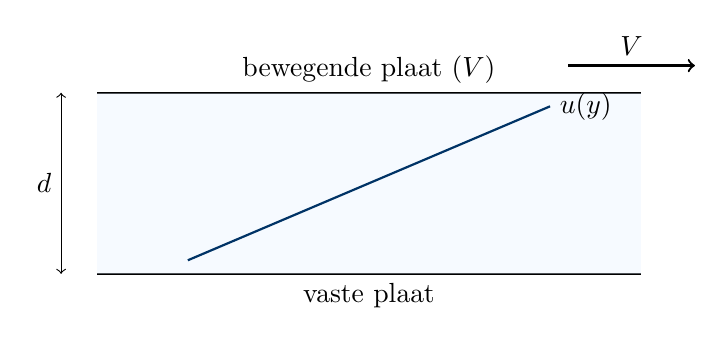
\begin{tikzpicture}[x=1.15cm,y=1.15cm]
        % plates
        \draw[thick] (0,0) -- (6,0);
        \draw[thick] (0,2) -- (6,2);
        \node[below] at (3,0) {vaste plaat};
        \node[above] at (3,2) {bewegende plaat ($V$)};

        % fluid region
        \fill[lightblue,opacity=0.35] (0,0) rectangle (6,2);

        % velocity profile
        \draw[thick,darkblue] (1.0,0.15) -- (5.0,1.85);
        \node[right] at (5.0,1.85) {$u(y)$};

        % arrow for plate motion
        \draw[thick,->] (5.2,2.3) -- (6.6,2.3);
        \node[above] at (5.9,2.3) {$V$};

        % gap label
        \draw[<->] (-0.4,0) -- (-0.4,2);
        \node[left] at (-0.4,1) {$d$};
    \end{tikzpicture}
    \caption{Couette-stroming: lineair snelheidsprofiel tussen een vaste en een bewegende plaat.}
\end{figure}

\chapter{Fluïdumstatica (Hydrostatica)}
Fluïdumstatica behandelt vloeistoffen die in rust zijn. In deze toestand zijn er geen relatieve bewegingen tussen vloeistoflagen, dus er zijn geen schuifspanningen. Alleen normaalkrachten (druk) spelen een rol.

\section{Drukverdeling in een Fluïdum in Rust}
\subsection{Het Infinitesimale Controle Volume}
We beginnen met het beschouwen van een infinitesimaal klein controle volume in een fluïdum dat in rust is. Dit is een kubisch volume met afmetingen:
\begin{itemize}
    \item Lengte in x-richting: $dx$
    \item Lengte in y-richting: $dy$
    \item Lengte in z-richting: $dz$
\end{itemize}
Het volume van dit element is dus:
\[
dV = dx \cdot dy \cdot dz
\]
\textbf{Belangrijke aanname:} Het fluïdum is in rust, wat betekent dat er geen weerstand tegen schuifspanningen optreedt in het fluïdum. De enige krachten die werken zijn drukkrachten (loodrecht op oppervlakken) en zwaartekrachten.

\subsection{Identificatie van Krachten}
Op dit controle volume werken verschillende krachten:

\textbf{1. Drukkrachten op elk oppervlak:}
\begin{itemize}
    \item \textbf{Linkervlak (in x-richting):}
    \begin{itemize}
        \item Oppervlakte: $A_x = dy \cdot dz$
        \item Druk: $p$
        \item Kracht richting positieve x: $F_{x,links} = p \cdot dy \cdot dz$
    \end{itemize}
    \item \textbf{Rechtervlak (in x-richting):}
    \begin{itemize}
        \item Oppervlakte: $A_x = dy \cdot dz$
        \item Druk: $p + \frac{\partial p}{\partial x} dx$ (druk verandert over afstand $dx$)
        \item Kracht richting negatieve x: $F_{x,rechts} = -\left(p + \frac{\partial p}{\partial x} dx\right) \cdot dy \cdot dz$
    \end{itemize}
\end{itemize}

\symS{p}{druk}{Pa}

\textbf{2. Zwaartekracht:}
De massa van het element is:
\[
dm = \rho \cdot dV = \rho \cdot dx \cdot dy \cdot dz
\]
De zwaartekracht werkt in de negatieve z-richting:
\[
G = dm \cdot g = \rho \cdot g \cdot dx \cdot dy \cdot dz
\]

\symS{g}{zwaartekrachtsversnelling}{m/s$^2$}

\subsection{Krachtenevenwicht}
\textbf{Krachtenevenwicht in x-richting:}
Voor een fluïdum in rust moet de som van alle krachten in x-richting nul zijn ($\sum F_x = 0$):
\[
p \cdot dy \cdot dz - \left(p + \frac{\partial p}{\partial x} dx\right) \cdot dy \cdot dz = 0
\]
Uitwerken:
\[
-\frac{\partial p}{\partial x} dx \cdot dy \cdot dz = 0 \implies \frac{\partial p}{\partial x} = 0
\]
\textbf{Conclusie:} De druk verandert niet in de horizontale x-richting in een fluïdum in rust.

\textbf{Krachtenevenwicht in y-richting:}
Volledig analoog aan de x-richting ($\sum F_y = 0$):
\[
\frac{\partial p}{\partial y} = 0
\]
\textbf{Conclusie:} De druk verandert niet in de horizontale y-richting in een fluïdum in rust.

\textbf{Krachtenevenwicht in z-richting (verticaal):}
In de verticale richting hebben we zowel drukkrachten als zwaartekracht.
\begin{itemize}
    \item \textbf{Ondervlak (beneden):} Kracht omhoog $F_{z,onder} = p \cdot dx \cdot dy$
    \item \textbf{Bovenvlak (boven):} Kracht omlaag $F_{z,boven} = -\left(p + \frac{\partial p}{\partial z} dz\right) \cdot dx \cdot dy$
    \item \textbf{Zwaartekracht:} Omlaag $G = -\rho g \cdot dx \cdot dy \cdot dz$
\end{itemize}
Krachtenevenwicht ($\sum F_z = 0$):
\[
p \cdot dx \cdot dy - \left(p + \frac{\partial p}{\partial z} dz\right) \cdot dx \cdot dy - \rho g \cdot dx \cdot dy \cdot dz = 0
\]
Uitwerken en delen door $dx \cdot dy \cdot dz$:
\[
-\frac{\partial p}{\partial z} - \rho g = 0 \implies \frac{\partial p}{\partial z} = -\rho g
\]
\textbf{Cruciale conclusie:} De druk neemt af in de positieve z-richting (omhoog). Dit betekent dat de druk toeneemt met de diepte!

\subsection{Integratie}
\textbf{Integratie voor Vloeistoffen ($\rho = \text{constant}$):}
\[
\int_{z_1}^{z_2} dp = \int_{z_1}^{z_2} (-\rho g) \, dz \implies p_2 - p_1 = -\rho g (z_2 - z_1)
\]
Als we definiëren dat $h = z_1 - z_2$ (de diepte onder punt 1):
\[
p_2 = p_1 + \rho g h
\]
Dit is de fundamentele hydrostatische vergelijking. Voor water ($\rho \approx 1000 \, kg/m^3$) is $\Delta p \approx 9810 \, Pa/m \approx 0.1 \, bar/m$.

\textbf{Integratie voor Gassen ($\rho = \rho(z)$):}
Voor gassen volgt de dichtheid de ideale gaswet $\rho = \frac{p}{RT}$. Substitueren in $\frac{dp}{dz} = -\rho g$:
\[
\frac{dp}{dz} = -\frac{p \cdot g}{RT} \implies \frac{dp}{p} = -\frac{g}{RT} dz
\]
Voor een isotherme atmosfeer ($T = \text{constant}$), integreren van $z_1$ tot $z_2$:
\[
p_2 = p_1 \exp\left(-\frac{g(z_2 - z_1)}{RT}\right)
\]
Dit verklaart waarom de luchtdruk exponentieel afneemt met de hoogte.

\subsubsection*{Voorbeeld: Druk op diepte}
\textbf{Gegeven:} Een duiker bevindt zich op $20 \, m$ diepte in zeewater ($\rho = 1025 \, kg/m^3$). De atmosferische druk aan het oppervlak is $P_{atm} = 101.3 \, kPa$.
\textbf{Gevraagd:} De absolute druk op de duiker.
\textbf{Oplossing:}
\[
P = P_{atm} + \rho g h
\]
\[
P = 101300 + 1025 \cdot 9.81 \cdot 20
\]
\[
P = 101300 + 201105 = 302405 \, Pa \approx 3.02 \, bar
\]

\begin{figure}[H]
    \centering
    \includegraphics[width=0.4\textwidth]{assets/hydrostatic_pressure.jpg}
    \caption{Lineaire toename van hydrostatische druk met de diepte.}
    \label{fig:hydrostatic_pressure}
\end{figure}

\begin{figure}[H]
    \centering
    \includegraphics[width=0.2\textwidth]{assets/wikipedia/manometer_utube_pd_500.png}
    \caption{U-buis manometer (schematisch).\;\scriptsize Bron: Mintz l, publiek domein, via Wikimedia Commons (\url{https://commons.wikimedia.org/wiki/File:Manometer_(schematic_U-tube).svg}).}
\end{figure}

\subsubsection*{Voorbeeldoefening: manometer (drukverschil)}
                        	\textbf{Gegeven:} Een U-buis manometer met kwik ($\rho_{Hg}=13\,600\,\mathrm{kg/m^3}$) toont een niveauverschil $h=12\,\mathrm{cm}$.\\
                        	\textbf{Gevraagd:} Bepaal $\Delta p=p_{tank}-p_{atm}$.\\
                        	\textbf{Oplossing:}
\[
\Delta p=\rho g h=13\,600\cdot 9.81\cdot 0.12\approx 1.60\times 10^4\,\mathrm{Pa}=16.0\,\mathrm{kPa}
\]

\section{Krachten op Onderdompelde Oppervlakken}
\subsection{Rechthoekig Oppervlak - Basisprobleem}
Beschouw een rechthoekig oppervlak volledig ondergedompeld in water:
\begin{itemize}
    \item Breedte: $b$
    \item Hoogte: $a$
    \item Georiënteerd verticaal ($\theta = 90^\circ$)
    \item Bovenkant op diepte 0, onderkant op diepte $a$
\end{itemize}

\textbf{Drukverdeling en Totale Kracht:}
Op diepte $y$ is de druk $p(y) = \rho g y$ (waarbij $p_0$ verwaarloosbaar is).
De kracht op een infinitesimale strip met hoogte $dy$ is $dF = p(y) \cdot b \cdot dy = \rho g y \cdot b \cdot dy$.
Integreren over de hoogte:
\[
F = \int_0^a \rho g y \cdot b \, dy = \rho g b \left[ \frac{y^2}{2} \right]_0^a = \frac{1}{2} \rho g b a^2
\]
Alternatief: $F = p_{gem} \cdot A = (\rho g \frac{a}{2}) \cdot (ab) = \frac{1}{2} \rho g a^2 b$.

\textbf{Aangrijpingspunt (Center of Pressure):}
Het moment van de drukkracht om de bovenkant moet gelijk zijn aan het moment van de resulterende kracht ($F \cdot y_p = \int y \cdot dF$):
\[
F \cdot y_p = \int_0^a y \cdot (\rho g y \cdot b) \, dy = \rho g b \int_0^a y^2 \, dy = \rho g b \left[ \frac{y^3}{3} \right]_0^a = \frac{1}{3} \rho g b a^3
\]
Invullen van $F$:
\[
\left(\frac{1}{2} \rho g b a^2\right) \cdot y_p = \frac{1}{3} \rho g b a^3 \implies y_p = \frac{2}{3} a
\]
\textbf{Conclusie:} Het aangrijpingspunt ligt op twee derde van de hoogte vanaf de bovenkant.

\subsection{Schuin Rechthoekig Oppervlak onder Hoek \texorpdfstring{$\theta$}{theta}}
\textbf{Coördinatensysteem:}
Voor een oppervlak onder hoek $\theta$ met de horizontaal definiëren we $y'$ als de afstand langs het schuine oppervlak vanaf de bovenkant. De verticale diepte is $h = y' \sin \theta$.

\textbf{Totale Kracht:}
De druk op positie $y'$ is $p(y') = \rho g y' \sin \theta$.
De kracht op een strip is $dF = \rho g y' \sin \theta \cdot b \cdot dy'$.
\[
F = \int_0^a \rho g \sin \theta \cdot b \cdot y' \, dy' = \frac{1}{2} \rho g \sin \theta \cdot b \cdot a^2
\]
De kracht kan ontbonden worden in een horizontale component $F_x = F \sin \theta$ en een verticale component $F_y = F \cos \theta$.

\textbf{Aangrijpingspunt:}
\[
F \cdot y_p = \int_0^a y' \cdot dF = \int_0^a y' \cdot (\rho g \sin \theta \cdot b \cdot y') \, dy' = \frac{1}{3} \rho g \sin \theta \cdot b \cdot a^3
\]
Dit leidt opnieuw tot:
\[
y_p = \frac{2a}{3}
\]

\subsection{Algemene Formules}
\textbf{Totale Kracht:}
Voor een algemeen ondergedompeld oppervlak:
\[
F = p_{gem} \cdot A = (\rho g h_c) \cdot A
\]
waarbij $h_c$ de verticale diepte van het zwaartepunt is.

\textbf{Aangrijpingspunt (Center of Pressure):}
Het aangrijpingspunt wordt bepaald door het traagheidsmoment:
\[\
y_p = y_c + \frac{I_{xx,c}}{y_c \cdot A}
\]
waarbij $y_p$ en $y_c$ posities langs het oppervlak zijn, en $I_{xx,c}$ het traagheidsmoment rond de horizontale as door het zwaartepunt is.

\subsubsection*{Voorbeeld: Kracht op een sluisdeur}
\textbf{Gegeven:} Een rechthoekige sluisdeur is $4 \, m$ breed en het water staat $3 \, m$ hoog tegen de deur.
\textbf{Gevraagd:} De totale hydrostatische kracht op de deur.
\textbf{Oplossing:}
Het zwaartepunt van het natte oppervlak ligt op halve hoogte: $h_c = 1.5 \, m$.
De oppervlakte is $A = 4 \cdot 3 = 12 \, m^2$.
\[
F = \rho g h_c A = 1000 \cdot 9.81 \cdot 1.5 \cdot 12
\]
\[
F = 176580 \, N \approx 176.6 \, kN
\]

\begin{figure}[H]
    \centering
    \includegraphics[width=0.8\textwidth]{assets/submerged_plane.png}
    \caption{Hydrostatische krachten op een ondergedompeld vlak oppervlak.}
    \label{fig:submerged_plane}
\end{figure}

\section{Archimedes' kracht en Drijfvermogen}
Het principe van Archimedes stelt dat een ondergedompeld lichaam een opwaartse kracht ondervindt die gelijk is aan het gewicht van de verplaatste vloeistof:
\[
F_B = \rho_{vloeistof} g V_{ondergedompeld}
\]

\subsection*{Afleiding voor een rechthoekig blok}
Beschouw een rechthoekig blok dat volledig is ondergedompeld in een vloeistof met dichtheid $\rho$. Het blok heeft een boven- en ondervlak met oppervlakte $A$, en hoogte $h$.
De druk in een vloeistof neemt toe met de diepte volgens de hydrostatische wet $p = p_{atm} + \rho g z$.

\begin{itemize}
    \item De druk op het bovenvlak (op diepte $h_1$) is $p_1 = p_{atm} + \rho g h_1$.
    \item De druk op het ondervlak (op diepte $h_2 = h_1 + h$) is $p_2 = p_{atm} + \rho g h_2$.
\end{itemize}

De krachten op de verticale zijwanden heffen elkaar op vanwege symmetrie. De netto verticale kracht wordt bepaald door het drukverschil tussen onder- en bovenkant (waarbij de kracht op de onderkant omhoog werkt en op de bovenkant omlaag):
\begin{align*}
    F_{B} &= F_{onder} - F_{boven} \\
    &= p_2 A - p_1 A \\
    &= (p_{atm} + \rho g h_2) A - (p_{atm} + \rho g h_1) A \\
    &= \rho g (h_2 - h_1) A \\
    &= \rho g h A
\end{align*}
Omdat $V = h \cdot A$ het volume van het blok is, volgt hieruit:
\[
F_B = \rho g V
\]
Dit bevestigt dat de opwaartse kracht gelijk is aan het gewicht van de verplaatste vloeistof.
Deze kracht grijpt aan in het drukkpunt van de verplaatste vloeistof. Voor de stabiliteit van drijvende lichamen is de positie van het metacentrum ten opzichte van het zwaartepunt cruciaal. Als het metacentrum boven het zwaartepunt ligt, ontstaat bij een kleine kanteling een herstellend moment en is het lichaam stabiel.

\begin{figure}[H]
    \centering
    \includegraphics[width=0.3\textwidth]{assets/wikipedia/buoyancy_cc_by_sa_960.png}
    \caption{Drijfvermogen: opwaartse kracht werkt in het drukkingspunt (centrum van opwaartse kracht).\;\scriptsize Bron: Original Yupi666, vector Pbrks, CC BY-SA 3.0, via Wikimedia Commons (\url{https://commons.wikimedia.org/wiki/File:Buoyancy.svg}).}
\end{figure}

\subsubsection*{Voorbeeldoefening: drijfhoogte bepalen}
                	\textbf{Gegeven:} Een houten blok met dichtheid $\rho_{blok}=650\,\mathrm{kg/m^3}$ drijft in water ($\rho_{w}=1000\,\mathrm{kg/m^3}$).\\
                	\textbf{Gevraagd:} Welk deel van het volume is ondergedompeld?\\
                	\textbf{Oplossing:}
In evenwicht: $\rho_w g V_{onder}=\rho_{blok} g V_{totaal}$. Dus:
\[
\frac{V_{onder}}{V_{totaal}}=\frac{\rho_{blok}}{\rho_w}=\frac{650}{1000}=0.65
\]
Dus het blok is voor \boxed{65\%} ondergedompeld.

\chapter{Kinematica van Stromingen}
\section{Euleriaanse Beschrijving}
Er bestaan twee fundamentele benaderingen voor het beschrijven van stromingen:
\begin{itemize}
    \item \textbf{Euleriaanse beschrijving:} We beschrijven het snelheidsveld op vaste punten in de ruimte: $\vec{V}(\vec{x}, t)$.
\end{itemize}

\symS{\vec{v}}{snelheidsvector}{m/s}
\symS{\vec{a}}{versnellingsvector}{m/s$^2$}

\begin{figure}[H]
    \centering
    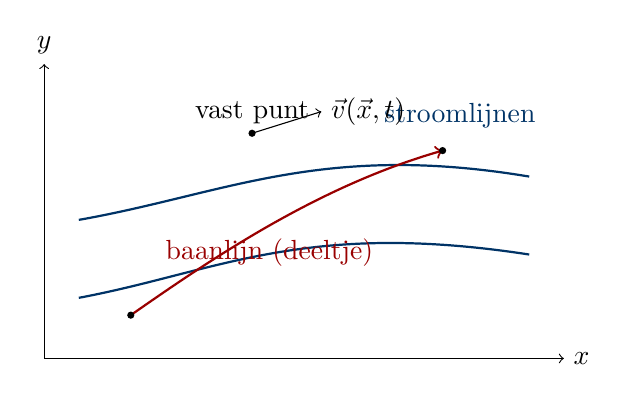
\begin{tikzpicture}[x=1.1cm,y=1.1cm]
        % coordinate frame
        \draw[->] (0,0) -- (6,0) node[right] {$x$};
        \draw[->] (0,0) -- (0,3.4) node[above] {$y$};

        % streamlines
        \draw[thick,darkblue] (0.4,0.7) .. controls (2.0,1.0) and (3.0,1.6) .. (5.6,1.2);
        \draw[thick,darkblue] (0.4,1.6) .. controls (2.1,1.9) and (3.2,2.5) .. (5.6,2.1);
        \node[darkblue] at (4.8,2.8) {stroomlijnen};

        % particle pathline
        \draw[thick,darkred,->] (1.0,0.5) .. controls (2.0,1.2) and (3.2,2.0) .. (4.6,2.4);
        \fill (1.0,0.5) circle (1.3pt);
        \fill (4.6,2.4) circle (1.3pt);
        \node[darkred,below] at (2.6,1.5) {baanlijn
        (deeltje)};

        % fixed point for Euler
        \fill (2.4,2.6) circle (1.3pt);
        \node[above] at (2.4,2.6) {vast punt};
        \draw[->] (2.4,2.6) -- (3.2,2.85);
        \node[right] at (3.2,2.85) {$\vec{v}(\vec{x},t)$};
    \end{tikzpicture}
    \caption{Intuïtie: Euleriaans (veld op vaste punten) vs. Lagrangiaans (volg een deeltje).}
\end{figure}

\section{Materiële Afgeleide}
De materiële afgeleide (ook wel substantiële of convectieve afgeleide genoemd) beschrijft de verandering van een grootheid terwijl we met een vloeistofdeeltje meebewegen:
\[
\frac{D}{Dt} = \frac{\partial}{\partial t} + \vec{v} \cdot \nabla
\]
Hierbij is $\nabla$ (uitgesproken als 'nabla') de gradiëntoperator. In Cartesische coördinaten is deze vectoroperator gedefinieerd als:
\[
\nabla = \begin{pmatrix} \frac{\partial}{\partial x} \\ \frac{\partial}{\partial y} \\ \frac{\partial}{\partial z} \end{pmatrix}
\]
De term $\vec{v} \cdot \nabla$ is het inproduct van de snelheidsvector $\vec{v}=(u,v,w)$ met de gradiënt, wat de convectieve verandering weergeeft.

Uitgeschreven in Cartesische coördinaten wordt de materiële afgeleide:
\[
\frac{D}{Dt} = \frac{\partial}{\partial t} + u \frac{\partial}{\partial x} + v \frac{\partial}{\partial y} + w \frac{\partial}{\partial z}
\]
De versnelling van een vloeistofdeeltje is dus:
\[
\vec{a} = \frac{D\vec{v}}{Dt} = \frac{\partial \vec{v}}{\partial t} + (\vec{v} \cdot \nabla)\vec{v}
\]
waarbij $\frac{\partial \vec{v}}{\partial t}$ de lokale versnelling is en $(\vec{v} \cdot \nabla)\vec{v}$ de convectieve versnelling.


\chapter{Fluïdumdynamica: De Bewegingsvergelijkingen}
Wanneer fluïda bewegen, wordt de analyse complexer door de effecten van traagheid, viscositeit en turbulentie.

\section{Behoudswetten en Control Volume Analyse}
\subsection{Continuïteitsvergelijking (Massabehoud)}
De wet van behoud van massa stelt dat massa noch gecreëerd noch vernietigd kan worden. Voor een controle volume geldt:
\[
\frac{\partial}{\partial t} \int_{CV} \rho \, dV + \int_{CS} \rho \vec{v} \cdot \hat{n} \, dA = 0
\]
Voor stationaire stroming ($\frac{\partial}{\partial t} = 0$):
\[
\int_{CS} \rho \vec{v} \cdot \hat{n} \, dA = 0 \implies \dot{m}_{in} = \dot{m}_{uit}
\]
Voor onsamendrukbare stroming ($\rho = \text{constant}$):
\[
\nabla \cdot \vec{v} = 0 \implies A_1 V_1 = A_2 V_2
\]

\begin{figure}[H]
    \centering
    \includegraphics[width=0.8\textwidth]{assets/continuity.png}
    \caption{Illustratie van de continuïteitsvergelijking: $A_1 V_1 = A_2 V_2$.}
    \label{fig:continuity}
\end{figure}

\begin{figure}[H]
    \centering
    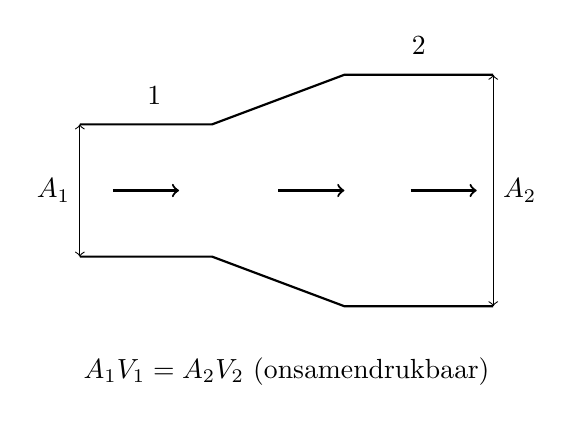
\begin{tikzpicture}[x=1.05cm,y=1.05cm]
        % nozzle
        \draw[thick] (0,0.8) -- (1.6,0.8) -- (3.2,1.4) -- (5.0,1.4);
        \draw[thick] (0,-0.8) -- (1.6,-0.8) -- (3.2,-1.4) -- (5.0,-1.4);

        % flow arrows
        \draw[->,thick] (0.4,0) -- (1.2,0);
        \draw[->,thick] (2.4,0) -- (3.2,0);
        \draw[->,thick] (4.0,0) -- (4.8,0);

        % areas
        \draw[<->] (0,-0.8) -- (0,0.8);
        \node[left] at (0,0) {$A_1$};
        \draw[<->] (5.0,-1.4) -- (5.0,1.4);
        \node[right] at (5.0,0) {$A_2$};

        % labels
        \node at (0.9,1.15) {1};
        \node at (4.1,1.75) {2};
        \node[below] at (2.5,-1.9) {$A_1V_1=A_2V_2$ (onsamendrukbaar)};
    \end{tikzpicture}
    \caption{Zelfde idee als Fig.~\ref{fig:continuity}: een vernauwing geeft hogere snelheid bij kleinere doorsnede.}
\end{figure}

\subsection{Impulsbehoud (Momentumvergelijking)}
Voor een controle volume geldt de impulsvergelijking:
\[
\sum \vec{F}_{ext} = \frac{\partial}{\partial t} \int_{CV} \rho \vec{v} \, dV + \int_{CS} \rho \vec{v} (\vec{v} \cdot \hat{n}) \, dA
\]
Voor stationaire stroming:
\[
\sum \vec{F}_{ext} = \int_{CS} \rho \vec{v} (\vec{v} \cdot \hat{n}) \, dA = \dot{m}_{uit} \vec{v}_{uit} - \dot{m}_{in} \vec{v}_{in}
\]
De externe krachten omvatten druk-, zwaarte- en wrijvingskrachten.

\begin{figure}[H]
    \centering
    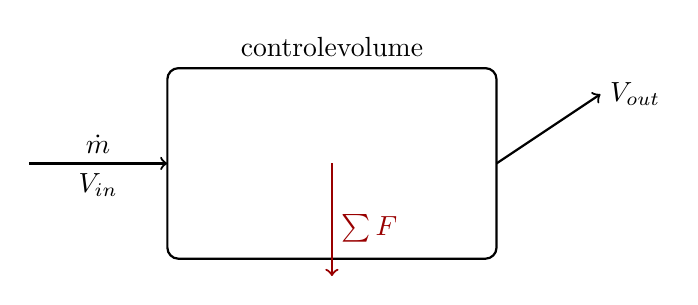
\begin{tikzpicture}[x=1.1cm,y=1.1cm]
        % control volume
        \draw[thick,rounded corners=4pt] (1.4,0.4) rectangle (5.2,2.6);
        \node at (3.3,2.85) {controlevolume};

        % jet in
        \draw[thick,->] (-0.2,1.5) -- (1.4,1.5);
        \node[above] at (0.6,1.5) {$\dot{m}$};
        \node[below] at (0.6,1.5) {$V_{in}$};

        % jet out (deflected)
        \draw[thick,->] (5.2,1.5) -- (6.4,2.3);
        \node[right] at (6.4,2.3) {$V_{out}$};

        % force
        \draw[thick,->,darkred] (3.3,1.5) -- (3.3,0.2);
        \node[darkred,right] at (3.3,0.75) {$\sum F$};
    \end{tikzpicture}
    \caption{Impulsbehoud: krachtresultante hangt samen met de verandering van impulsstroom door het controlevolume.}
\end{figure}

\subsubsection*{Voorbeeldoefening: straal op een plaat (orde van grootte)}
                	\textbf{Gegeven:} Waterstraal met massadebiet $\dot{m}=4{,}0\,\mathrm{kg/s}$ wordt idealiter omgebogen van $V_{in}=12\,\mathrm{m/s}$ naar stilstand in de $x$-richting (dus $V_{out,x}\approx 0$).\\
                	\textbf{Gevraagd:} Benader de kracht in $x$-richting op de plaat.\\
                	\textbf{Oplossing:}
Voor stationair: $\sum F_x\approx \dot{m}(V_{out,x}-V_{in,x})\approx 4.0\,(0-12)=-48\,\mathrm{N}$.\\
Dus de plaat ondervindt een kracht van \boxed{48\,\mathrm{N}} in de stromingsrichting (tegengesteld aan de snelheidsverandering).

\section{Afleiding van de Wet van Bernoulli}
\subsection{Afleiding via Euler Vergelijking}
De Euler vergelijking beschrijft de beweging van een ideaal (wrijvingsloos) fluïdum. Voor een stationaire stroming ($\frac{\partial \vec{v}}{\partial t} = 0$) luidt deze:
\[
\rho (\vec{v} \cdot \nabla)\vec{v} = -\nabla p + \rho \vec{g}
\]
Hierin is de term $(\vec{v} \cdot \nabla)\vec{v}$ de convectieve versnelling.

\subsection{Projectie op een Stroomlijn}
We vermenigvuldigen elke term van de Euler vergelijking scalair met een infinitesimale verplaatsing $d\vec{s}$ langs een stroomlijn. Omdat de snelheid $\vec{v}$ raakt aan de stroomlijn, is $d\vec{s}$ evenwijdig aan $\vec{v}$.
\[
\underbrace{\rho [(\vec{v} \cdot \nabla)\vec{v}] \cdot d\vec{s}}_{\text{Traagheidsterm}} = \underbrace{-\nabla p \cdot d\vec{s}}_{\text{Drukterm}} + \underbrace{\rho \vec{g} \cdot d\vec{s}}_{\text{Zwaartekrachtterm}}
\]
We werken elke term afzonderlijk uit:

\begin{itemize}
    \item \textbf{Drukterm:} De gradiënt $\nabla p$ is een vector die de richting van de grootste drukverandering aangeeft. Het inproduct met de verplaatsing $d\vec{s}$ geeft de totale verandering van de druk $dp$ over die afstand (totale differentiaal):
    \[ -\nabla p \cdot d\vec{s} = -\left( \frac{\partial p}{\partial x} dx + \frac{\partial p}{\partial y} dy + \frac{\partial p}{\partial z} dz \right) = -dp \]

    \item \textbf{Zwaartekrachtterm:} De zwaartekracht werkt verticaal omlaag: $\vec{g} = -g \hat{k} = (0, 0, -g)$. De verplaatsing is $d\vec{s} = (dx, dy, dz)$. Het inproduct wordt:
    \[ \rho \vec{g} \cdot d\vec{s} = \rho (0 \cdot dx + 0 \cdot dy - g \cdot dz) = -\rho g dz \]
    Dit komt overeen met de verandering in potentiële energie.

    \item \textbf{Traagheidsterm (Convectieve versnelling):} We gebruiken de vectoridentiteit $(\vec{v} \cdot \nabla)\vec{v} = \frac{1}{2}\nabla v^2 - \vec{v} \times (\nabla \times \vec{v})$.
    Het inproduct met $d\vec{s}$ wordt:
    \[ \rho \left( \frac{1}{2}\nabla v^2 - \vec{v} \times (\nabla \times \vec{v}) \right) \cdot d\vec{s} \]
    Omdat we integreren \textit{langs een stroomlijn}, is $d\vec{s}$ evenwijdig aan $\vec{v}$. Het vectorproduct $\vec{v} \times (\dots)$ staat loodrecht op $\vec{v}$ en dus ook loodrecht op $d\vec{s}$. Het inproduct van loodrechte vectoren is nul, dus de rotatieterm valt weg.
    \[ \rho \frac{1}{2}\nabla v^2 \cdot d\vec{s} = \rho d\left(\frac{1}{2}v^2\right) = \rho v dv \]
\end{itemize}

Invullen van deze termen in de oorspronkelijke vergelijking geeft:
\[
\rho v dv = -dp - \rho g dz
\]
Herschikken levert de differentiaalvergelijking van Bernoulli:
\[
dp + \rho v dv + \rho g dz = 0
\]
Voor een onsamendrukbare vloeistof ($\rho$ is constant) kunnen we integreren tussen twee punten op de stroomlijn:
\[
\int dp + \int \rho v dv + \int \rho g dz = \text{constant}
\]
Dit levert de wet van Bernoulli:
\[
p + \frac{1}{2}\rho v^2 + \rho g z = \text{constant}
\]

\subsection{Interpretatie van de Termen}
De wet van Bernoulli drukt behoud van mechanische energie uit per volume-eenheid:
\begin{itemize}
    \item $p$: Statische druk (drukenergie per volume)
    \item $\frac{1}{2}\rho v^2$: Dynamische druk (kinetische energie per volume)
    \item $\rho g z$: Hydrostatische druk (potentiële energie per volume)
\end{itemize}

\subsubsection*{Voorbeeld: Wet van Torricelli}
\textbf{Gegeven:} Een groot open reservoir gevuld met water heeft een klein gaatje op $5 \, m$ onder het wateroppervlak.
\textbf{Gevraagd:} De uitstroomsnelheid $V_2$.
\textbf{Oplossing:}
Pas Bernoulli toe tussen het oppervlak (1) en het gaatje (2).
$P_1 = P_2 = P_{atm}$ (beide open aan atmosfeer).
$V_1 \approx 0$ (reservoir is groot).
$z_1 = 5 \, m$, $z_2 = 0 \, m$.
\[
P_{atm} + 0 + \rho g (5) = P_{atm} + \frac{1}{2} \rho V_2^2 + 0
\]
\[
\rho g (5) = \frac{1}{2} \rho V_2^2 \implies V_2 = \sqrt{2 \cdot g \cdot 5}
\]
\[
V_2 = \sqrt{2 \cdot 9.81 \cdot 5} = \sqrt{98.1} \approx 9.9 \, m/s
\]

\begin{figure}[H]
    \centering
    \includegraphics[width=0.8\textwidth]{assets/bernoulli.png}
    \caption{Diagram van de Wet van Bernoulli.}
    \label{fig:bernoulli}
\end{figure}

\begin{figure}[H]
    \centering
    \includegraphics[width=0.82\textwidth]{assets/wikipedia/venturi_pd.png}
    \caption{Venturi-effect: hogere snelheid in de keel gaat (bij gelijke hoogte) samen met lagere statische druk.\;\scriptsize Bron: HappyApple, publiek domein, via Wikimedia Commons (\url{https://commons.wikimedia.org/wiki/File:Venturifixed2.PNG}).}
\end{figure}

\subsubsection*{Voorbeeldoefening: drukdaling in een venturi (Bernoulli + continuïteit)}
                	\textbf{Gegeven:} Water stroomt horizontaal door een venturi. Doorsneden: $A_2=0{,}50A_1$. Gemeten inlaat-snelheid $V_1=2{,}0\,\mathrm{m/s}$.\\
                	\textbf{Gevraagd:} Benader $p_1-p_2$ (verliesloos).\\
                	\textbf{Oplossing:}
Continuïteit: $A_1V_1=A_2V_2\Rightarrow V_2=\frac{A_1}{A_2}V_1=2V_1=4{,}0\,\mathrm{m/s}$.\\
Bernoulli (zelfde $z$): $p_1+\tfrac{1}{2}\rho V_1^2=p_2+\tfrac{1}{2}\rho V_2^2$.
\[
p_1-p_2=\frac{1}{2}\rho\left(V_2^2-V_1^2\right)=\frac{1}{2}\cdot 1000\,(16-4)=6000\,\mathrm{Pa}
\]
Dus \boxed{p_1-p_2\approx 6{,}0\,\mathrm{kPa}}.

\section{De Algemene Energievergelijking}
In de praktijk is er altijd wrijving en worden pompen of turbines gebruikt. We gebruiken dan de uitgebreide energievergelijking, vaak uitgedrukt in termen van "hoogte" (head, in meters vloeistofkolom):
\[
\frac{P_1}{\rho g} + \frac{V_1^2}{2g} + z_1 + h_{pomp} = \frac{P_2}{\rho g} + \frac{V_2^2}{2g} + z_2 + h_{turbine} + h_{L}
\]
Hierbij vertegenwoordigt $h_L$ het totaal aan energieverliezen (head loss) door wrijving in leidingen en componenten.

\chapter{Differentiële Analyse van Fluïdumstroming}
\section{Afleiding van de Navier-Stokes Vergelijkingen}
De Navier-Stokes vergelijkingen zijn de fundamentele bewegingsvergelijkingen voor viskeuze vloeistoffen. Ze zijn een uitbreiding van de Euler vergelijking (die wrijving verwaarloost) door toevoeging van viskeuze krachten.

\subsection{Newton's Tweede Wet voor een Fluïdumdeeltje}
We vertrekken opnieuw van de tweede wet van Newton ($\vec{F} = m\vec{a}$) toegepast op een infinitesimaal fluïdumdeeltje met volume $dV$ en massa $dm = \rho dV$.
\[
\rho dV \frac{D\vec{v}}{Dt} = \sum \vec{F}_{ext}
\]
Hierin is $\frac{D\vec{v}}{Dt}$ de materiële afgeleide (totale versnelling), die bestaat uit de lokale versnelling en de convectieve versnelling:
\[
\frac{D\vec{v}}{Dt} = \underbrace{\frac{\partial \vec{v}}{\partial t}}_{\text{lokaal}} + \underbrace{(\vec{v} \cdot \nabla)\vec{v}}_{\text{convectief}}
\]

\subsection{Krachtenbalans}
De krachten die op het deeltje werken kunnen worden onderverdeeld in lichaamskrachten en oppervlaktekrachten:
\[
\sum \vec{F}_{ext} = \vec{F}_{zwaartekracht} + \vec{F}_{druk} + \vec{F}_{viskeus}
\]

\begin{itemize}
    \item \textbf{Zwaartekracht:} Werkt op de massa van het deeltje.
    \[ \vec{F}_{zwaartekracht} = \rho \vec{g} \, dV \]

    \item \textbf{Drukkrachten:} Netto kracht door drukverschillen op de oppervlakken (normaalspanningen). Zoals eerder afgeleid bij Euler:
    \[ \vec{F}_{druk} = -\nabla p \, dV \]

    \item \textbf{Viskeuze krachten (Stroperigheid):} In een reëel fluïdum ontstaan er schuifspanningen door snelheidsgradiënten. Voor een \textit{Newtoniaans fluïdum} is de schuifspanning evenredig met de vervormingssnelheid. De evenredigheidsconstante is de dynamische viscositeit $\mu$.
    
    De netto viskeuze kracht per volume-eenheid is de divergentie van de viskeuze spanningstensor. Voor een onsamendrukbare stroming ($\nabla \cdot \vec{v} = 0$) vereenvoudigt dit tot:
    \[ \vec{F}_{viskeus} = \mu \nabla^2 \vec{v} \, dV \]
    Hierin is $\nabla^2 = \frac{\partial^2}{\partial x^2} + \frac{\partial^2}{\partial y^2} + \frac{\partial^2}{\partial z^2}$ de Laplace-operator. Deze term representeert de diffusie van impuls door wrijving.
\end{itemize}

\subsection{De Navier-Stokes Vergelijking}
Door alle termen in te vullen en te delen door het volume $dV$, verkrijgen we de Navier-Stokes vergelijking voor een onsamendrukbaar, Newtoniaans fluïdum:

\[
\underbrace{\rho \left( \frac{\partial \vec{v}}{\partial t} + (\vec{v} \cdot \nabla)\vec{v} \right)}_{\text{Traagheidskrachten}} = \underbrace{-\nabla p}_{\text{Drukkrachten}} + \underbrace{\mu \nabla^2 \vec{v}}_{\text{Viskeuze krachten}} + \underbrace{\rho \vec{g}}_{\text{Zwaartekracht}}
\]

Dit is een vectorvergelijking. In componentvorm (bijvoorbeeld de x-richting) ziet dit er als volgt uit:
\[
\rho \left( \frac{\partial u}{\partial t} + u \frac{\partial u}{\partial x} + v \frac{\partial u}{\partial y} + w \frac{\partial u}{\partial z} \right) = -\frac{\partial p}{\partial x} + \mu \left( \frac{\partial^2 u}{\partial x^2} + \frac{\partial^2 u}{\partial y^2} + \frac{\partial^2 u}{\partial z^2} \right) + \rho g_x
\]
Vergelijkbare vergelijkingen gelden voor de y- en z-richtingen. Samen met de continuïteitsvergelijking ($\nabla \cdot \vec{v} = 0$) vormen deze een gesloten stelsel om het stromingsveld te beschrijven.

\begin{figure}[H]
    \centering
    \includegraphics[width=0.6\textwidth]{assets/control_volume.png}
    \caption{Controlevolume voor de afleiding van behoudswetten.}
    \label{fig:control_volume}
\end{figure}

\section{Oplossing: Stroming tussen Parallelle Platen (Poiseuille)}
\textbf{Probleemstelling:} Stationaire, volledig ontwikkelde stroming tussen twee parallelle platen op afstand $a$ van elkaar.

\begin{figure}[H]
    \centering
    \includegraphics[width=0.8\textwidth]{assets/poiseuille_plates.png}
    \caption{Snelheidsprofiel voor laminaire stroming tussen parallelle platen.}
    \label{fig:poiseuille_plates}
\end{figure}

\textbf{Aannames:}
\begin{itemize}
    \item Stationair: $\frac{\partial}{\partial t} = 0$
    \item 2D stroming: $w = 0$
    \item Geen verandering in x-richting: $\frac{\partial u}{\partial x} = 0$
    \item Snelheid alleen in x-richting: $v = 0$
\end{itemize}

\textbf{Continuïteitsvergelijking:}
\[
\frac{\partial u}{\partial x} = 0 \Rightarrow u = u(y)
\]

\textbf{Navier-Stokes in x-richting:}
\[
0 = -\frac{\partial p}{\partial x} + \mu \frac{\partial^2 u}{\partial y^2}
\]

\textbf{Navier-Stokes in y-richting:}
\[
0 = -\frac{\partial p}{\partial y} \Rightarrow p = p(x)
\]

Omdat $\frac{\partial p}{\partial x}$ niet afhangt van $y$, en $\frac{\partial^2 u}{\partial y^2}$ niet afhangt van $x$, moet:
\[
\frac{\partial p}{\partial x} = \text{constant}
\]

\textbf{Integratie:}
\[
\frac{d^2 u}{dy^2} = \frac{1}{\mu} \frac{\partial p}{\partial x}
\]
Eerste integratie:
\[
\frac{du}{dy} = \frac{1}{\mu} \frac{\partial p}{\partial x} y + C_1
\]
Tweede integratie:
\[
u(y) = \frac{1}{2\mu} \frac{\partial p}{\partial x} y^2 + C_1 y + C_2
\]

\textbf{Randvoorwaarden:}
\begin{itemize}
    \item Bij $y=0$: $u(0) = 0$ (no-slip conditie)
    \item Bij $y=a$: $u(a) = U_p$ (snelheid van bovenste plaat)
\end{itemize}

\textbf{Toepassing van randvoorwaarden:}
\[
C_2 = 0
\]
\[
C_1 = \frac{U_p}{a} - \frac{1}{2\mu} \frac{\partial p}{\partial x} a
\]

\textbf{Oplossing:}
\[
u(y) = \frac{1}{2\mu} \frac{\partial p}{\partial x} y^2 + \left( \frac{U_p}{a} - \frac{1}{2\mu} \frac{\partial p}{\partial x} a \right) y
\]
Voor vaste platen ($U_p = 0$) wordt dit:
\[
u(y) = \frac{1}{2\mu} \frac{\partial p}{\partial x} (y^2 - ay)
\]

\section{Wet van Poiseuille voor Cilindrische Buis}
Voor stroming in een cilinder met straal $R$ geldt in cilindercoördinaten:
\[
u(r) = \frac{1}{4\mu} \frac{\partial p}{\partial x} (R^2 - r^2)
\]
Het volumedebiet is:
\[
Q = \int_0^R u(r) \, 2\pi r \, dr = -\frac{\pi}{8\mu} \frac{\partial p}{\partial x} R^4
\]
Met $\frac{\partial p}{\partial x} = \frac{p_2 - p_1}{L} = -\frac{\Delta p}{L}$:
\[
Q = \frac{\pi R^4 \Delta p}{8\mu L}
\]
Dit is de wet van Hagen-Poiseuille.

\subsubsection*{Voorbeeld: Drukval in een leiding}
\textbf{Gegeven:} Olie ($\mu = 0.2 \, Pa \cdot s$) stroomt door een horizontale buis met diameter $D = 2 \, cm$ en lengte $L = 10 \, m$. Het debiet is $Q = 0.5 \, liter/s = 0.0005 \, m^3/s$.
\textbf{Gevraagd:} Het drukverschil $\Delta p$.
\textbf{Oplossing:}
Straal $R = 0.01 \, m$.
\[
\Delta p = \frac{8 \mu L Q}{\pi R^4}
\]
\[
\Delta p = \frac{8 \cdot 0.2 \cdot 10 \cdot 0.0005}{\pi \cdot (0.01)^4}
\]
\[
\Delta p = \frac{0.008}{\pi \cdot 10^{-8}} \approx 254648 \, Pa \approx 2.55 \, bar
\]

\begin{figure}[H]
    \centering
    \includegraphics[width=0.7\textwidth]{assets/hagen_poiseuille.png}
    \caption{Parabolisch snelheidsprofiel bij Hagen-Poiseuille stroming in een buis.}
    \label{fig:hagen_poiseuille}
\end{figure}

\chapter{Interne en Externe Stroming}
\section{Interne Stroming: Laminair vs. Turbulent}
\subsection{Reynolds Getal}
Het Reynolds getal is een dimensieloze parameter die de verhouding tussen traagheids of inertiekrachten en viskeuze krachten aangeeft (intertiekracht/viscositeitskrachten):
\[
Re = \frac{\rho V D}{\mu} = \frac{V D}{\nu}
\]
waarbij:
\begin{itemize}
    \item $V$: karakteristieke snelheid [m/s]
    \item $D$: karakteristieke lengte (bijv. diameter) [m]
    \item $\rho$: dichtheid [kg/m³]
    \item $\mu$: dynamische viscositeit [Pa·s]
    \item $\nu$: kinematische viscositeit [m²/s]
\end{itemize}

\symS{Re}{Reynoldsgetal}{-}
\symS{D}{karakteristieke lengte (bijv. diameter)}{m}

\subsection{Overgang Laminair-Turbulent}
Voor stroming in een cilinderbuis:
\begin{itemize}
    \item \textbf{Laminair ($Re < 2000$):} De vloeistof stroomt in ordelijke, parallelle lagen. Viscositeit domineert en verstoringen worden uitgedempt. Het snelheidsprofiel is parabolisch ($V_{max} = 2 V_{gem}$).
    \item \textbf{Transitiegebied ($2000 < Re < 3000$):} De stroming wisselt tussen laminair en turbulent.
    \item \textbf{Turbulent ($Re > 3000$):} De stroming is chaotisch met wervelingen en sterke menging. Traagheidskrachten domineren. Het snelheidsprofiel is veel vlakker ("plug flow").
\end{itemize}

\begin{figure}[H]
    \centering
    \includegraphics[width=0.6\textwidth]{assets/laminar_turbulent.png}
    \caption{Visuele weergave van laminaire (boven) en turbulente (onder) stroming, zoals zichtbaar gemaakt met kleurstofinjectie (Osborne Reynolds experiment).}
    \label{fig:laminar_turbulent}
\end{figure}

\begin{figure}[H]
    \centering
    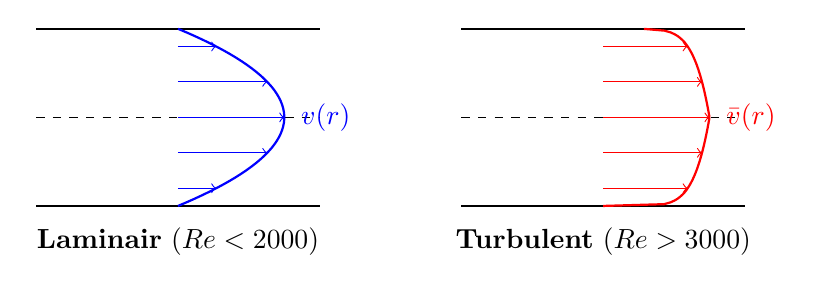
\begin{tikzpicture}[scale=0.9]
        % Laminar
        \begin{scope}[xshift=0cm]
            \draw[thick] (0,2.5) -- (4,2.5);
            \draw[thick] (0,0) -- (4,0);
            \draw[dashed] (0,1.25) -- (4,1.25);
            \node at (2, -0.5) {\textbf{Laminair} ($Re < 2000$)};
            
            % Parabolic profile: v = vmax * (1 - (r/R)^2)
            % y goes from 0 to 2.5. Center at 1.25. R = 1.25.
            % r = y - 1.25.
            \draw[thick, blue, domain=0:2.5, samples=50] plot ({2 + 1.5*(1 - (((\x-1.25)/1.25)^2))}, \x);
            
            % Arrows
            \foreach \y in {0.25, 0.75, 1.25, 1.75, 2.25} {
                \draw[->, blue] (2, \y) -- ({2 + 1.5*(1 - (((\y-1.25)/1.25)^2))}, \y);
            }
            \node[blue, right] at (3.6, 1.25) {$v(r)$};
        \end{scope}
        
        % Turbulent
        \begin{scope}[xshift=6cm]
            \draw[thick] (0,2.5) -- (4,2.5);
            \draw[thick] (0,0) -- (4,0);
            \draw[dashed] (0,1.25) -- (4,1.25);
            \node at (2, -0.5) {\textbf{Turbulent} ($Re > 3000$)};
            
            % Power law profile: v = vmax * (1 - r/R)^(1/7)
            \draw[thick, red, domain=0:2.5, samples=100] plot ({2 + 1.5*((1 - abs((\x-1.25)/1.25))^(1/7))}, \x);
            
            % Arrows
            \foreach \y in {0.25, 0.75, 1.25, 1.75, 2.25} {
                \draw[->, red] (2, \y) -- ({2 + 1.5*((1 - abs((\y-1.25)/1.25))^(1/7))}, \y);
            }
             \node[red, right] at (3.6, 1.25) {$\bar{v}(r)$};
        \end{scope}
    \end{tikzpicture}
    \caption{Vergelijking van snelheidsprofielen: Laminair (parabolisch) vs. Turbulent (vlakker profiel).}
    \label{fig:velocity_profiles_comparison}
\end{figure}

\subsubsection*{Voorbeeld: Reynoldsgetal bepalen}
\textbf{Gegeven:} Water ($20^\circ C$, $\nu = 10^{-6} \, m^2/s$) stroomt door een buis met diameter $50 \, mm$ met een gemiddelde snelheid van $0.1 \, m/s$.
\textbf{Gevraagd:} Is de stroming laminair of turbulent?
\textbf{Oplossing:}
\[
Re = \frac{V D}{\nu} = \frac{0.1 \cdot 0.05}{10^{-6}} = \frac{0.005}{10^{-6}} = 5000
\]
Omdat $Re = 5000 > 3000$, is de stroming \textbf{turbulent}.

\subsection{Reynolds Decompositie}
In turbulente stroming wordt de momentane snelheid ontbonden in een tijdsgemiddelde en een fluctuerende component:
\[
u(t,y) = \bar{u}(y) + u'(t,y)
\]
waarbij $\bar{u}(y)$ de tijdsgemiddelde snelheid is en $u'(t,y)$ de turbulente fluctuatie (met $\overline{u'} = 0$).
De turbulente fluctuaties veroorzaken een extra schijnbare schuifspanning, de Reynoldsspanning: $\tau_{Reynolds} = -\rho \overline{u'v'}$. Deze verhoogt de effectieve wrijving in turbulente stroming aanzienlijk.

\subsection{Wrijvingsfactor en Drukval}
Het energieverlies door wrijving in een rechte leiding resulteert in een drukval $\Delta p$. Deze wordt berekend met de \textbf{Darcy-Weisbach vergelijking}:
\[
\Delta p = f \frac{L}{D} \frac{1}{2}\rho V^2
\]
Of uitgedrukt als wrijvingshoogte (head loss):
\[
h_f = \frac{\Delta p}{\rho g} = f \frac{L}{D} \frac{V^2}{2g}
\]
Hierin is:
\begin{itemize}
    \item $f$: de Darcy-wrijvingsfactor (dimensieloos)
    \item $L$: lengte van de leiding [m]
    \item $D$: diameter van de leiding [m]
    \item $V$: gemiddelde stroomsnelheid [m/s]
\end{itemize}

\subsubsection{Bepaling van de Wrijvingsfactor $f$}
De waarde van $f$ hangt af van het stromingsregime (Reynoldsgetal) en de wandruwheid.

\textbf{1. Laminaire stroming ($Re < 2000$):}
Bij laminaire stroming wordt de wrijving puur bepaald door viskeuze krachten en is de wandruwheid verwaarloosbaar. De factor $f$ volgt uit een exacte analytische oplossing (Hagen-Poiseuille):
\[
f = \frac{64}{Re}
\]

\textbf{2. Turbulente stroming ($Re > 3000$):}
Bij turbulente stroming spelen zowel de viskeuze sublaag als de wandruwheid een rol. De wrijvingsfactor hangt af van:
\begin{itemize}
    \item Het Reynoldsgetal $Re$
    \item De relatieve wandruwheid $\varepsilon/D$ (waarbij $\varepsilon$ de gemiddelde ruwheidshoogte is)
\end{itemize}

De waarde van $f$ kan worden afgelezen uit het \textbf{Moody-diagram} (Figuur \ref{fig:moody}) of berekend met de impliciete \textbf{Colebrook-vergelijking}:
\[
\frac{1}{\sqrt{f}} = -2 \log_{10} \left( \frac{\varepsilon/D}{3.7} + \frac{2.51}{Re \sqrt{f}} \right)
\]
Voor handberekeningen is de \textbf{Haaland-benadering} (expliciet) vaak nauwkeurig genoeg:
\[
\frac{1}{\sqrt{f}} \approx -1.8 \log_{10} \left( \left( \frac{\varepsilon/D}{3.7} \right)^{1.11} + \frac{6.9}{Re} \right)
\]

\begin{figure}[H]
    \centering
    \includegraphics[width=0.8\textwidth]{assets/moody_diagram.png}
    \caption{Moody-diagram: $f$ als functie van $Re$ en relatieve ruwheid $\varepsilon/D$.}
    \label{fig:moody}
\end{figure}

\subsubsection*{Voorbeeldoefening: Drukverlies in een waterleiding}
\textbf{Gegeven:} Water ($\rho=1000\,\mathrm{kg/m^3}$, $\nu=10^{-6}\,\mathrm{m^2/s}$) stroomt door een horizontale stalen buis ($\varepsilon=0.045\,\mathrm{mm}$) met een diameter $D=50\,\mathrm{mm}$ en lengte $L=20\,\mathrm{m}$. De snelheid is $V=4.0\,\mathrm{m/s}$.\\
\textbf{Gevraagd:} Bereken de drukval $\Delta p$ over de leiding.\\
\textbf{Oplossing:}
\begin{enumerate}
    \item \textbf{Bereken Reynoldsgetal:}
    \[ Re = \frac{VD}{\nu} = \frac{4.0 \cdot 0.050}{10^{-6}} = 200\,000 \]
    Dit is $>3000$, dus de stroming is \textbf{turbulent}.
    
    \item \textbf{Bepaal relatieve ruwheid:}
    \[ \frac{\varepsilon}{D} = \frac{0.045\,\mathrm{mm}}{50\,\mathrm{mm}} = 0.0009 \]
    
    \item \textbf{Bepaal wrijvingsfactor $f$:}
    Via Moody-diagram bij $Re=2\cdot 10^5$ en $\varepsilon/D=0.0009$ vinden we $f \approx 0.021$.
    (Of via Haaland formule: $f \approx 0.0208$).
    
    \item \textbf{Bereken drukval:}
    \[ \Delta p = f \frac{L}{D} \frac{1}{2}\rho V^2 = 0.021 \cdot \frac{20}{0.050} \cdot \frac{1}{2} \cdot 1000 \cdot (4.0)^2 \]
    \[ \Delta p = 0.021 \cdot 400 \cdot 8000 = 67\,200\,\mathrm{Pa} \]
\end{enumerate}
De drukval is dus \boxed{67.2\,\mathrm{kPa}}.

\subsection{Major en Minor Losses}
In leidingsystemen wordt het totale energieverlies (head loss, $h_L$) onderverdeeld in twee categorieën:

\subsubsection{Major Losses (Wrijvingsverliezen)}
Dit zijn de verliezen door viskeuze wrijving in de rechte stukken leiding. Zoals eerder besproken worden deze berekend met Darcy-Weisbach:
\[ h_{major} = f \frac{L}{D} \frac{V^2}{2g} \]
Hoewel ze "major" heten, zijn ze niet altijd de grootste verliezen; de naam verwijst naar het feit dat ze over de hele lengte optreden.

\subsubsection{Minor Losses (Lokale Verliezen)}
Dit zijn verliezen die optreden bij componenten zoals bochten, afsluiters, vernauwingen, verwijdingen en in- of uitlaten. Deze verliezen worden veroorzaakt door stroomloslating en wervelingen die energie dissiperen.
\[ h_{minor} = K_L \frac{V^2}{2g} \]
Hierin is $K_L$ de verliescoëfficiënt (loss coefficient), die afhangt van de geometrie van de component.
Enkele typische waarden voor $K_L$:
\begin{itemize}
    \item Scherpe inlaat: $K_L \approx 0.5$
    \item Afgeronde inlaat: $K_L \approx 0.04$
    \item Uitlaat (in reservoir): $K_L = 1.0$ (alle kinetische energie gaat verloren)
    \item 90$^\circ$ bocht (standaard): $K_L \approx 0.3 - 0.9$
    \item Volledig open bolkraan: $K_L \approx 10$
\end{itemize}

Soms wordt ook de equivalente lengte $L_{eq}$ gebruikt: $h_{minor} = f \frac{L_{eq}}{D} \frac{V^2}{2g}$.

\begin{figure}[H]
    \centering
    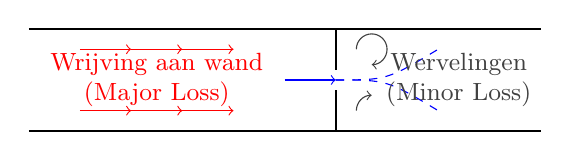
\begin{tikzpicture}[scale=1.3]
        % Pipe
        \draw[thick] (0,1) -- (5,1);
        \draw[thick] (0,0) -- (5,0);
        
        % Major Loss
        \foreach \x in {0.5, 1.0, 1.5} {
            \draw[->, red] (\x, 0.8) -- (\x+0.5, 0.8);
            \draw[->, red] (\x, 0.2) -- (\x+0.5, 0.2);
        }
        \node[red, align=center, font=\small] at (1.25, 0.5) {Wrijving aan wand\\(Major Loss)};
        
        % Minor Loss (Orifice plate)
        \draw[thick, fill=gray] (3, 1) -- (3, 0.6);
        \draw[thick, fill=gray] (3, 0) -- (3, 0.4);
        
        % Streamlines
        \draw[blue, ->] (2.5, 0.5) -- (3, 0.5);
        \draw[blue, dashed] (3, 0.5) .. controls (3.5, 0.5) .. (4, 0.8);
        \draw[blue, dashed] (3, 0.5) .. controls (3.5, 0.5) .. (4, 0.2);
        
        % Eddies
        \draw[->, darkgray] (3.2, 0.8) arc (180:-90:0.15);
        \draw[->, darkgray] (3.2, 0.2) arc (180:90:0.15);
        \node[darkgray, align=center, font=\small] at (4.2, 0.5) {Wervelingen\\(Minor Loss)};
    \end{tikzpicture}
    \caption{Illustratie van Major Losses (wandwrijving) en Minor Losses (wervelingen door obstructies).}
    \label{fig:losses_concept}
\end{figure}

\subsubsection{Totale Head Loss}
Het totale verlies is de som van alle major en minor losses in het systeem:
\[ h_{L,totaal} = \sum h_{major} + \sum h_{minor} = \sum f_i \frac{L_i}{D_i} \frac{V_i^2}{2g} + \sum K_{L,j} \frac{V_j^2}{2g} \]
Als de diameter (en dus snelheid $V$) constant is over het hele systeem, kan dit vereenvoudigd worden tot:
\[ h_{L,totaal} = \left( f \frac{L}{D} + \sum K_L \right) \frac{V^2}{2g} \]

\subsubsection*{Voorbeeldoefening: Leidingsysteem met verliezen}
\textbf{Gegeven:} Water stroomt uit een groot reservoir door een horizontale pijp ($D=10\,\mathrm{cm}$, $L=50\,\mathrm{m}$, $f=0.02$) naar de atmosfeer. Het systeem bevat:
\begin{itemize}
    \item Een scherpe inlaat ($K_L=0.5$)
    \item Twee 90$^\circ$ bochten ($K_L=0.3$ elk)
    \item Een volledig open afsluiter ($K_L=0.2$)
\end{itemize}
Het waterniveau in het reservoir staat $H=10\,\mathrm{m}$ boven de uitlaat.

\begin{figure}[H]
    \centering
    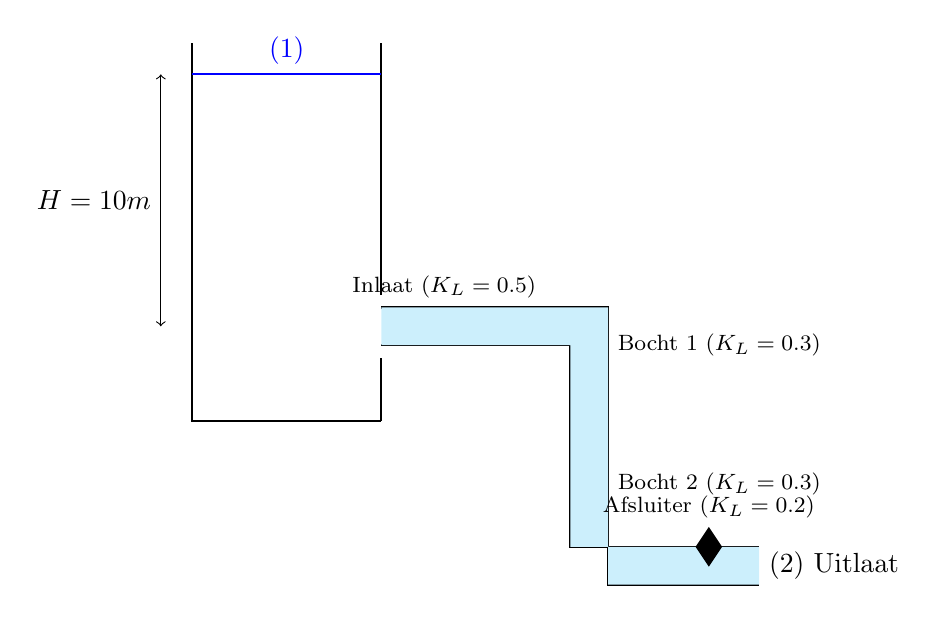
\begin{tikzpicture}[scale=0.8]
        % Tank
        \draw[thick] (0, 5) -- (0, 0) -- (3, 0);
        \draw[thick] (0, 5) -- (0, 6);
        \draw[thick] (3, 0) -- (3, 1);
        \draw[thick] (3, 2) -- (3, 6);
        
        % Water
        \draw[blue, thick] (0, 5.5) -- (3, 5.5);
        \node[blue, above] at (1.5, 5.5) {(1)};
        \draw[<->] (-0.5, 5.5) -- (-0.5, 1.5) node[midway, left] {$H=10m$};
        
        % Pipe segments (schematic)
        \draw[thick] (3, 1.2) -- (6, 1.2) -- (6, -2) -- (9, -2);
        \draw[thick] (3, 1.8) -- (6.6, 1.8) -- (6.6, -2.6) -- (9, -2.6);
        
        % Fill water
        \fill[cyan!20] (3, 1.2) -- (6, 1.2) -- (6, -2) -- (9, -2) -- (9, -2.6) -- (6.6, -2.6) -- (6.6, 1.8) -- (3, 1.8) -- cycle;
        
        % Components labels
        \node[above, font=\footnotesize] at (4, 1.8) {Inlaat ($K_L=0.5$)};
        \node[right, font=\footnotesize] at (6.6, 1.2) {Bocht 1 ($K_L=0.3$)};
        \node[right, font=\footnotesize] at (6.6, -1.0) {Bocht 2 ($K_L=0.3$)};
        
        % Valve
        \draw[fill=black] (8, -2) -- (8.2, -1.7) -- (8.4, -2) -- (8.2, -2.3) -- cycle;
        \node[above, font=\footnotesize] at (8.2, -1.7) {Afsluiter ($K_L=0.2$)};
        
        % Exit
        \node[right] at (9, -2.3) {(2) Uitlaat};
        
    \end{tikzpicture}
    \caption{Schematische voorstelling van het leidingsysteem uit de oefening.}
    \label{fig:exercise_losses}
\end{figure}

\textbf{Gevraagd:} Het debiet $Q$.\\
\textbf{Oplossing:}
We passen de uitgebreide Bernoulli-vergelijking toe tussen het oppervlak van het reservoir (1) en de uitlaat (2):
\[ \frac{p_1}{\rho g} + \frac{V_1^2}{2g} + z_1 = \frac{p_2}{\rho g} + \frac{V_2^2}{2g} + z_2 + h_L \]
\begin{itemize}
    \item $p_1 = p_2 = p_{atm}$ (beide open aan atmosfeer) $\rightarrow$ vallen weg.
    \item $V_1 \approx 0$ (groot reservoir).
    \item $z_1 - z_2 = H = 10\,\mathrm{m}$.
\end{itemize}
De vergelijking wordt:
\[ H = \frac{V_2^2}{2g} + h_L \]
Het totale verlies is:
\[ h_L = \left( f \frac{L}{D} + \sum K_L \right) \frac{V_2^2}{2g} \]
Waarbij $\sum K_L = K_{inlaat} + 2 \cdot K_{bocht} + K_{afsluiter} = 0.5 + 2(0.3) + 0.2 = 1.3$.
Invullen:
\[ 10 = \frac{V_2^2}{2g} + \left( 0.02 \frac{50}{0.10} + 1.3 \right) \frac{V_2^2}{2g} \]
\[ 10 = \frac{V_2^2}{2g} \left( 1 + 0.02 \cdot 500 + 1.3 \right) = \frac{V_2^2}{2g} (1 + 10 + 1.3) = \frac{V_2^2}{2g} (12.3) \]
\[ V_2^2 = \frac{10 \cdot 2 \cdot 9.81}{12.3} = \frac{196.2}{12.3} \approx 15.95 \]
\[ V_2 = \sqrt{15.95} \approx 3.99\,\mathrm{m/s} \]
Het debiet is $Q = V_2 \cdot A = 3.99 \cdot \frac{\pi}{4}(0.10)^2 = 3.99 \cdot 0.007854 \approx 0.0313\,\mathrm{m^3/s}$.
Dus \boxed{Q \approx 31.3\,\mathrm{L/s}}.

\section{Externe Stroming: Weerstand en Lift}
Bij externe stroming beweegt een fluïdum rondom een object (of beweegt een object door een stilstaand fluïdum). De krachten die het fluïdum op het object uitoefent, worden ontbonden in twee componenten:
\begin{itemize}
    \item \textbf{Weerstand (Drag, $F_D$):} De krachtcomponent evenwijdig aan de stromingsrichting (remmend).
    \item \textbf{Lift ($F_L$):} De krachtcomponent loodrecht op de stromingsrichting.
\end{itemize}

\subsection{Weerstand (Drag)}
De totale weerstandskracht wordt gegeven door:
\[
F_D = C_D A \frac{1}{2} \rho V^2
\]
Hierin is:
\begin{itemize}
    \item $C_D$: de weerstandscoëfficiënt (dimensieloos, experimenteel bepaald).
    \item $A$: het frontaal oppervlak (geprojecteerd oppervlak loodrecht op de stroming).
    \item $\rho$: de dichtheid van het fluïdum.
    \item $V$: de relatieve snelheid.
\end{itemize}

De weerstand bestaat uit twee bijdragen:
\begin{enumerate}
    \item \textbf{Wrijvingsweerstand:} Veroorzaakt door schuifspanningen aan het oppervlak (viscositeit). Dominant bij slanke, gestroomlijnde lichamen (zoals een vliegtuigvleugel).
    \item \textbf{Drukweerstand (Vormweerstand):} Veroorzaakt door drukverschillen. Aan de voorkant is de druk hoog (stuwpunt), aan de achterkant laag, vooral als de stroming loslaat (\textit{flow separation}) en een turbulent zog vormt. Dominant bij stompe voorwerpen (zoals een bal of vrachtwagen).
\end{enumerate}

\begin{figure}[H]
    \centering
    \includegraphics[width=0.5\textwidth]{assets/drag_coefficient.png}
    \caption{Weerstandscoëfficiënt van een bol als functie van het Reynoldsgetal. Merk de plotse daling op bij $Re \approx 3 \cdot 10^5$ (overgang naar turbulente grenslaag, waardoor loslating wordt uitgesteld).}
    \label{fig:drag_coeff}
\end{figure}

\subsubsection*{Voorbeeldoefening: Weerstand op een auto}
\textbf{Gegeven:} Een auto met frontaal oppervlak $A = 2.4 \, m^2$ en $C_D = 0.30$ rijdt met $108 \, km/u$ door lucht ($\rho = 1.2 \, kg/m^3$).\\
\textbf{Gevraagd:} Het vermogen nodig om de luchtweerstand te overwinnen.\\
\textbf{Oplossing:}
\begin{enumerate}
    \item Zet snelheid om naar m/s: $V = 108 / 3.6 = 30 \, m/s$.
    \item Bereken de weerstandskracht:
    \[ F_D = C_D A \frac{1}{2} \rho V^2 = 0.30 \cdot 2.4 \cdot \frac{1}{2} \cdot 1.2 \cdot (30)^2 = 0.30 \cdot 2.4 \cdot 0.6 \cdot 900 = 388.8 \, N \]
    \item Bereken het vermogen ($P = F \cdot V$):
    \[ P = F_D \cdot V = 388.8 \, N \cdot 30 \, m/s = 11664 \, W \approx 11.7 \, kW \]
\end{enumerate}
Het benodigde vermogen is \boxed{11.7 \, kW}.

\subsection{Lift}
Lift wordt gegenereerd door een asymmetrische stroming rond een lichaam, waardoor de druk aan de ene kant lager is dan aan de andere kant (Bernoulli: hogere snelheid = lagere druk).
\[
F_L = C_L A \frac{1}{2} \rho V^2
\]
Hier is $A$ meestal het \textit{planform area} (bovenaanzicht oppervlak) bij vleugels, niet het frontaal oppervlak.

\begin{figure}[H]
    \centering
    \includegraphics[width=0.4\textwidth]{assets/Lift.png}
    \caption{Krachtenbalans op een vleugelprofiel: Lift loodrecht op de stroming, Drag evenwijdig.}
\end{figure}

\subsubsection*{Voorbeeldoefening: Opstijgend vliegtuig}
\textbf{Gegeven:} Een vliegtuigje (massa $1500 \, kg$) moet opstijgen. Vleugeloppervlak $A = 20 \, m^2$. Maximale liftcoëfficiënt $C_{L,max} = 1.5$. Luchtdichtheid $\rho = 1.2 \, kg/m^3$.\\
\textbf{Gevraagd:} De minimale opstijgsnelheid (stall speed).\\
\textbf{Oplossing:}
Om op te stijgen moet de liftkracht gelijk zijn aan het gewicht ($F_L = m \cdot g$).
\[ m g = C_{L,max} A \frac{1}{2} \rho V_{min}^2 \]
Herschrijven voor $V_{min}$:
\[ V_{min} = \sqrt{\frac{2 m g}{C_{L,max} \rho A}} \]
Invullen:
\[ V_{min} = \sqrt{\frac{2 \cdot 1500 \cdot 9.81}{1.5 \cdot 1.2 \cdot 20}} = \sqrt{\frac{29430}{36}} = \sqrt{817.5} \approx 28.6 \, m/s \]
De minimale snelheid is \boxed{28.6 \, m/s} (ongeveer $103 \, km/u$).


\part{Warmte}

\chapter{Fundamentele Concepten van de Thermodynamica}
Thermodynamica is de wetenschap van energie, afgeleid van de Griekse woorden therme (warmte) en dynamis (kracht). Historisch gezien ontstond deze wetenschap uit de wens om warmte om te zetten in mechanische arbeid, met name tijdens de industriële revolutie. Tegenwoordig omvat het concept energie veel meer dan alleen warmte en arbeid; het is een centraal begrip in het begrijpen van chemische reacties, faseovergangen en zelfs het uitdijen van het heelal.

\section{Systemen en Controle Volumes}
Een fundamentele eerste stap in elke thermodynamische analyse is het definiëren van het object van studie: het systeem. Een systeem wordt gedefinieerd als een hoeveelheid materie of een gebied in de ruimte dat gekozen is voor analyse. Alles buiten het systeem wordt de omgeving genoemd. De scheiding tussen het systeem en de omgeving is de grens (boundary). Deze grens kan fysiek zijn (zoals de wand van een tank) of imaginair (zoals de open uitlaat van een pijp), en kan zowel vast als bewegend zijn.

We onderscheiden twee hoofdtypen systemen, die elk een eigen wiskundige benadering vereisen:
\begin{description}
    \item[Gesloten Systeem (Controlemassa):] Bij een gesloten systeem is de hoeveelheid massa vast. Er kan geen massa de grens van het systeem passeren. Energie, in de vorm van warmte of arbeid, kan de grens echter wel passeren. Een klassiek voorbeeld is een gas opgesloten in een zuiger-cilinder apparaat. Als het gas wordt verwarmd, zet het uit en beweegt de zuiger. De grens van het systeem beweegt dus en het volume verandert, maar de massa binnenin blijft constant. Als er ook geen energie de grens passeert, spreken we van een geïsoleerd systeem.
    \item[Open Systeem (Controlevolume):] In veel technische toepassingen, zoals bij compressoren, turbines, en straalmotoren, is er sprake van een continue stroom van massa. In deze gevallen is het handiger om een specifiek volume in de ruimte te bestuderen, het zogenaamde controlevolume. De grenzen van dit volume worden het controleoppervlak genoemd. Zowel massa als energie kunnen deze grenzen passeren. Een boiler is bijvoorbeeld een open systeem: koud water stroomt erin, warmte wordt toegevoegd, en warm water stroomt eruit.
\end{description}

\symW{Q}{warmteoverdracht (gesloten systeem)}{J}
\symW{W}{arbeid (gesloten systeem)}{J}
\symW{\dot{m}}{massadebiet}{kg/s}
\symW{h}{specifieke enthalpie}{kJ/kg}

\begin{figure}[H]
    \centering
    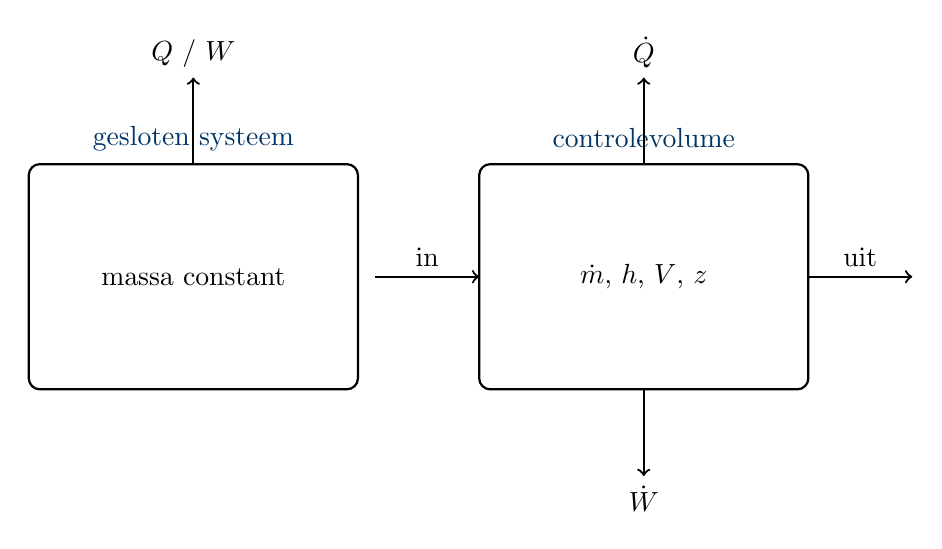
\begin{tikzpicture}[x=1.1cm,y=1.1cm]
        % closed system
        \draw[thick,rounded corners=4pt] (0,0) rectangle (3.8,2.6);
        \node[darkblue] at (1.9,2.9) {gesloten systeem};
        \node at (1.9,1.3) {massa constant};
        \draw[thick,->] (1.9,2.6) -- (1.9,3.6);
        \node[above] at (1.9,3.6) {$Q$ / $W$};

        % open system
        \draw[thick,rounded corners=4pt] (5.2,0) rectangle (9.0,2.6);
        \node[darkblue] at (7.1,2.9) {controlevolume};
        \draw[thick,->] (4.0,1.3) -- (5.2,1.3);
        \node[above] at (4.6,1.3) {in};
        \draw[thick,->] (9.0,1.3) -- (10.2,1.3);
        \node[above] at (9.6,1.3) {uit};
        \node at (7.1,1.3) {$\dot{m}$, $h$, $V$, $z$};
        \draw[thick,->] (7.1,2.6) -- (7.1,3.6);
        \node[above] at (7.1,3.6) {$\dot{Q}$};
        \draw[thick,->] (7.1,0) -- (7.1,-1.0);
        \node[below] at (7.1,-1.0) {$\dot{W}$};
    \end{tikzpicture}
    \caption{Thermodynamische modellering: gesloten systeem (controlemassa) vs. open systeem (controlevolume).}
\end{figure}

\section{Eigenschappen van een Systeem}
Elk systeem wordt gekarakteriseerd door zijn eigenschappen. Dit zijn macroscopische kenmerken zoals druk ($P$), temperatuur ($T$), volume ($V$) en massa ($m$). Thermodynamische eigenschappen kunnen worden onderverdeeld in twee categorieën:
\symW{P}{druk}{Pa}
\symW{T}{temperatuur}{K}
\symW{V}{volume}{m$^3$}
\symW{m}{massa}{kg}
\begin{itemize}
    \item \textbf{Intensieve eigenschappen:} Deze zijn onafhankelijk van de massa of de grootte van het systeem. Voorbeelden zijn temperatuur, druk en dichtheid. Als men een systeem in thermisch evenwicht in tweeën deelt, behouden beide helften dezelfde temperatuur en druk als het origineel.
    \item \textbf{Extensieve eigenschappen:} Deze waarden zijn afhankelijk van de grootte van het systeem. Voorbeelden zijn de totale massa, het totale volume en de totale energie. De waarde van een extensieve eigenschap voor het gehele systeem is de som van de waarden voor de onderdelen.
\end{itemize}
Om intensieve en extensieve eigenschappen te koppelen, gebruiken we vaak specifieke eigenschappen. Dit zijn extensieve eigenschappen per eenheid massa. Bijvoorbeeld:
\begin{itemize}
    \item Specifiek volume ($v$): $v = V/m$ (m³/kg)
    \item Specifieke interne energie ($u$): $u = U/m$ (kJ/kg)
    \item Specifieke enthalpie ($h$): $h = H/m$ (kJ/kg)
\end{itemize}
Specifieke eigenschappen zijn intensief, omdat ze niet afhangen van de totale hoeveelheid massa in het systeem.

\section{Toestand en Evenwicht}
De toestand van een systeem wordt volledig beschreven door zijn eigenschappen. Echter, we hoeven niet alle eigenschappen te meten om de toestand vast te leggen. Het State Postulate stelt dat de toestand van een eenvoudig samendrukbaar systeem volledig bepaald is door twee onafhankelijke intensieve eigenschappen.

Dit is een cruciaal concept. "Eenvoudig samendrukbaar" betekent dat effecten van elektrische, magnetische, zwaartekracht- en oppervlaktespanningsvelden verwaarloosbaar zijn. "Onafhankelijk" betekent dat de ene eigenschap kan variëren terwijl de andere constant blijft. Bijvoorbeeld, temperatuur en specifiek volume zijn altijd onafhankelijk en kunnen samen de toestand bepalen. Temperatuur en druk zijn echter niet onafhankelijk tijdens een faseovergang (zoals kokend water), omdat de kooktemperatuur vastligt bij een bepaalde druk.

Thermodynamica behandelt voornamelijk evenwichtstoestanden. Evenwicht impliceert een staat van balans waarin er geen drijvende krachten meer zijn die verandering veroorzaken:
\begin{itemize}
    \item \textbf{Thermisch evenwicht:} De temperatuur is overal in het systeem gelijk.
    \item \textbf{Mechanisch evenwicht:} De druk is in het systeem constant in de tijd (hoewel deze kan variëren met de hoogte door zwaartekracht).
    \item \textbf{Fase-evenwicht:} De massa van elke fase (bijv. vloeistof en damp) blijft constant.
    \item \textbf{Chemisch evenwicht:} De chemische samenstelling verandert niet in de tijd.
\end{itemize}

\section{Processen en Cycli}
Wanneer een systeem verandert van de ene evenwichtstoestand naar de andere, ondergaat het een proces. De reeks toestanden die het systeem doorloopt, vormt het pad van het proces. Om een proces volledig te beschrijven, moeten we de begintoestand, de eindtoestand, het pad en de interacties met de omgeving (warmte en arbeid) kennen.

Vaak wordt in analyses aangenomen dat een proces een quasi-evenwichtsproces (of quasi-statisch proces) is. Dit houdt in dat het proces zo langzaam verloopt dat het systeem op elk moment infinitesimaal dicht bij een evenwichtstoestand is. Hoewel dit een idealisatie is, benadert het veel werkelijke processen goed en maakt het berekeningen eenvoudiger omdat de eigenschappen uniform gedefinieerd blijven.

Speciale processen worden aangeduid met het voorvoegsel iso-:
\begin{itemize}
    \item \textbf{Isotherm:} Temperatuur blijft constant ($T = C$).
    \item \textbf{Isobaar:} Druk blijft constant ($P = C$).
    \item \textbf{Isochoor:} Volume blijft constant ($V = C$).
    \item \textbf{Adiabatisch:} Er is geen warmte-uitwisseling met de omgeving ($Q = 0$). Let op: adiabatisch betekent niet noodzakelijk dat de temperatuur constant is; expansie zonder warmtetoevoer leidt bijvoorbeeld tot afkoeling.
\end{itemize}
Een cyclus is een proces (of reeks processen) waarbij de eindtoestand identiek is aan de begintoestand. De netto verandering van eigenschappen over een cyclus is nul ($\Delta E_{cyclus} = 0$), wat impliceert dat de netto energieoverdracht via warmte gelijk moet zijn aan de netto energieoverdracht via arbeid.

\chapter{De Eerste Hoofdwet van de Thermodynamica: Energiebehoud}
De Eerste Hoofdwet van de thermodynamica is een uitdrukking van het principe van behoud van energie: energie kan niet worden gecreëerd of vernietigd, alleen van vorm veranderen. Voor elk thermodynamisch systeem geldt:
\[
E_{in} - E_{uit} = \Delta E_{systeem}
\]
De netto verandering in de totale energie van het systeem is gelijk aan het verschil tussen de energie die binnenkomt en de energie die weggaat.

\section{Vormen van Energie}
De totale energie $E$ van een systeem bestaat uit macroscopische en microscopische vormen:
\begin{itemize}
    \item \textbf{Macroscopische energie:} Gerelateerd aan de beweging en invloed van externe effecten op het systeem als geheel.
    \begin{itemize}
        \item Kinetische energie ($KE$): Energie door de beweging van het systeem ($KE = \frac{1}{2}mv^2$).
        \item Potentiële energie ($PE$): Energie door de positie in een zwaartekrachtveld ($PE = mgz$).
    \end{itemize}
    \item \textbf{Microscopische energie (Interne energie, $U$):} Gerelateerd aan de moleculaire structuur en activiteit. Dit omvat translationele, rotationele en vibrationele energie van moleculen, evenals de chemische energie in atoombindingen en de kernenergie in atoomkernen. In de thermodynamica verwijst de term "thermische energie" vaak naar de voelbare (kinetische) en latente (faseverandering) delen van de interne energie.
\end{itemize}
Voor stationaire systemen (die niet bewegen als geheel) zijn $\Delta KE$ en $\Delta PE$ nul, en geldt $\Delta E = \Delta U$.

\section{Energie-overdracht: Warmte en Arbeid}
Energie kan de grens van een gesloten systeem slechts op twee manieren passeren: als warmte of als arbeid.
\begin{itemize}
    \item \textbf{Warmte ($Q$):} Warmte is de vorm van energie-overdracht die wordt aangedreven door een temperatuurverschil. Energie stroomt spontaan van een medium met hoge temperatuur naar een medium met lage temperatuur. Een proces zonder warmteoverdracht noemen we adiabatisch. De hoeveelheid warmteoverdracht per tijdseenheid noemen we het warmtestroomdebiet $\dot{Q}$ (in Watt of J/s).
    \item \textbf{Arbeid ($W$):} Arbeid is de energie-overdracht geassocieerd met een kracht die over een afstand werkt ($W = F \cdot s$). Als de energie-overdracht geen warmte is, dan moet het arbeid zijn. Voorbeelden zijn een draaiende as (as-arbeid), een stijgende zuiger (grensverplaatsingsarbeid) of elektrische stroom die een grens passeert (elektrische arbeid). Arbeid per tijdseenheid is vermogen $\dot{W}$ (in Watt).
\end{itemize}
De energiebalans voor een gesloten systeem wordt traditioneel geschreven als:
\[
Q_{net, in} - W_{net, uit} = \Delta E_{systeem}
\]
Of in differentiële vorm: $\delta Q - \delta W = dE$. Hierbij is de conventie dat warmte toegevoerd aan het systeem positief is, en arbeid verricht door het systeem positief is.

\section{Arbeid bij Grensverplaatsing (Moving Boundary Work)}
Een van de belangrijkste vormen van arbeid in motoren en compressoren is de arbeid die verricht wordt door een gas dat uitzet of samengedrukt wordt in een zuiger-cilinder apparaat. Dit wordt grensverplaatsingsarbeid of $P dV$-arbeid genoemd. Omdat $F = P \cdot A$ en $ds = dV / A$, kunnen we schrijven $\delta W_b = F ds = P dV$.
De totale arbeid tijdens een proces van toestand 1 naar 2 is:
\[
W_b = \int_{1}^{2} P \, dV
\]
Dit betekent dat de arbeid gelijk is aan de oppervlakte onder de procescurve in een $P-V$ diagram. De waarde van de integraal hangt af van de relatie tussen $P$ en $V$ tijdens het proces:
\begin{itemize}
    \item Isobaar proces ($P = C$): $W_b = P(V_2 - V_1)$.
    \item Isotherm proces (ideaal gas, $PV = mRT = C$): $W_b = mRT \ln(V_2/V_1)$.
    \item Polytroop proces ($PV^n = C$): $W_b = \frac{P_2V_2 - P_1V_1}{1-n}$ (voor $n \neq 1$).
\end{itemize}

\begin{figure}[H]
    \centering
    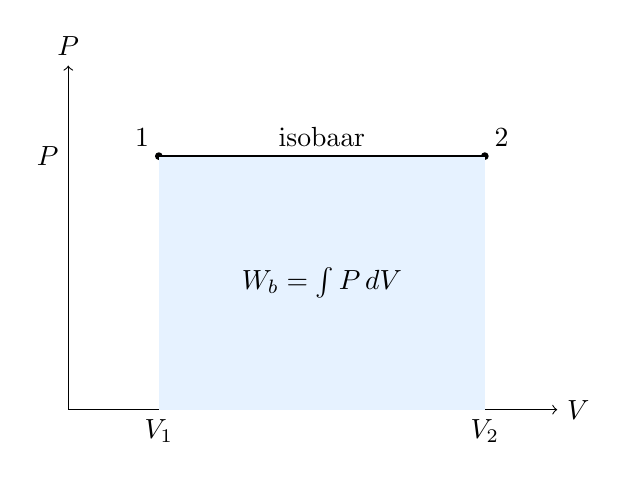
\begin{tikzpicture}[x=1.15cm,y=1.15cm]
        % axes
        \draw[->] (0,0) -- (5.4,0) node[right] {$V$};
        \draw[->] (0,0) -- (0,3.8) node[above] {$P$};

        % isobaric line
        \draw[thick] (1.0,2.8) -- (4.6,2.8);
        \node[above] at (2.8,2.8) {isobaar};

        % states
        \fill (1.0,2.8) circle (1.4pt);
        \fill (4.6,2.8) circle (1.4pt);
        \node[above left] at (1.0,2.8) {1};
        \node[above right] at (4.6,2.8) {2};

        % work area shading
        \fill[lightblue] (1.0,0) rectangle (4.6,2.8);
        \draw[thick] (1.0,2.8) -- (4.6,2.8);
        \node at (2.8,1.4) {$W_b=\int P\,dV$};

        % labels
        \node[below] at (1.0,0) {$V_1$};
        \node[below] at (4.6,0) {$V_2$};
        \node[left] at (0,2.8) {$P$};
    \end{tikzpicture}
    \caption{Interpretatie van grensverplaatsingsarbeid als oppervlakte onder de $P$-$V$ curve.}
\end{figure}

\subsection*{Voorbeeldoefening: isobare expansie in zuiger-cilinder}
        	\textbf{Gegeven:} Een gas in een zuiger-cilinder ondergaat een isobare expansie bij $P=200\,\mathrm{kPa}$. Het volume verandert van $V_1=0{,}10\,\mathrm{m^3}$ naar $V_2=0{,}25\,\mathrm{m^3}$.

        	\textbf{Gevraagd:} Bepaal de grensverplaatsingsarbeid $W_b$ (arbeid door het systeem).

        	\textbf{Oplossing:}
Bij isobaar proces geldt:
\[
W_b=P\,(V_2-V_1)=200\times 10^3\,(0{,}25-0{,}10)=200\times 10^3\cdot 0{,}15=3{,}0\times 10^4\,\mathrm{J}
\]
Dus $\boxed{W_b=30\,\mathrm{kJ}}$ (positief: arbeid geleverd door het gas).

\section{De Eerste Hoofdwet voor Open Systemen (Controlevolumes)}
Bij open systemen stroomt massa de grenzen over. Massa draagt energie met zich mee (interne energie $u$, kinetische energie $V^2/2$ en potentiële energie $gz$). Daarnaast is er energie nodig om de massa in of uit het systeem te duwen tegen de heersende druk in. Deze mechanische energie noemen we stromingsarbeid of flow work ($W_{flow} = Pv$).

Om de thermodynamische analyse van open systemen te vereenvoudigen, combineren we de interne energie $u$ en de stromingsarbeid $Pv$ in een nieuwe eigenschap: enthalpie ($h$).
\[
h = u + Pv
\]
Enthalpie vertegenwoordigt dus de microscopische energie van een fluïdum plus de energie die nodig is om het fluïdum te laten stromen.

De energiebalans voor een algemeen stromingsproces is:
\[
\dot{Q}_{in} + \dot{W}_{in} + \sum \dot{m}_{in} \theta_{in} = \dot{Q}_{uit} + \dot{W}_{uit} + \sum \dot{m}_{uit} \theta_{uit} + \frac{dE_{sys}}{dt}
\]
Waarbij $\theta$ de totale energie per eenheid massa van de stromende vloeistof is: $\theta = h + \frac{V^2}{2} + gz$.

Voor een stationair stromingsproces (steady-flow), waarbij de eigenschappen in het controlevolume niet veranderen met de tijd ($dE_{sys}/dt = 0$) en de in- en uitgaande massastromen gelijk zijn ($\dot{m}_{in} = \dot{m}_{uit} = \dot{m}$), vereenvoudigt dit tot:
\[
\dot{Q} - \dot{W} = \dot{m} \left[ (h_2 - h_1) + \frac{V_2^2 - V_1^2}{2} + g(z_2 - z_1) \right]
\]
Hierbij staat punt 1 voor de inlaat en punt 2 voor de uitlaat. In veel apparaten, zoals nozzles en diffusers, zijn warmte en arbeid verwaarloosbaar, en balanceert de verandering in enthalpie direct de verandering in kinetische energie.

\begin{figure}[H]
    \centering
    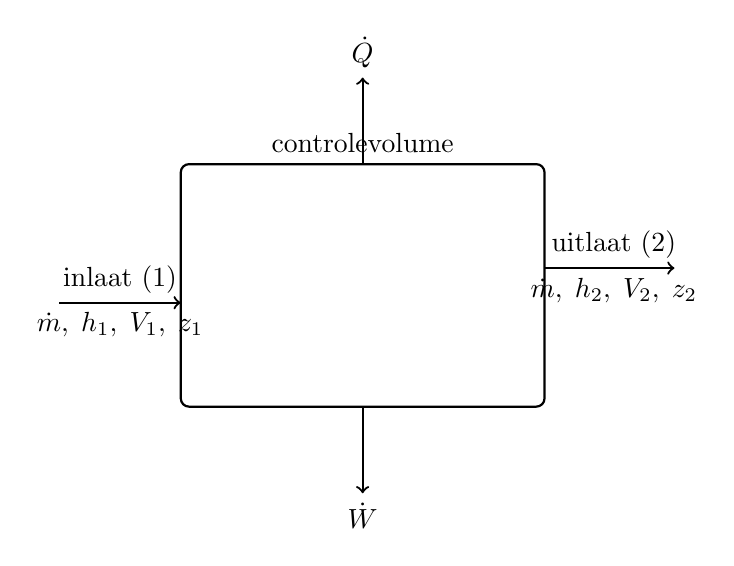
\begin{tikzpicture}[x=1.1cm,y=1.1cm]
        % control volume box
        \draw[thick,rounded corners=3pt] (1.2,0.4) rectangle (5.4,3.2);
        \node at (3.3,3.45) {controlevolume};

        % inlet
        \draw[thick,->] (-0.2,1.6) -- (1.2,1.6);
        \node[above] at (0.5,1.6) {inlaat (1)};
        \node[below] at (0.5,1.6) {$\dot{m},\;h_1,\;V_1,\;z_1$};

        % outlet
        \draw[thick,->] (5.4,2.0) -- (6.9,2.0);
        \node[above] at (6.2,2.0) {uitlaat (2)};
        \node[below] at (6.2,2.0) {$\dot{m},\;h_2,\;V_2,\;z_2$};

        % heat/work
        \draw[thick,->] (3.3,0.4) -- (3.3,-0.6);
        \node[below] at (3.3,-0.6) {$\dot{W}$};
        \draw[thick,->] (3.3,3.2) -- (3.3,4.2);
        \node[above] at (3.3,4.2) {$\dot{Q}$};
    \end{tikzpicture}
    \caption{Schema van een controlevolume met energiestromen via warmte, arbeid en massastromen.}
\end{figure}

\subsection*{Voorbeeldoefening: nozzle (enthalpie naar snelheid)}
        	\textbf{Gegeven:} Een nozzle werkt stationair, adiabatisch ($\dot{Q}\approx 0$) en zonder as-arbeid ($\dot{W}\approx 0$). De snelheidsverandering is dominant, hoogteverschil verwaarloosbaar. Het massadebiet is $\dot{m}=0{,}50\,\mathrm{kg/s}$. Inlaat: $V_1\approx 20\,\mathrm{m/s}$. Uitlaat: $V_2\approx 220\,\mathrm{m/s}$.

        	\textbf{Gevraagd:} Bepaal de vereiste enthalpiedaling $\Delta h=h_2-h_1$.

        	\textbf{Oplossing:}
Met $\dot{Q}-\dot{W}=\dot{m}\left[(h_2-h_1)+\frac{V_2^2-V_1^2}{2}\right]$ en $\dot{Q}\approx\dot{W}\approx 0$:
\[
h_2-h_1\approx -\frac{V_2^2-V_1^2}{2}
\]
\[
V_2^2-V_1^2=220^2-20^2=48400-400=48000\,\mathrm{m^2/s^2}
\]
\[
\Delta h\approx -\frac{48000}{2}=-24000\,\mathrm{J/kg}=-24\,\mathrm{kJ/kg}
\]
Dus de nozzle “zet” ongeveer $\boxed{24\,\mathrm{kJ/kg}}$ enthalpie om in kinetische energie.

\chapter{Eigenschappen van Zuivere Stoffen}
Om de energiebalansen op te lossen, moeten we de waarden van $u$, $h$ en $v$ kunnen bepalen. Stoffen zoals water of koelmiddel (R-134a) gedragen zich complexer dan ideale gassen vanwege faseovergangen. Een zuivere stof heeft een uniforme chemische samenstelling.

\section{Fasen en Faseverandering}
We kennen drie hoofdfasen: vaste stof, vloeistof en gas. De thermodynamica van faseverandering is rijk aan terminologie:
\begin{itemize}
    \item \textbf{Gecomprimeerde vloeistof (subcooled liquid):} Vloeistof die niet op het punt staat te verdampen (bijv. water bij 20°C en 1 atm).
    \item \textbf{Verzadigde vloeistof (saturated liquid):} Vloeistof die op het punt staat te koken. Elke toevoeging van warmte zorgt voor dampvorming.
    \item \textbf{Verzadigde damp (saturated vapor):} Damp die op het punt staat te condenseren. Elke onttrekking van warmte zorgt voor druppelvorming.
    \item \textbf{Oververhitte damp (superheated vapor):} Damp die niet op het punt staat te condenseren (bijv. stoom bij 300°C en 1 atm).
\end{itemize}
\textbf{Verzadigingstemperatuur ($T_{sat}$) en -druk ($P_{sat}$):} Bij een gegeven druk is er een specifieke temperatuur waarbij een zuivere stof kookt. Water kookt bijvoorbeeld bij 100°C bij 1 atm, maar bij een lagere temperatuur op grote hoogte waar de druk lager is.

\section{Eigenschapsdiagrammen en Tabellen}
De relaties tussen eigenschappen worden gevisualiseerd in $T-v$, $P-v$ en $P-T$ diagrammen. Op een $T-v$ diagram zien we een karakteristieke "koepel" (de verzadigingskoepel):
\begin{itemize}
    \item De linkerzijde van de koepel is de verzadigde vloeistoflijn.
    \item De rechterzijde is de verzadigde damplijn.
    \item Het punt waar de lijnen samenkomen is het kritieke punt. Boven de kritieke temperatuur en druk is er geen duidelijk onderscheid meer tussen vloeistof en damp.
\end{itemize}

\begin{figure}[H]
    \centering
    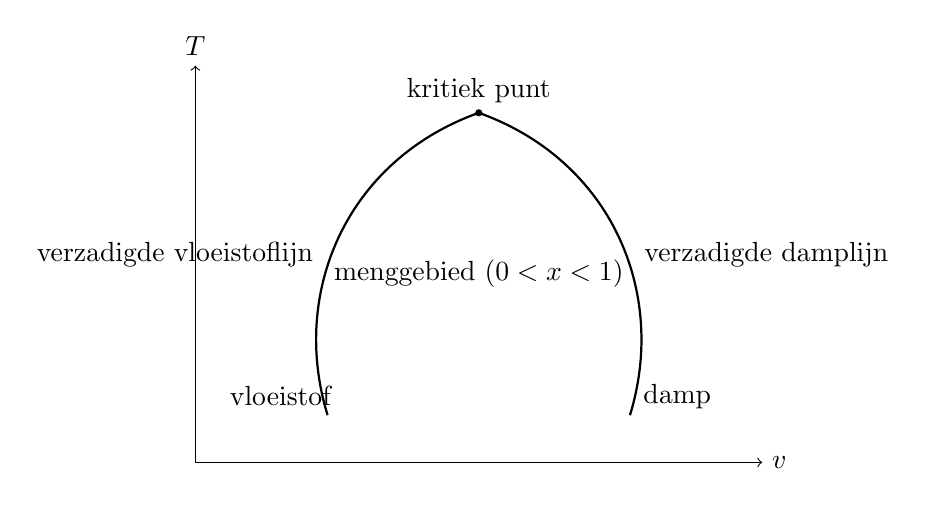
\begin{tikzpicture}[x=1.2cm,y=1.2cm]
        % axes
        \draw[->] (0,0) -- (6.0,0) node[right] {$v$};
        \draw[->] (0,0) -- (0,4.2) node[above] {$T$};

        % saturation dome (stylized)
        \draw[thick] (1.4,0.5) .. controls (1.0,1.8) and (1.6,3.2) .. (3.0,3.7);
        \draw[thick] (4.6,0.5) .. controls (5.0,1.8) and (4.4,3.2) .. (3.0,3.7);
        \node[above] at (3.0,3.7) {kritiek punt};
        \fill (3.0,3.7) circle (1.3pt);

        % labels
        \node[left] at (1.35,2.2) {verzadigde
vloeistoflijn};
        \node[right] at (4.65,2.2) {verzadigde
damplijn};
        \node at (3.0,2.0) {menggebied
($0<x<1$)};
        \node at (0.9,0.7) {vloeistof};
        \node at (5.1,0.7) {damp};
    \end{tikzpicture}
    \caption{Schematisch $T$-$v$ diagram met verzadigingskoepel en kwaliteit $x$ in het menggebied.}
\end{figure}

\begin{figure}[H]
    \centering
    \includegraphics[width=0.5\textwidth]{assets/wikipedia/phase_diagram_water_960.png}
    \caption{$P$-$T$ fasediagram van water (log-schaal in druk), met tripelpunt en kritisch punt.\;\scriptsize Bron: Cmglee, CC BY-SA 3.0, via Wikimedia Commons (\url{https://commons.wikimedia.org/wiki/File:Phase_diagram_of_water.svg}).}
\end{figure}
Onder de koepel bevindt zich het menggebied, waar vloeistof en damp in evenwicht samen bestaan. In dit gebied zijn druk en temperatuur afhankelijk van elkaar. Om de toestand vast te leggen, gebruiken we de kwaliteit of dampfractie $x$, gedefinieerd als de verhouding van de massa damp tot de totale massa van het mengsel:
\[
x = \frac{m_{damp}}{m_{totaal}}
\]
De waarde van $x$ loopt van 0 (verzadigde vloeistof) tot 1 (verzadigde damp). De eigenschappen van het mengsel worden berekend als een gewogen gemiddelde:
\[
y_{gem} = y_f + x \cdot y_{fg}
\]
Waarbij $y$ staat voor een specifieke eigenschap ($v$, $u$, of $h$). $y_f$ is de waarde voor verzadigde vloeistof en $y_{fg}$ is het verschil tussen verzadigde damp en vloeistof ($y_g - y_f$). Deze waarden vinden we in thermodynamische tabellen.

\subsection*{Voorbeeldoefening: kwaliteit en mengseleigenschap}
                    	\textbf{Gegeven:} In een verzadigd mengsel geldt bij een bepaalde druk: $h_f=500\,\mathrm{kJ/kg}$ en $h_g=2700\,\mathrm{kJ/kg}$. De gemeten enthalpie van het mengsel is $h=1600\,\mathrm{kJ/kg}$.

                        	\textbf{Gevraagd:} Bepaal de kwaliteit $x$.

                        	\textbf{Oplossing:}
We gebruiken $h=h_f+x(h_g-h_f)$:
\[
x=\frac{h-h_f}{h_g-h_f}=\frac{1600-500}{2700-500}=\frac{1100}{2200}=0{,}50
\]
Dus $\boxed{x=0{,}50}$: de massa bestaat voor 50\% uit damp.

\section{De Ideale Gaswet}
Voor gassen bij hoge temperatuur en lage druk (ten opzichte van hun kritieke waarden) zijn de intermoleculaire krachten verwaarloosbaar klein. Onder deze omstandigheden kunnen we de Ideale Gaswet gebruiken:
\[
Pv = RT
\]
\symW{R}{specifieke gasconstante}{J/(kg\,K)}
\symW{v}{specifiek volume}{m$^3$/kg}
Hierin is $R$ de specifieke gasconstante, die verschilt per gas ($R = R_u / M$, met $R_u = 8.314 \, kJ/kmol\cdot K$ de universele gasconstante en $M$ de molaire massa).

Een belangrijke eigenschap van ideale gassen is dat de interne energie en enthalpie enkel afhangen van de temperatuur ($u = u(T)$ en $h = h(T)$). Dit leidt tot de definities van de soortelijke warmten:
\begin{itemize}
    \item $c_v = (\frac{\partial u}{\partial T})_v = \frac{du}{dT}$ $\rightarrow$ $\Delta u = c_v \Delta T$ (voor constante $c_v$)
    \item $c_p = (\frac{\partial h}{\partial T})_p = \frac{dh}{dT}$ $\rightarrow$ $\Delta h = c_p \Delta T$ (voor constante $c_p$)
\end{itemize}

\symW{c_v}{soortelijke warmte bij constant volume}{kJ/(kg\,K)}
\symW{c_p}{soortelijke warmte bij constant druk}{kJ/(kg\,K)}

De verhouding $k = c_p / c_v$ is de specifieke warmteverhouding, die een rol speelt bij adiabatische processen van ideale gassen ($Pv^k = C$).

Indien een gas te sterk afwijkt van ideaal gedrag (bijvoorbeeld bij hoge druk), gebruiken we de compressibiliteitsfactor $Z$ ($Pv = ZRT$) of complexere toestandsvergelijkingen zoals van der Waals of Beattie-Bridgeman.

\chapter{De Tweede Hoofdwet en Entropie}
De Eerste Wet stelt dat energie behouden blijft, maar zegt niets over de richting van een proces. Een kop koffie koelt af in een kamer, maar wordt nooit spontaan warmer door energie uit de kamerlucht te onttrekken, hoewel dit de eerste wet niet zou schenden. Dit inzicht leidt tot de Tweede Hoofdwet van de Thermodynamica.

\section{Kelvin-Planck en Clausius}
De Tweede Wet wordt vaak geformuleerd in termen van onmogelijkheden:
\begin{itemize}
    \item \textbf{Kelvin-Planck stelling:} Het is onmogelijk om een apparaat te bouwen dat in een cyclus werkt en warmte uit één enkel reservoir ontvangt en dit volledig omzet in arbeid. Met andere woorden: geen enkele warmtemotor kan een thermisch rendement van 100\% hebben. Een warmtemotor moet een deel van de warmte afstaan aan een koud reservoir ("waste heat").
    \item \textbf{Clausius stelling:} Het is onmogelijk om een apparaat te bouwen dat warmte van een koud medium naar een warmer medium verplaatst zonder toevoeging van arbeid. Dit betekent dat een koelkast niet "gratis" kan werken; er is altijd een compressor nodig die arbeid verbruikt.
\end{itemize}

\section{Entropie}
Om de Tweede Wet kwantitatief te maken, introduceerde Clausius het concept entropie ($S$). Entropie kan worden gezien als een maat voor moleculaire wanorde of de "kwaliteit" van energie. Hoe hoger de entropie, hoe minder bruikbaar de energie is voor arbeid.
De verandering in entropie $dS$ wordt gedefinieerd als $dQ/T$ voor een intern reversibel proces. Voor elk proces geldt het principe van toename van entropie:
\[
dS \ge \frac{\delta Q}{T}
\]
Voor een geïsoleerd systeem betekent dit dat de entropie altijd toeneemt (bij irreversibele, echte processen) of gelijk blijft (bij reversibele, ideale processen), maar nooit afneemt ($\Delta S_{gen} \ge 0$). Irreversibiliteiten zoals wrijving, menging en warmteoverdracht over een eindig temperatuurverschil genereren entropie.

\subsection*{Belangrijke Formules}
\begingroup
\setlength{\tabcolsep}{6pt}
\renewcommand{\arraystretch}{1.35}
\[
\begin{array}{@{}lcl@{}}
        	\textbf{Clausius-ongelijkheid} &:& \Delta S \ge \displaystyle\int \frac{\delta Q}{T}\\
        	\textbf{Intern reversibel} &:& ds=\frac{\delta q_{rev}}{T}\\
        	\textbf{Entropiebalans (gesloten)} &:& \Delta S = \displaystyle\int \frac{\delta Q}{T_{grens}} + S_{gen}\\
        	\textbf{Entropiebalans (stationair CV)} &:& \dot{S}_{gen}=\sum \dot{m}\,s_{out}-\sum \dot{m}\,s_{in}-\sum \frac{\dot{Q}_k}{T_k}\\
        	\textbf{Ideaal gas} &:& \Delta s=c_p\ln\left(\frac{T_2}{T_1}\right)-R\ln\left(\frac{P_2}{P_1}\right)\\
        	\textbf{Incompressibel (c const.)} &:& \Delta s=c\ln\left(\frac{T_2}{T_1}\right)\\
\end{array}
\]
\symW{s}{specifieke entropie}{kJ/(kg\,K)}
\endgroup

\subsection*{Omkeerbaar vs. onomkeerbaar (intuïtie)}
Een proces is \textbf{omkeerbaar} als het (idealiter) zonder netto sporen in systeem én omgeving terug te draaien is. In de praktijk is dit een limietgeval.

Typische bronnen van \textbf{onomkeerbaarheid}:
\begin{itemize}
    \item wrijving (mechanisch of intern in het fluïdum)
    \item mengen van stoffen/temperaturen
    \item warmteoverdracht bij eindig $\Delta T$
    \item smoren (throttling) door kleppen/vernauwingen
\end{itemize}
Onomkeerbaar $\Rightarrow S_{gen}>0$.

\begin{figure}[H]
    \centering
    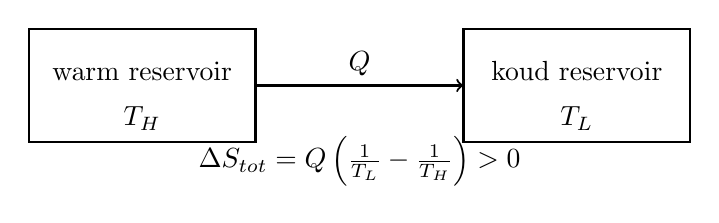
\begin{tikzpicture}[x=1.2cm,y=1.2cm]
        \draw[thick] (0,0) rectangle (2.4,1.2);
        \draw[thick] (4.6,0) rectangle (7.0,1.2);
        \node at (1.2,0.75) {warm reservoir};
        \node at (1.2,0.25) {$T_H$};
        \node at (5.8,0.75) {koud reservoir};
        \node at (5.8,0.25) {$T_L$};
        \draw[thick,->] (2.4,0.6) -- (4.6,0.6);
        \node[above] at (3.5,0.6) {$Q$};
        \node at (3.5,-0.2) {$\Delta S_{tot}=Q\left(\frac{1}{T_L}-\frac{1}{T_H}\right)>0$};
    \end{tikzpicture}
    \caption{Warmteoverdracht bij eindig $\Delta T$ is onomkeerbaar en genereert entropie.}
\end{figure}

\subsection*{Voorbeeldoefening: entropieverandering bij opwarming (incompressibel)}
        	\textbf{Gegeven:} $m=2{,}0\,\mathrm{kg}$ water wordt opgewarmd van $T_1=20^\circ\mathrm{C}$ naar $T_2=80^\circ\mathrm{C}$. Neem $c\approx 4{,}18\,\mathrm{kJ/(kg\cdot K)}$.

        	\textbf{Gevraagd:} Bepaal $\Delta S$ van het water.

        	\textbf{Oplossing:}
Zet om naar Kelvin: $T_1=293\,\mathrm{K}$ en $T_2=353\,\mathrm{K}$.
\[
\Delta S=m c\ln\left(\frac{T_2}{T_1}\right)=2{,}0\cdot 4{,}18\ln\left(\frac{353}{293}\right)\approx 1{,}55\,\mathrm{kJ/K}
\]
Dus $\boxed{\Delta S\approx 1{,}55\,\mathrm{kJ/K}}$.

\subsection*{Voorbeeldoefening: entropieproductie bij warmteoverdracht tussen reservoirs}
        	\textbf{Gegeven:} $Q=500\,\mathrm{kJ}$ stroomt van $T_H=600\,\mathrm{K}$ naar $T_L=300\,\mathrm{K}$.

        	\textbf{Gevraagd:} Bepaal $\Delta S_{tot}$ en $S_{gen}$.

        	\textbf{Oplossing:}
\[
\Delta S_{warm}=-\frac{Q}{T_H}=-\frac{500}{600}=-0{,}833\,\mathrm{kJ/K},\qquad
\Delta S_{koud}=+\frac{Q}{T_L}=+\frac{500}{300}=1{,}667\,\mathrm{kJ/K}
\]
\[
\Delta S_{tot}=\Delta S_{warm}+\Delta S_{koud}=0{,}834\,\mathrm{kJ/K}
\]
Omdat dit proces onomkeerbaar is, geldt $S_{gen}=\Delta S_{tot}>0$.

\section{Isentropische Processen en Efficiëntie}
Een proces dat zowel adiabatisch ($Q=0$) als reversibel ($S_{gen}=0$) is, wordt isentroop genoemd. Hierbij blijft de entropie constant ($\Delta s = 0$). Isentropische processen dienen als het ideale vergelijkingsmodel voor machines zoals turbines, compressoren en nozzles.

De isentropische efficiëntie is een maat voor hoe dicht een werkelijk apparaat de ideale prestatie benadert:
\begin{itemize}
    \item Voor een turbine: $\eta_T = \frac{\text{Werkelijke Arbeid}}{\text{Isentropische Arbeid}} \approx \frac{h_1 - h_{2a}}{h_1 - h_{2s}}$
    \item Voor een compressor: $\eta_C = \frac{\text{Isentropische Arbeid}}{\text{Werkelijke Arbeid}} \approx \frac{h_{2s} - h_1}{h_{2a} - h_1}$
\end{itemize}

\chapter{Thermodynamische Cycli}
De toepassing van thermodynamica culmineert in de analyse van cycli voor krachtcentrales en koelmachines.

\section{De Carnot Cyclus}
Dit is de meest efficiënte theoretische cyclus die mogelijk is tussen twee temperatuurlimieten. Hij bestaat uit vier volledig reversibele processen:
\begin{enumerate}
    \item Isotherme expansie (warmtetoevoer bij $T_H$)
    \item Adiabatische expansie (temperatuurdaling tot $T_L$)
    \item Isotherme compressie (warmteafvoer bij $T_L$)
    \item Adiabatische compressie (temperatuurstijging tot $T_H$)
\end{enumerate}
Het thermisch rendement van een Carnot-motor hangt enkel af van de absolute temperaturen van de reservoirs:
\[
\eta_{th, Carnot} = 1 - \frac{T_L}{T_H}
\]
Dit stelt de theoretische bovengrens voor elke warmtemotor. Om het rendement te verhogen, moet men $T_H$ verhogen of $T_L$ verlagen.

\subsection*{$T$-$s$ diagram van de Carnot-cyclus (schematisch)}
Voor een intern reversibele cyclus geldt $\delta q_{rev}=T\,ds$. Daardoor geeft de oppervlakte in het $T$-$s$ diagram een directe interpretatie van warmte en (via de energiebalans over een cyclus) netto arbeid.

\begin{figure}[H]
    \centering
    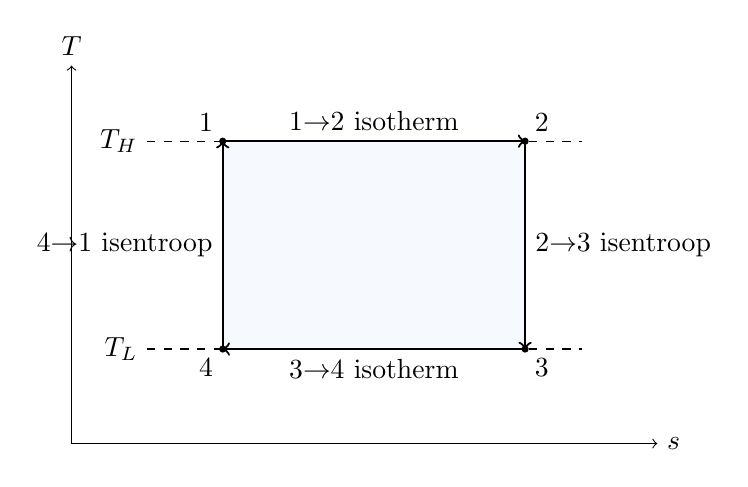
\begin{tikzpicture}[x=1.2cm,y=1.2cm]
        \draw[->] (0,0) -- (6.2,0) node[right] {$s$};
        \draw[->] (0,0) -- (0,4.0) node[above] {$T$};

        \draw[dashed] (0.8,3.2) -- (5.4,3.2);
        \draw[dashed] (0.8,1.0) -- (5.4,1.0);
        \node[left] at (0.8,3.2) {$T_H$};
        \node[left] at (0.8,1.0) {$T_L$};

        \fill[lightblue,opacity=0.35] (1.6,1.0) rectangle (4.8,3.2);
        \draw[thick,->] (1.6,3.2) -- (4.8,3.2) node[midway,above] {1$\to$2 isotherm};
        \draw[thick,->] (4.8,3.2) -- (4.8,1.0) node[midway,right] {2$\to$3 isentroop};
        \draw[thick,->] (4.8,1.0) -- (1.6,1.0) node[midway,below] {3$\to$4 isotherm};
        \draw[thick,->] (1.6,1.0) -- (1.6,3.2) node[midway,left] {4$\to$1 isentroop};

        \fill (1.6,3.2) circle (1.3pt) node[above left] {1};
        \fill (4.8,3.2) circle (1.3pt) node[above right] {2};
        \fill (4.8,1.0) circle (1.3pt) node[below right] {3};
        \fill (1.6,1.0) circle (1.3pt) node[below left] {4};
    \end{tikzpicture}
    \caption{$T$-$s$ diagram van de reversibele Carnot-cyclus.}
\end{figure}

\subsection*{Omgekeerde Carnot (koelkast/warmtepomp) en COP}
Voor koelmachines gebruiken we de \textbf{Coefficient of Performance (COP)}:
\[
\mathrm{COP}_{\mathrm{koelkast}}=\frac{Q_L}{W_{in}},\qquad
\mathrm{COP}_{\mathrm{warmtepomp}}=\frac{Q_H}{W_{in}}
\]
Voor de reversibele (Carnot) limiet volgt:
\[
\mathrm{COP}_{\mathrm{koelkast,C}}=\frac{T_L}{T_H-T_L},\qquad
\mathrm{COP}_{\mathrm{warmtepomp,C}}=\frac{T_H}{T_H-T_L}
\]

\subsection*{Voorbeeldoefening: COP van een Carnot-koelkast}
	\textbf{Gegeven:} Een koelkast werkt ideaal tussen $T_L=270\,\mathrm{K}$ en $T_H=300\,\mathrm{K}$.

	\textbf{Gevraagd:} Bepaal $\mathrm{COP}_{\mathrm{koelkast,C}}$.

	\textbf{Oplossing:}
\[
\mathrm{COP}_{\mathrm{koelkast,C}}=\frac{270}{300-270}=9
\]
Dus $\boxed{\mathrm{COP}\approx 9}$ (bovengrens).

\section{Otto en Diesel Cycli}
Dit zijn de geïdealiseerde modellen voor interne verbrandingsmotoren (resp. benzine en diesel).
\begin{itemize}
    \item \textbf{Otto-cyclus:} Bestaat uit isentrope (waarbij entropy $s$ constant is) compressie, isochore (waarbij volume $V$ constant is) warmtetoevoer (ontsteking), isentrope expansie (arbeidsslag) en isochore warmteafvoer. Het rendement is een functie van de compressieverhouding $r$ en de specifieke warmteverhouding $k$: $\eta = 1 - r^{1-k}$.
    \item \textbf{Diesel-cyclus:} Verschilt van Otto doordat de verbranding trager verloopt; dit wordt gemodelleerd als warmtetoevoer bij constante druk (isobaar) gedurende een deel van de expansieslag.
\end{itemize}

\begin{figure}[H]
    \centering
    \includegraphics[width=0.6\textwidth]{assets/otto_cycle.png}
    \caption{P-V diagram van de Otto-cyclus.}
    \label{fig:otto}
\end{figure}

\section{Rankine Cyclus}
Dit is de basiscyclus voor stoomkrachtcentrales. De werkvloeistof (water) ondergaat faseveranderingen:
\begin{enumerate}
    \item \textbf{Pomp:} Verhoogt de druk van vloeibaar water (isentrope compressie).
    \item \textbf{Ketel (Boiler):} Verdampt het water tot stoom bij constante druk (isobare warmtetoevoer).
    \item \textbf{Turbine:} De stoom expandeert en levert arbeid (isentrope expansie).
    \item \textbf{Condensor:} De stoom condenseert terug naar vloeistof bij constante druk (isobare warmteafvoer).
\end{enumerate}

\begin{figure}[H]
    \centering
    \includegraphics[width=0.8\textwidth]{assets/wikipedia/rankine_cycle_layout_cc0_1024.png}
    \caption{Schema van de Rankine-cyclus.\;\scriptsize Bron: D. Ilyin (vectorisatie), CC0, via Wikimedia Commons (\url{https://commons.wikimedia.org/wiki/File:Rankine_cycle_layout.svg}).}
    \label{fig:rankine}
\end{figure}

\section{Dampcompressie Koelcyclus}
Dit is de cyclus die gebruikt wordt in koelkasten en airconditioners. Het is in wezen een omgekeerde warmtemotor, bestaande uit een compressor, condensor, expansieventiel en verdamper. Een bijzonderheid is het expansieventiel, waar vloeistof door een vernauwing stroomt. Dit is een onomkeerbaar proces waarbij de druk sterk daalt en een deel van de vloeistof verdampt ("flashing"), wat leidt tot een sterke temperatuurdaling. Dit proces wordt als isenthalpisch ($h \approx \text{constant}$) beschouwd.

\subsection*{COP (praktisch)}
In de praktijk wordt de COP vaak bepaald uit vermogens:
\[
\mathrm{COP}=\frac{\dot{Q}_L}{\dot{W}_{in}}
\]
waar $\dot{Q}_L$ de warmte is die uit de koude ruimte onttrokken wordt (verdamper) en $\dot{W}_{in}$ het compressor-/elektrisch vermogen.

\subsection*{Diagram: dampcompressiecyclus op $T$-$s$ (schematisch)}
De smoring (3$\to$4) is typisch \textbf{onomkeerbaar} en verhoogt de entropie.
\begin{figure}[H]
    \centering
    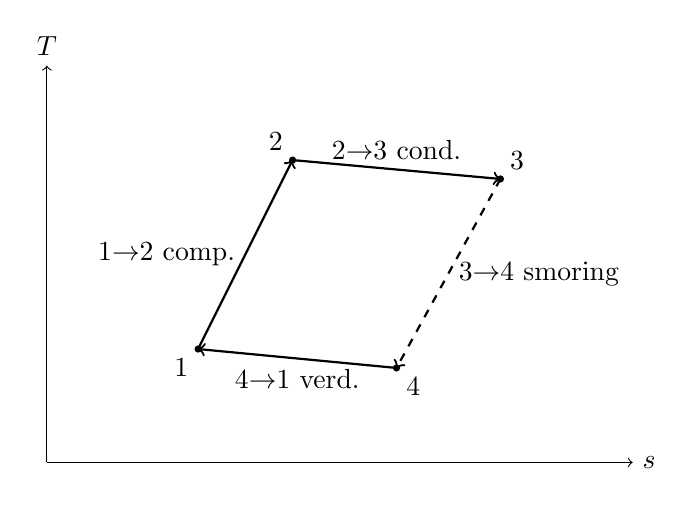
\begin{tikzpicture}[x=1.2cm,y=1.2cm]
        \draw[->] (0,0) -- (6.2,0) node[right] {$s$};
        \draw[->] (0,0) -- (0,4.2) node[above] {$T$};

        \coordinate (p1) at (1.6,1.2);
        \coordinate (p2) at (2.6,3.2);
        \coordinate (p3) at (4.8,3.0);
        \coordinate (p4) at (3.7,1.0);

        \draw[thick,->] (p1) -- (p2) node[midway,left] {1$\to$2 comp.};
        \draw[thick,->] (p2) -- (p3) node[midway,above] {2$\to$3 cond.};
        \draw[thick,->,dashed] (p3) -- (p4) node[midway,right] {3$\to$4 smoring};
        \draw[thick,->] (p4) -- (p1) node[midway,below] {4$\to$1 verd.};

        \fill (p1) circle (1.3pt) node[below left] {1};
        \fill (p2) circle (1.3pt) node[above left] {2};
        \fill (p3) circle (1.3pt) node[above right] {3};
        \fill (p4) circle (1.3pt) node[below right] {4};
    \end{tikzpicture}
    \caption{Schematische dampcompressiecyclus in een $T$-$s$ diagram (smoring is onomkeerbaar).}
\end{figure}

\subsection*{Voorbeeldoefening: COP uit vermogens}
                    	\textbf{Gegeven:} Een koelkast onttrekt $\dot{Q}_L=1{,}8\,\mathrm{kW}$ en de compressor verbruikt $\dot{W}_{in}=0{,}60\,\mathrm{kW}$.

                    	\textbf{Gevraagd:} Bepaal de COP.

                    	\textbf{Oplossing:}
\[
\mathrm{COP}=\frac{1{,}8}{0{,}60}=3{,}0
\]
Dus $\boxed{\mathrm{COP}=3{,}0}$.

\section{Omkeerbare en onomkeerbare cycli (concept)}
Onomkeerbaarheid (wrijving, drukverlies, smoring, warmteoverdracht bij eindig $\Delta T$) verhoogt $S_{gen}$ en verlaagt de prestaties t.o.v. de ideale (reversibele) cyclus.
\begin{figure}[H]
    \centering
    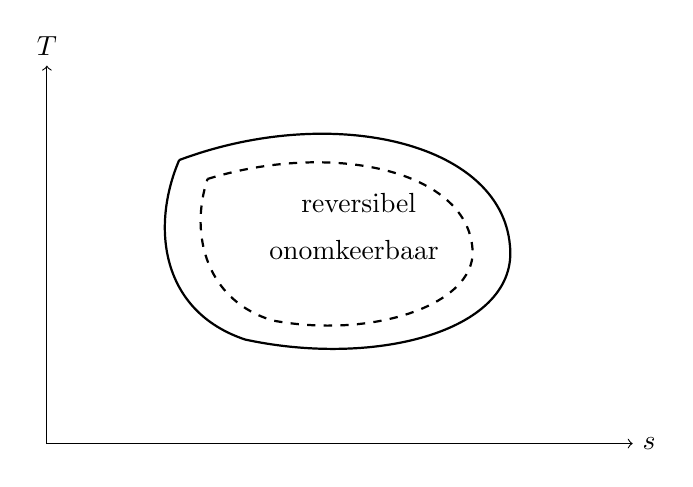
\begin{tikzpicture}[x=1.2cm,y=1.2cm]
        \draw[->] (0,0) -- (6.2,0) node[right] {$s$};
        \draw[->] (0,0) -- (0,4.0) node[above] {$T$};

        % reversible loop
        \draw[thick] (1.4,3.0) .. controls (3.0,3.6) and (4.8,3.2) .. (4.9,2.1)
                     .. controls (5.0,1.2) and (3.5,0.8) .. (2.1,1.1)
                     .. controls (1.2,1.4) and (1.1,2.3) .. (1.4,3.0);
        \node at (3.3,2.55) {reversibel};

        % irreversible loop
        \draw[thick,dashed] (1.7,2.8) .. controls (3.0,3.2) and (4.4,2.9) .. (4.5,2.1)
                            .. controls (4.6,1.5) and (3.5,1.1) .. (2.4,1.3)
                            .. controls (1.7,1.5) and (1.5,2.2) .. (1.7,2.8);
        \node at (3.25,2.05) {onomkeerbaar};
    \end{tikzpicture}
    \caption{Conceptueel: onomkeerbaarheid verkleint de ingesloten oppervlakte in $T$-$s$ en verlaagt de cyclusprestatie.}
\end{figure}

\chapter{Warmteoverdracht Mechanismen}
Thermodynamica vertelt ons hoeveel warmte wordt overgedragen om van de ene toestand naar de andere te gaan, maar zegt niets over hoe lang dat duurt. Warmteoverdracht is de wetenschap die de snelheid van energie-overdracht berekent, gedreven door een temperatuurverschil $\Delta T$. Er zijn drie fundamentele mechanismen.
\subsection*{Belangrijke Formules}
\begingroup
\setlength{\tabcolsep}{6pt}
\renewcommand{\arraystretch}{1.35}
\[
\begin{array}{@{}lcl@{}}
                    	\textbf{Fourier (1D)} &:& \dot{Q}=-kA\,\dfrac{dT}{dx}\\
                    	\textbf{Vlakke wand (stationair)} &:& \dot{Q}=kA\,\dfrac{T_1-T_2}{L}\\
                    	\textbf{Warmteweerstand (vlak)} &:& R_{cond}=\dfrac{L}{kA}\\
                    	\textbf{Weerstanden in serie} &:& R_{tot}=\sum_i \dfrac{L_i}{k_i A}\\
                    	\textbf{Weerstandsnetwerk} &:& \dot{Q}=
        \dfrac{T_{hot}-T_{cold}}{R_{tot}}\\
\end{array}
\]
\endgroup

\IfFileExists{assets/cengel_conduction_plane_wall.png}{%
\begin{figure}[H]
    \centering
    \includegraphics[width=0.75\linewidth]{assets/cengel_conduction_plane_wall.png}
    \caption{Figuur (uit eigen bronbestand): stationaire conductie door een vlakke wand.}
\end{figure}
}{}

\subsection*{Voorbeeldoefening: stationaire geleiding door een vlakke wand}
                        	\textbf{Gegeven:} Een vlakke wand met $k=0{,}80\,\mathrm{W/(m\cdot K)}$, oppervlakte $A=10\,\mathrm{m^2}$ en dikte $L=0{,}20\,\mathrm{m}$. De warme zijde is $T_1=60^\circ\mathrm{C}$ en de koude zijde $T_2=40^\circ\mathrm{C}$.

                                	\textbf{Gevraagd:} Bepaal $\dot{Q}$ en schets $T(x)$.

                                	\textbf{Oplossing:}
\[
\dot{Q}=kA\frac{T_1-T_2}{L}=0{,}80\cdot 10\cdot\frac{20}{0{,}20}=800\,\mathrm{W}
\]
Het temperatuurprofiel is lineair (constante $k$, 1D, stationair).

\begin{figure}[H]
    \centering
    \begin{tikzpicture}[x=1.2cm,y=1.2cm]
        % axes
        \draw[->] (0,0) -- (5.2,0) node[right] {$x$};
        \draw[->] (0,0) -- (0,3.2) node[above] {$T$};

        % linear profile
        \draw[thick] (0.8,2.8) -- (4.6,1.2);
        \node[left] at (0.8,2.8) {$T_1$};
        \node[right] at (4.6,1.2) {$T_2$};

        % thickness
        \draw[thin,<->] (0.8,-0.35) -- (4.6,-0.35);
        \node[below] at (2.7,-0.35) {$L$};
    \end{tikzpicture}
    \caption{Lineair $T(x)$-profiel bij stationaire conductie door een vlakke wand.}
\end{figure}

\section{Convectie}
Convectie is de energie-overdracht tussen een vast oppervlak en een aangrenzend stromend fluïdum (gas of vloeistof). Het is een combinatie van geleiding (direct aan het oppervlak) en advectie (macroscopische beweging van de vloeistof die de warmte meevoert).

\IfFileExists{assets/cengel_convection_boundary_layer.png}{%
\begin{figure}[H]
    \centering
    \includegraphics[width=0.78\linewidth]{assets/cengel_convection_boundary_layer.png}
    \caption{Figuur (uit eigen bronbestand): grenslaagconcept bij convectie aan een oppervlak.}
\end{figure}
}{}

De snelheid wordt berekend met de Wet van Newton voor afkoeling:
\[
\dot{Q}_{conv} = h A_s (T_s - T_{\infty})
\]
Hier is $h$ de convectiecoëfficiënt ($W/m^2 \cdot K$). Deze waarde is geen materiaaleigenschap, maar hangt complex af van de stromingscondities (snelheid, turbulentie, viscositeit) en de geometrie.

We onderscheiden:
\begin{itemize}
    \item \textbf{Gedwongen convectie:} De stroming wordt aangedreven door externe middelen zoals een ventilator, pomp of wind. Dit levert doorgaans hoge $h$-waarden op.
    \item \textbf{Natuurlijke (vrije) convectie:} De stroming ontstaat door dichtheidsverschillen als gevolg van temperatuurverschillen in het fluïdum (warme lucht is lichter en stijgt op).
\end{itemize}

\subsection*{Belangrijke Formules}
\begingroup
\setlength{\tabcolsep}{6pt}
\renewcommand{\arraystretch}{1.35}
\[
\begin{array}{@{}lcl@{}}
            \textbf{Newton (convectie)} &:& \dot{Q}=hA\,(T_s-T_\infty)\\
            \textbf{Convectieweerstand} &:& R_{conv}=\dfrac{1}{hA}\\
            \textbf{Lumped capacitance} &:& \dfrac{dT}{dt}=-\dfrac{hA}{mc}\,(T-T_\infty)\\
            \textbf{Oplossing} &:& T(t)=T_\infty+(T_0-T_\infty)e^{-t/\tau},\;\tau=\dfrac{mc}{hA}\\
\end{array}
\]
\endgroup

\subsection*{Voorbeeldoefening: Newton-afkoeling (lumped model)}
        	\textbf{Gegeven:} Een metalen blok met massa $m=2{,}0\,\mathrm{kg}$ en $c=900\,\mathrm{J/(kg\cdot K)}$ koelt af in lucht met $T_\infty=20^\circ\mathrm{C}$. Het effectieve oppervlak is $A=0{,}10\,\mathrm{m^2}$ en $h=10\,\mathrm{W/(m^2\cdot K)}$. Starttemperatuur $T_0=120^\circ\mathrm{C}$.

            	\textbf{Gevraagd:} Bepaal $T$ na $t=10\,\mathrm{min}$.

            	\textbf{Oplossing:}
\[
            	\tau=\frac{mc}{hA}=\frac{2{,}0\cdot 900}{10\cdot 0{,}10}=1800\,\mathrm{s},\qquad t=600\,\mathrm{s}
\]
\[
T(t)=20+(120-20)e^{-600/1800}=20+100e^{-1/3}\approx 91{,}6^\circ\mathrm{C}
\]

\begin{figure}[H]
    \centering
    \begin{tikzpicture}[x=1.2cm,y=1.2cm]
        % axes
        \draw[->] (0,0) -- (5.4,0) node[right] {$t$};
        \draw[->] (0,0) -- (0,3.2) node[above] {$T$};

        % asymptote
        \draw[dashed] (0,0.6) -- (5.1,0.6);
        \node[left] at (0,0.6) {$T_\infty$};

        % exponential curve (schematic)
        \draw[thick] (0.6,2.8) .. controls (1.5,2.2) and (2.4,1.55) .. (3.5,1.05)
                      .. controls (4.3,0.8) and (4.8,0.7) .. (5.1,0.65);
        \node[left] at (0.6,2.8) {$T_0$};
    \end{tikzpicture}
    \caption{Exponentiële afkoeling volgens Newton (lumped capacitance).}
\end{figure}

\section{Straling}
Straling is energie-overdracht via elektromagnetische golven (fotonen). In tegenstelling tot conductie en convectie, heeft straling geen medium nodig; het werkt het efficiëntst in een vacuüm. Alle materie boven het absolute nulpunt zendt thermische straling uit.

\IfFileExists{assets/cengel_radiation_exchange.png}{%
\begin{figure}[H]
    \centering
    \includegraphics[width=0.78\linewidth]{assets/cengel_radiation_exchange.png}
    \caption{Figuur (uit eigen bronbestand): stralingsuitwisseling tussen oppervlakken/omgeving.}
\end{figure}
}{}

De maximale straling die een oppervlak kan uitzenden wordt gegeven door de Wet van Stefan-Boltzmann voor een zwart lichaam:
\[
\dot{Q}_{max} = \sigma A_s T_s^4
\]
Waarbij $\sigma = 5.67 \times 10^{-8} \, W/m^2 \cdot K^4$ de Stefan-Boltzmann constante is. Voor reële oppervlakken wordt dit vermenigvuldigd met de emissiviteit $\varepsilon$ (tussen 0 en 1). Omdat straling afhangt van $T^4$, wordt dit mechanisme dominant bij hoge temperaturen.

\subsection*{Belangrijke Formules}
\begingroup
\setlength{\tabcolsep}{6pt}
\renewcommand{\arraystretch}{1.35}
\[
\begin{array}{@{}lcl@{}}
            \textbf{Zwart lichaam} &:& \dot{Q}_{max}=\sigma A T^4\\
            \textbf{Reëel oppervlak} &:& \dot{Q}=\varepsilon\sigma A T^4\\
            \textbf{Netto naar omgeving} &:& \dot{Q}_{net}=\varepsilon\sigma A\left(T_s^4-T_{sur}^4\right)\\
\end{array}
\]
\endgroup
    
\subsection*{Voorbeeldoefening: netto stralingsverlies naar een grote omgeving}
                \textbf{Gegeven:} Een warm oppervlak met $A=0{,}020\,\mathrm{m^2}$ en emissiviteit $\varepsilon=0{,}80$ heeft $T_s=800\,\mathrm{K}$. De omgeving is groot en isotherm met $T_{sur}=300\,\mathrm{K}$.

                        \textbf{Gevraagd:} Bepaal het netto stralingsvermogen $\dot{Q}_{net}$.
                        \textbf{Oplossing:}
\[
\dot{Q}_{net}=\varepsilon\sigma A\left(T_s^4-T_{sur}^4\right)
\]
\[\dot{Q}_{net}=0{,}80\cdot 5{,}67\cdot 10^{-8}\cdot 0{,}020\left(800^4-300^4\right)\approx 364\,\mathrm{W}
\]
Dus $\boxed{\dot{Q}_{net}\approx 364\,\mathrm{W}}$.

\begin{figure}[H]
    \centering
    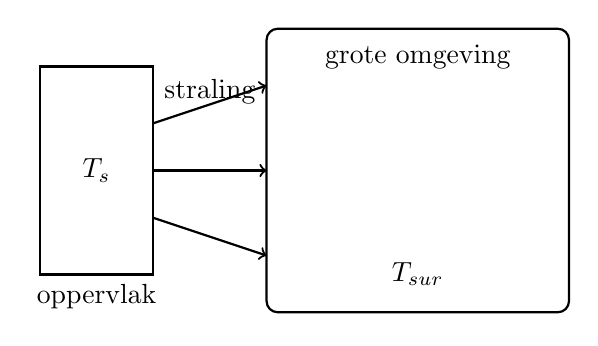
\begin{tikzpicture}[x=1.2cm,y=1.2cm]
        % hot surface
        \draw[thick] (0,0) rectangle (1.2,2.2);
        \node at (0.6,1.1) {$T_s$};
        \node[below] at (0.6,0) {oppervlak};

        % surroundings
        \draw[thick,rounded corners=4pt] (2.4,-0.4) rectangle (5.6,2.6);
        \node at (4.0,2.3) {grote omgeving};
        \node at (4.0,0.0) {$T_{sur}$};

        % radiation arrows
        \draw[thick,->] (1.2,1.6) -- (2.4,2.0);
        \draw[thick,->] (1.2,1.1) -- (2.4,1.1);
        \draw[thick,->] (1.2,0.6) -- (2.4,0.2);
        \node[above] at (1.8,1.7) {straling};
    \end{tikzpicture}
    \caption{Schematische stralingsuitwisseling tussen een oppervlak en een grote omgeving.}
\end{figure}

\part{Oefeningen Warmte en Stromingen}
\chapter{Oefeningen}
\section{Oefenzitting 1\&2: Hydrostatica}
\setcounter{opgave}{0}
\subsection*{Belangrijke Formules}
\begin{itemize}
    \item \textbf{Hydrostatische druk:} $P = P_{atm} + \rho g h$ \\
    Beschrijft de druk op een diepte $h$ in een stilstaande vloeistof.
    \item \textbf{Hydrostatische kracht op een vlak:} $F_R = P_{gem} A = (P_0 + \rho g h_c) A$ \\
    De totale kracht op een ondergedompeld oppervlak, werkend op het drukpunt.
    \item \textbf{Locatie drukpunt:} $y_p = y_c + \frac{I_{xx,c}}{y_c A}$ \\
    De verticale positie waar de resultante kracht aangrijpt met {$y_c$} het centerpunt ($y_p$ altijd dieper dan centerpunt $y_c$).
    \item \textbf{Oppervlakte en traagheidsmomenten:} \\
    Rechthoek: $A = b h$, $I_{xx,c} = \frac{b h^3}{12}$ (as door het zwaartepunt, evenwijdig met het vrije oppervlak). \\
    Cirkel: $A = \pi R^2$, $I_{xx,c} = \frac{\pi R^4}{4}$.
    \item \textbf{Netto druk (binnen/buiten):} $p_{net}(h) = (P_0 + \rho g h) - P_{in}$ \\
    Handig als binnenin een constante druk $P_{in}$ heerst (bv. lucht op $P_{atm}$).
    \item \textbf{Wet van Archimedes:} $F_b = \rho_{vloeistof} g V_{onder}$ \\
    De opwaartse kracht is gelijk aan het gewicht van de verplaatste vloeistof.
    \item \textbf{Drijvend object:} $F_b = W_{object} \Rightarrow \rho_{vloeistof} V_{onder} = \rho_{object} V_{totaal}$ \\
    Voor een object dat in evenwicht drijft.
    \item \textbf{Dichtheid via wegen in lucht en in water:} $\displaystyle \rho_{obj}=\rho_{vloeistof}\,\frac{W_{lucht}}{W_{lucht}-W_{in\,vloeistof}}$ \\
    Gebruikt Archimedes: $W_{lucht}-W_{in\,vloeistof}=F_b=\rho_{vloeistof}gV$.
    \item \textbf{Drukpunt op een schuine vlakke plaat:} $\displaystyle s_p = \bar{s} + \frac{I_{G}}{\bar{s}A}$ met $\bar{s}=\frac{h_c}{\sin\theta}$ \\
    $s$ is afstand langs de plaat gemeten vanaf het vrije oppervlak.
\end{itemize}

\begin{figure}[H]
    \centering
    \includegraphics[width=0.4\textwidth]{assets/hydrostatica.png}
    \caption{Hydrostatische krachten op een ondergedompeld vlak oppervlak.}
    \label{fig:hydrostatics}
\end{figure}


\opgave{Manometer en Drukverschil}
\textbf{Gegeven:}
Een manometer met kwik ($\rho_{Hg} = 13.600 \, kg/m^3$) is aangesloten op een tank met gas. Het niveauverschil in de manometer is $h = 40 \, cm$. De atmosferische druk is $P_{atm} = 101 \, kPa$. De zwaartekrachtversnelling is $g = 9,81 \, m/s^2$.

\textbf{Gevraagd:}
Bepaal de absolute druk in de tank.

\textbf{Oplossing:}
De druk in de tank duwt de kwikkolom omlaag. Op het scheidingsvlak (isobaar vlak) geldt dat de druk in de linker- en rechtertak gelijk moet zijn.
\[ P_{tank} = P_{atm} + \rho_{Hg} g h \]
Invullen van de waarden:
\[ P_{tank} = 101.000 \, Pa + (13.600 \, kg/m^3)(9,81 \, m/s^2)(0,40 \, m) \]
\[ P_{tank} = 101.000 + 53.366,4 \, Pa \]
\[ P_{tank} \approx 154,4 \, kPa \]

\opgave{Kracht op een Ondergedompeld Luik}
\textbf{Gegeven:}
Een rechthoekig luik van $2 \, m$ breed en $3 \, m$ hoog bevindt zich verticaal in een waterreservoir. De bovenkant van het luik bevindt zich $1 \, m$ onder het wateroppervlak.

\textbf{Gevraagd:}
De totale hydrostatische kracht op het luik en de locatie van het drukpunt.

\textbf{Oplossing:}
De gemiddelde druk werkt op het zwaartepunt (centroid) van het luik.
De diepte van het zwaartepunt $h_c$ is:
\[ h_c = 1 \, m + \frac{3 \, m}{2} = 2,5 \, m \]
De gemiddelde druk is:
\[ P_{gem} = \rho g h_c = 1000 \cdot 9,81 \cdot 2,5 = 24.525 \, Pa \]
De totale kracht is:
\[ F_R = P_{gem} \cdot A = 24.525 \cdot (2 \cdot 3) = 147.150 \, N \approx 147,2 \, kN \]
De locatie van het drukpunt $y_p$ (gemeten vanaf het oppervlak):
\[ y_p = y_c + \frac{I_{xx,c}}{y_c A} \]
Met $y_c = h_c = 2,5 \, m$ en $I_{xx,c} = \frac{b h^3}{12} = \frac{2 \cdot 3^3}{12} = 4,5 \, m^4$.
\[ y_p = 2,5 + \frac{4,5}{2,5 \cdot 6} = 2,5 + \frac{4,5}{15} = 2,5 + 0,3 = 2,8 \, m \]
Het drukpunt ligt dus $0,3 \, m$ onder het zwaartepunt.

\opgave{Vlakke schuine klep met parabolische vorm (kracht en druklijn)}
                    	\textbf{Gegeven:}
Een open bezinktank bevat een vloeistofsuspensie met dichtheid $\rho = 850\,\mathrm{kg/m^3}$. Een schuine klep maakt een hoek $\theta = 60^\circ$ met de horizontaal en is scharnierend aan de bodem. De vloeistofhoogte is $5\,\mathrm{m}$.

De vorm van de klep (in haar vlak) wordt beschreven door het gebied begrensd door $x=0$, $y=3\,\mathrm{m}$ en de parabool $y=2x^2$. De klep heeft een breedte (in de diepte) $b=2\,\mathrm{m}$.
\IfFileExists{assets/ex_11_20.png}{%
\begin{figure}[H]
    \centering
    \includegraphics[width=0.88\linewidth]{assets/ex_11_20.png}
    \caption{Opgavebeeld: schuine klep in bezinktank (indien aanwezig).}
\end{figure}
}{}

    \textbf{Gevraagd:}
Bepaal de resulterende hydrostatische kracht op de klep en de lijn van werking (afstand vanaf de onderkant langs de klep).

\IfFileExists{assets/ex_11_20_schema.png}{%
\begin{figure}[H]
    \centering
    \includegraphics[width=0.6\linewidth]{assets/ex_11_20_schema.png}
    \caption{Schematische voorstelling (vormdetails in de opgavefiguur).}
\end{figure}
}{%
\begin{figure}[H]
    \centering
    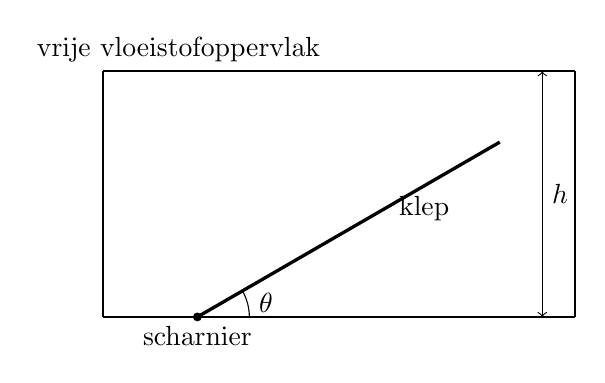
\begin{tikzpicture}[x=1.2cm,y=1.2cm]
        % water surface
        \draw[thick] (0,2.6) -- (5.0,2.6);
        \node[above] at (0.8,2.6) {vrije vloeistofoppervlak};

        % tank walls
        \draw[thick] (0,0) -- (0,2.6);
        \draw[thick] (5.0,0) -- (5.0,2.6);
        \draw[thick] (0,0) -- (5.0,0);

        % inclined gate
        \draw[very thick] (1.0,0) -- (4.2,1.85);
        \fill (1.0,0) circle (1.6pt);
        \node[below] at (1.0,0) {scharnier};
        \node at (3.4,1.15) {klep};

        % angle marker
        \draw (1.55,0) arc (0:30:0.55);
        \node[right] at (1.55,0.15) {$\theta$};

        % depth indicator
        \draw[thin,<->] (4.65,2.6) -- (4.65,0);
        \node[right] at (4.65,1.3) {$h$};
    \end{tikzpicture}
    \caption{Schematische voorstelling van de bezinktank met schuine klep.}
\end{figure}
}

    \textbf{Oplossing:}
We behandelen de klep als \emph{een vlak oppervlak} op een helling.

    \textbf{1) Oppervlakte van de parabolische vorm (in het vlak)}
Voor $y=3$ is $x=a=\sqrt{\frac{3}{2}}$.
De oppervlakte van het gebied begrensd door $x=0$, $y=3$ en $y=2x^2$ is gelijk aan:
\[
A_{vlak} = A_{rechthoek}-A_{parabool} = a\,h - \int_0^a 2x^2\,dx
        = a\cdot 3 - \frac{2}{3}a^3
\]
Met $a=\sqrt{\tfrac{3}{2}}$ volgt:
\[
A_{vlak} = 3\sqrt{\frac{3}{2}} - \frac{2}{3}\left(\sqrt{\frac{3}{2}}\right)^3 \approx 2{,}449\,\mathrm{m^2}
\]
De totale klepoppervlakte is $A=b\,A_{vlak}=2\cdot 2{,}449=4{,}898\,\mathrm{m^2}$.

    \textbf{2) Diepte van het zwaartepunt}
Voor dit parabolische gebied ligt het zwaartepunt op
\[
\bar{y} = \frac{3}{5}h = \frac{3}{5}\cdot 3 = 1{,}8\,\mathrm{m}
\]
gemeten vanaf de onderkant langs de klep.
De verticale diepte van het zwaartepunt onder het vrije oppervlak wordt dan:
\[
h_c = 5 - \bar{y}\sin\theta = 5 - 1{,}8\sin 60^\circ \approx 3{,}44\,\mathrm{m}
\]

    \textbf{3) Resultante kracht}
\[
F_R = \rho g h_c A = 850\cdot 9{,}81\cdot 3{,}44\cdot 4{,}898 \approx 1{,}40\times 10^5\,\mathrm{N} = 140\,\mathrm{kN}
\]

    \textbf{4) Lijn van werking (drukpunt) langs de klep}
We gebruiken de formule in afstanden langs de klep gemeten vanaf het vrije oppervlak.
De afstand van het vrije oppervlak tot het scharnier langs de klep is:
\[
L = \frac{5}{\sin 60^\circ} \approx 5{,}773\,\mathrm{m}
\]
Daarmee is de afstand van het vrije oppervlak tot het zwaartepunt:
\[
\bar{s} = L-\bar{y} = 5{,}773-1{,}8=3{,}973\,\mathrm{m}
\]
We hebben $I_G$ nodig t.o.v. de centroidale as evenwijdig met het vrije oppervlak.
Eerst het traagheidsmoment t.o.v. $y=0$ (in het vlak, per meter breedte):
\[
I_{x,0} = I_{rechthoek}-I_{parabool} = \frac{a h^3}{3} - \int_0^a \frac{(2x^2)^3}{3}\,dx
      = \frac{a\,3^3}{3} - \frac{8}{21}a^7 \approx 9{,}450\,\mathrm{m^4}
\]
Dan centroidaal (per meter breedte):
\[
I_{x,c} = I_{x,0} - A_{vlak}\,\bar{y}^2 = 9{,}450 - 2{,}449\cdot (1{,}8)^2 \approx 1{,}518\,\mathrm{m^4}
\]
Voor breedte $b=2$ wordt $I_G=bI_{x,c}=3{,}036\,\mathrm{m^4}$.
Nu:
\[
s_p = \bar{s} + \frac{I_G}{\bar{s}A} = 3{,}973 + \frac{3{,}036}{3{,}973\cdot 4{,}898} \approx 4{,}129\,\mathrm{m}
\]
Dus de lijn van werking ligt op afstand vanaf de onderkant (scharnier) langs de klep:
\[
y_p = L - s_p = 5{,}773-4{,}129=1{,}64\,\mathrm{m}
\]


\opgave{Hydrostatische Druk (Duikboot)}
\textbf{Gegeven:} Een duikboot bevindt zich op $175 \, ft$ ($53,34 \, m$) diepte in zee. De dichtheid van zeewater is $1025 \, kg/m^3$.

\textbf{Gevraagd:} De hydrostatische druk op de romp.

\textbf{Oplossing:}
\[ P = \rho g h = 1025 \, kg/m^3 \cdot 9,81 \, m/s^2 \cdot 53,34 \, m \]
\[ P = 536.345 \, Pa \approx 536 \, kPa \approx 5,36 \, bar \]

\opgave{Druk door Gewicht (Vrouw op Hakken)}
\textbf{Gegeven:} Een vrouw van $70 \, kg$ staat op de grond. De totale oppervlakte van haar schoenzolen is $400 \, cm^2$.

\textbf{Gevraagd:} De druk die zij uitoefent op de grond.

\textbf{Oplossing:}
De kracht is gelijk aan haar gewicht:
\[ F = m \cdot g = 70 \, kg \cdot 9,81 \, m/s^2 = 686,7 \, N \]
De oppervlakte in $m^2$:
\[ A = 400 \, cm^2 = 400 \cdot 10^{-4} \, m^2 = 0,04 \, m^2 \]
De druk is:
\[ P = \frac{F}{A} = \frac{686,7 \, N}{0,04 \, m^2} = 17.167,5 \, Pa \approx 17,2 \, kPa \]

\opgave{Drijvend IJsblok}
\textbf{Gegeven:}
Een ijsblok ($\rho_{ijs} = 917 \, kg/m^3$) drijft in zeewater ($\rho_{zee} = 1025 \, kg/m^3$).

\textbf{Gevraagd:}
Welk percentage van het volume van het ijsblok bevindt zich onder water?

\textbf{Oplossing:}
Volgens de wet van Archimedes is de opwaartse kracht gelijk aan het gewicht van de verplaatste vloeistof. Voor een drijvend object is de opwaartse kracht gelijk aan het eigen gewicht.
\[ F_{b} = W_{ijs} \]
\[ \rho_{zee} g V_{onder} = \rho_{ijs} g V_{totaal} \]
De verhouding is:
\[ \frac{V_{onder}}{V_{totaal}} = \frac{\rho_{ijs}}{\rho_{zee}} = \frac{917}{1025} \approx 0,895 \]
Dus $89,5\%$ van het ijsblok bevindt zich onder water.

\opgave{Archimedes en de kroon (dichtheid via wegen in lucht en water)}
          	\textbf{Gegeven:}
Een onregelmatig gevormde kroon weegt $3{,}55\,\mathrm{kgf}$ ($=34{,}8\,\mathrm{N}$) in lucht en $3{,}25\,\mathrm{kgf}$ ($=31{,}9\,\mathrm{N}$) in water. Neem $\rho_{water}=1000\,\mathrm{kg/m^3}$ en $g=9{,}81\,\mathrm{m/s^2}$. De dichtheid van goud is $\rho_{Au}=19\,300\,\mathrm{kg/m^3}$.
\IfFileExists{assets/ex_11_36.png}{%
\begin{figure}[H]
    \centering
    \includegraphics[width=0.88\linewidth]{assets/ex_11_36.png}
    \caption{Opgavebeeld: Archimedes en de kroon (indien aanwezig).}
\end{figure}
}{}

                    	\textbf{Gevraagd:}
Bepaal of de kroon uit puur goud bestaat. Bespreek ook hoe je dit kan doen met een gewone emmer zonder volumeverdeling.

\begin{figure}[H]
    \centering
    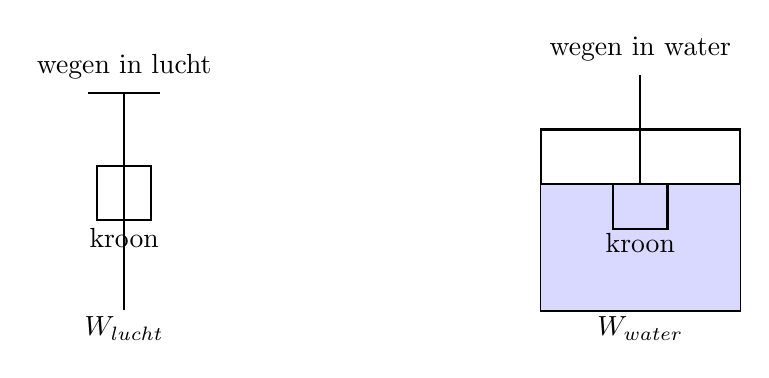
\begin{tikzpicture}[x=1.15cm,y=1.15cm]
        % left: in air
        \draw[thick] (0,0) -- (0,2.4);
        \draw[thick] (-0.4,2.4) -- (0.4,2.4);
        \draw[thick] (0,2.4) -- (0,1.6);
        \draw[thick] (-0.3,1.6) rectangle (0.3,1.0);
        \node at (0,0.8) {kroon};
        \node[above] at (0,2.45) {wegen in lucht};
        \node at (0,-0.2) {$W_{lucht}$};

        % right: in water
        \begin{scope}[shift={(4.6,0)}]
            \draw[thick] (0,0) rectangle (2.2,2.0);
            \fill[blue!15] (0,0) rectangle (2.2,1.4);
            \draw[thick] (0,1.4) -- (2.2,1.4);
            \draw[thick] (1.1,2.6) -- (1.1,1.4);
            \draw[thick] (0.8,1.4) rectangle (1.4,0.9);
            \node at (1.1,0.75) {kroon};
            \node[above] at (1.1,2.65) {wegen in water};
            \node at (1.1,-0.2) {$W_{water}$};
        \end{scope}
    \end{tikzpicture}
    \caption{Principe: verschil in gewicht geeft de opwaartse kracht.}
\end{figure}

                    	\textbf{Oplossing:}
Het verschil tussen beide gemeten gewichten is de opwaartse kracht:
\[
F_b = W_{lucht}-W_{water} = 34{,}8-31{,}9=2{,}9\,\mathrm{N}
\]
Volgens Archimedes geldt $F_b=\rho_{water}gV$, dus:
\[
V = \frac{F_b}{\rho_{water}g} = \frac{2{,}9}{1000\cdot 9{,}81} \approx 2{,}96\times 10^{-4}\,\mathrm{m^3}
\]
De massa volgt uit wegen in lucht ($W=mg$):
\[
m=\frac{W_{lucht}}{g}=\frac{34{,}8}{9{,}81}\approx 3{,}55\,\mathrm{kg}
\]
De gemiddelde dichtheid van de kroon is:
\[
\rho_{kroon} = \frac{m}{V} \approx \frac{3{,}55}{2{,}96\times 10^{-4}} \approx 1{,}20\times 10^4\,\mathrm{kg/m^3}
\]
Dit is duidelijk kleiner dan $\rho_{Au}=19\,300\,\mathrm{kg/m^3}$, dus de kroon is \textbf{niet} uit puur goud.

                    	\textbf{Zonder de kroon in water te wegen (emmer zonder schaal):}
Vul een emmer tot aan de rand met water. Dompel de kroon volledig onder (zonder de bodem te raken) en vang het overlopende water op. Weeg het overgelopen water in lucht: $m_{over}$.
Dan geldt $V = \frac{m_{over}}{\rho_{water}}$ en met $m=\frac{W_{lucht}}{g}$ kan je opnieuw $\rho_{kroon}=\frac{m}{V}$ bepalen.

    \opgave{Autoportier onder water (kracht en drukpunt)}
	\textbf{Gegeven:}
Een auto is ondergedompeld in een meer. Het bestuurdersportier is $h = 1{,}1\,\mathrm{m}$ hoog en $b = 0{,}9\,\mathrm{m}$ breed. De bovenrand van het portier bevindt zich op $10\,\mathrm{m}$ onder het wateroppervlak.
\IfFileExists{assets/ex_11_07.png}{%
\begin{figure}[H]
    \centering
    \includegraphics[width=0.88\linewidth]{assets/ex_11_07.png}
    \caption{Opgavebeeld: autoportier onder water (indien aanwezig).}
\end{figure}
}{}
\begin{enumerate}[label=(\alph*)]
    \item De auto is goed afgesloten en bevat binnenin lucht op atmosferische druk.
    \item De auto is volledig gevuld met water.
\end{enumerate}

                    	\textbf{Gevraagd:}
De netto kracht (loodrecht op het portier) en de locatie van het drukpunt.

\begin{figure}[H]
    \centering
    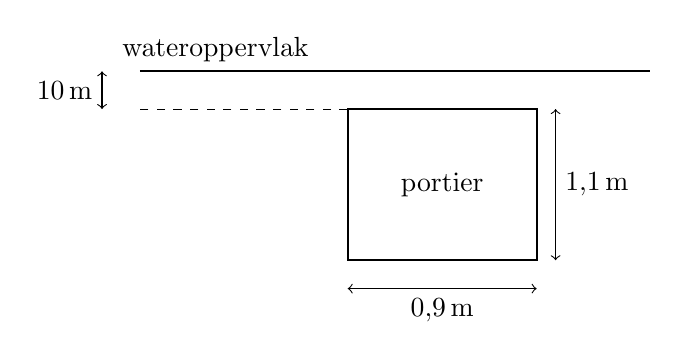
\begin{tikzpicture}[x=1.2cm,y=1.2cm]
        % water surface
        \draw[thick] (-0.2,2) -- (5.2,2);
        \node[above] at (0.6,2) {wateroppervlak};

        % door rectangle
        \draw[thick] (2,0.0) rectangle (4,1.6);
        \node at (3,0.8) {portier};

        % dimensions
        \draw[<->] (4.2,0.0) -- (4.2,1.6);
        \node[right] at (4.2,0.8) {$1{,}1\,\mathrm{m}$};
        \draw[<->] (2, -0.3) -- (4,-0.3);
        \node[below] at (3,-0.3) {$0{,}9\,\mathrm{m}$};

        % depth to top edge
        \draw[dashed] (2,1.6) -- (-0.2,1.6);
        \draw[<->] (-0.6,2) -- (-0.6,1.6);
        \node[left] at (-0.6,1.8) {$10\,\mathrm{m}$};
    \end{tikzpicture}
    \caption{Schematische voorstelling van het ondergedompelde portier.}
\end{figure}

	\textbf{Oplossing:}
	\textbf{(a) Binnenlucht op $P_{atm}$:}
De netto druk is gelijk aan de (buiten) hydrostatische overdruk: $p_{net}(h)=\rho g h$.
De diepte van het zwaartepunt is:
\[ h_c = 10 + \frac{1{,}1}{2} = 10{,}55\,\mathrm{m} \]
De oppervlakte is $A=b\,h=0{,}9\cdot 1{,}1=0{,}99\,\mathrm{m^2}$.
De resultante kracht:
\[
F = \rho g h_c A = 1000\cdot 9{,}81\cdot 10{,}55\cdot 0{,}99 \approx 1{,}025\times 10^5\,\mathrm{N} = 102{,}5\,\mathrm{kN}
\]
Het drukpunt (diepte onder het wateroppervlak):
\[
I_{xx,c}=\frac{b h^3}{12}=\frac{0{,}9\cdot (1{,}1)^3}{12}=0{,}0998\,\mathrm{m^4}
\]
\[
h_p = h_c + \frac{I_{xx,c}}{h_c A} = 10{,}55 + \frac{0{,}0998}{10{,}55\cdot 0{,}99} \approx 10{,}56\,\mathrm{m}
\]

	\textbf{(b) Auto gevuld met water:}
Aan beide zijden van het portier staat hetzelfde flu\"{i}dum (water) op dezelfde diepte, dus de drukverdeling is (bij benadering) identiek.
Daarom is de netto druk $p_{net}(h)\approx 0$ en dus:
\[ F \approx 0 \]
Een drukpunt is dan niet zinvol te defini\"eren.

\opgave{Ronde patrijspoort (kracht en drukpunt)}
	\textbf{Gegeven:}
Een ronde patrijspoort met diameter $D=0{,}30\,\mathrm{m}$ bevindt zich in de romp van een schip. Het midden van de patrijspoort ligt $h_c=4{,}0\,\mathrm{m}$ onder het wateroppervlak. Zeewater heeft soortelijke massa $\rho = 1{,}025\cdot 1000=1025\,\mathrm{kg/m^3}$.
\IfFileExists{assets/ex_11_10.png}{%
\begin{figure}[H]
    \centering
    \includegraphics[width=0.88\linewidth]{assets/ex_11_10.png}
    \caption{Opgavebeeld: ronde patrijspoort (indien aanwezig).}
\end{figure}
}{}

                    	\textbf{Gevraagd:}
De hydrostatische kracht op de patrijspoort en de diepte van het drukpunt.

\begin{figure}[H]
    \centering
    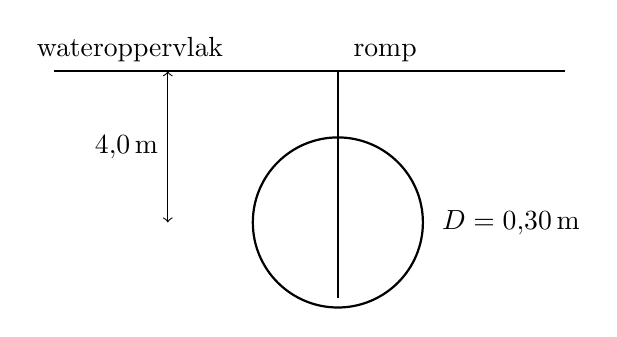
\begin{tikzpicture}[x=1.2cm,y=1.2cm]
        \draw[thick] (-0.2,2.2) -- (5.2,2.2);
        \node[above] at (0.6,2.2) {wateroppervlak};

        % hull line
        \draw[thick] (2.8,-0.2) -- (2.8,2.2);
        \node[above] at (3.3,2.2) {romp};

        % window circle
        \draw[thick] (2.8,0.6) circle (0.9);
        \node[right] at (3.8,0.6) {$D=0{,}30\,\mathrm{m}$};

        % depth to center
        \draw[<->] (1.0,2.2) -- (1.0,0.6);
        \node[left] at (1.0,1.4) {$4{,}0\,\mathrm{m}$};
    \end{tikzpicture}
    \caption{Schematische patrijspoort op diepte $h_c$.}
\end{figure}

	\textbf{Oplossing:}
Straal $R=D/2=0{,}15\,\mathrm{m}$.
\[ A=\pi R^2 = \pi (0{,}15)^2 = 0{,}0707\,\mathrm{m^2} \]
\[
F=\rho g h_c A = 1025\cdot 9{,}81\cdot 4{,}0\cdot 0{,}0707 \approx 2{,}84\times 10^3\,\mathrm{N} = 2{,}84\,\mathrm{kN}
\]
Voor het drukpunt gebruiken we $I_{xx,c}=\frac{\pi R^4}{4}$:
\[
I_{xx,c} = \frac{\pi (0{,}15)^4}{4} = 3{,}98\times 10^{-4}\,\mathrm{m^4}
\]
\[
h_p = h_c + \frac{I_{xx,c}}{h_c A} = 4{,}0 + \frac{3{,}98\times 10^{-4}}{4{,}0\cdot 0{,}0707} \approx 4{,}001\,\mathrm{m}
\]

\opgave{Cilindrische tank met overdruk (kracht op eindvlak)}
	\textbf{Gegeven:}
Een cilindrische tank is volledig gevuld met water. Op het vrije oppervlak wordt een extra druk $P_0$ aangelegd door een compressor. Het eindvlak is een cirkel met diameter $D=0{,}80\,\mathrm{m}$ (straal $R=0{,}40\,\mathrm{m}$). Neem $\rho=1000\,\mathrm{kg/m^3}$ en $g=9{,}81\,\mathrm{m/s^2}$. Beschouw drie gevallen: $P_0=0$, $P_0=3\,\mathrm{bar}$ en $P_0=10\,\mathrm{bar}$.
\IfFileExists{assets/ex_11_19.png}{%
\begin{figure}[H]
    \centering
    \includegraphics[width=0.88\linewidth]{assets/ex_11_19.png}
    \caption{Opgavebeeld: cilindrische tank met overdruk (indien aanwezig).}
\end{figure}
}{}

        \textbf{Gevraagd:}
De hydrostatische resultante op het eindvlak.

\begin{figure}[H]
    \centering
    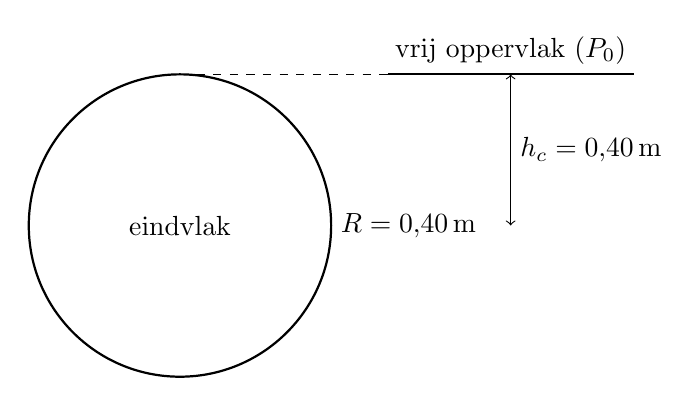
\begin{tikzpicture}[x=1.2cm,y=1.2cm]
        % end circle
        \draw[thick] (0,0) circle (1.6);
        \node at (0,0) {eindvlak};
        \node[right] at (1.6,0) {$R=0{,}40\,\mathrm{m}$};

        % water surface indicator at top
        \draw[thick] (2.2,1.6) -- (4.8,1.6);
        \node[above] at (3.5,1.6) {vrij oppervlak ($P_0$)};
        \draw[dashed] (0,1.6) -- (2.2,1.6);

        % centroid depth
        \draw[<->] (3.5,1.6) -- (3.5,0);
        \node[right] at (3.5,0.8) {$h_c=0{,}40\,\mathrm{m}$};
    \end{tikzpicture}
    \caption{Eindvlak met druk $P_0$ op het vrije oppervlak (schematisch).}
\end{figure}

	\textbf{Oplossing:}
Voor een vlak oppervlak geldt:
\[ F = (P_0 + \rho g h_c)A \]
Hier is $h_c=R=0{,}40\,\mathrm{m}$ en $A=\pi R^2=\pi(0{,}40)^2=0{,}503\,\mathrm{m^2}$.
De hydrostatische bijdrage door diepte is:
\[ \rho g h_c = 1000\cdot 9{,}81\cdot 0{,}40 = 3924\,\mathrm{Pa} \]
Daarmee:
\begin{itemize}
    \item $P_0=0$: $F = 3924\cdot 0{,}503 \approx 1{,}97\times 10^3\,\mathrm{N}$.
    \item $P_0=3\,\mathrm{bar}=300\,\mathrm{kPa}$: $F=(300000+3924)\cdot 0{,}503 \approx 1{,}53\times 10^5\,\mathrm{N}=153\,\mathrm{kN}$.
    \item $P_0=10\,\mathrm{bar}=1{,}0\,\mathrm{MPa}$: $F=(1000000+3924)\cdot 0{,}503 \approx 5{,}05\times 10^5\,\mathrm{N}=505\,\mathrm{kN}$.
\end{itemize}


\section{Oefenzitting 3: Stromingsleer\&Bernoulli en energievergelijking}
\setcounter{opgave}{0}
\subsection*{Belangrijke Formules}
\begin{itemize}
    \item \textbf{Bernoulli-vergelijking:} $P + \frac{1}{2}\rho V^2 + \rho g z = \text{constant}$ \\
    Geldt langs een stroomlijn voor stationaire, onsamendrukbare en wrijvingsloze stroming.
    \item \textbf{Continuïteitsvergelijking:} $A_1 V_1 = A_2 V_2$ \\
    Behoud van massa voor onsamendrukbare stroming in een buis.
    \item \textbf{Pitot-statisch:} $\Delta p = p_0-p = \frac{1}{2}\rho V^2 \Rightarrow V=\sqrt{\frac{2\Delta p}{\rho}}$ \\
    Relatie tussen snelheidsdruk en snelheid.
    \item \textbf{Drukverschil via manometer (Hg):} $\Delta p = (\rho_{Hg}-\rho)g\,\Delta h$ \\
    Voor een differentiaalmanometer met kwik op een waterleiding.
    \item \textbf{Debiet uit tank/orifice (zonder verliezen):} $V = \sqrt{2\left(\frac{\Delta p}{\rho}+g\Delta z\right)}$, $Q=AV$ \\
    Met $\Delta p=p_{boven}-p_{uit}$ en $\Delta z=z_{boven}-z_{uit}$.
    \item \textbf{Netto vermogen uit turbine (controlevolume):} $\dot{W}_{as} = \eta\,\dot{m}\left(\frac{\Delta p}{\rho}+\frac{V_1^2-V_2^2}{2}+g(z_1-z_2)\right)$ \\
    Zonder warmteoverdracht en verliezen; $\eta$ is turbine-generator efficiëntie.
    \item \textbf{Impulsvergelijking (lineair):} $\sum \vec{F} = \dot{m} (\vec{V}_{uit} - \vec{V}_{in})$ \\
    De som van externe krachten op een controlevolume is gelijk aan de verandering in impulsstroom.
    \item \textbf{Massadebiet:} $\dot{m} = \rho A V$ \\
    De hoeveelheid massa die per tijdseenheid door een doorsnede stroomt.
\end{itemize}


\opgave{Pitot-statisch meetsonde (vliegtuigsnelheid)}
	\textbf{Gegeven:}
Een pitot-statische sonde meet de snelheid van een vliegtuig op $3000\,\mathrm{m}$ hoogte. Het gemeten differentiaaldrukverschil is $\Delta p=3\,\mathrm{kPa}$. De luchtdichtheid is $\rho_{lucht}=0{,}909\,\mathrm{kg/m^3}$.
\IfFileExists{assets/ex_12_15.png}{%
\begin{figure}[H]
    \centering
    \includegraphics[width=0.88\linewidth]{assets/ex_12_15.png}
    \caption{Opgavebeeld: pitot-statisch (indien aanwezig).}
\end{figure}
}{}

	\textbf{Gevraagd:}
Bepaal de snelheid van het vliegtuig.

	\textbf{Oplossing:}
Voor een pitot-statisch systeem (incompressibel benadering) geldt:
\[
\Delta p = \frac{1}{2}\rho V^2
\]
Dus:
\[
V = \sqrt{\frac{2\Delta p}{\rho}} = \sqrt{\frac{2\cdot 3000}{0{,}909}} \approx \sqrt{6601} \approx 81{,}2\,\mathrm{m/s}
\]

\opgave{Tank met overdruk en uitlaat-orifice (debiet)}
	\textbf{Gegeven:}
Een drukvat met water heeft een opening onderaan met diameter $D=10\,\mathrm{cm}$ waar water naar de atmosfeer uitstroomt. Het waterniveau ligt $\Delta z = 2{,}5\,\mathrm{m}$ boven de uitlaat. De luchtdruk boven het water is $p_1=250\,\mathrm{kPa}$ (absoluut) en de atmosferische druk is $p_2=100\,\mathrm{kPa}$. Verwaarloos wrijvingsverliezen. Neem $\rho=1000\,\mathrm{kg/m^3}$ en $g=9{,}81\,\mathrm{m/s^2}$.
\IfFileExists{assets/ex_12_25.png}{%
\begin{figure}[H]   
    \centering
    \includegraphics[width=0.88\linewidth]{assets/ex_12_25.png}
    \caption{Opgavebeeld: tank met overdruk en uitlaat-orifice (indien aanwezig).}
\end{figure}
}{}

	\textbf{Gevraagd:}
Bepaal het initiële volumetrisch debiet $Q$.

	\textbf{Oplossing:}
We passen Bernoulli toe tussen het vrije oppervlak (1) en de uitlaat (2). Omdat het vat groot is nemen we $V_1\approx 0$.
\[
\frac{p_1}{\rho} + g z_1 = \frac{p_2}{\rho} + g z_2 + \frac{V_2^2}{2}
\]
Dus:
\[
\frac{V_2^2}{2} = \frac{p_1-p_2}{\rho} + g(z_1-z_2)
\]
Met $p_1-p_2 = 150\,\mathrm{kPa}=150000\,\mathrm{Pa}$ en $z_1-z_2=2{,}5\,\mathrm{m}$:
\[
V_2 = \sqrt{2\left(\frac{150000}{1000}+9{,}81\cdot 2{,}5\right)} = \sqrt{2(150+24{,}525)}\approx 18{,}7\,\mathrm{m/s}
\]
De orifice-oppervlakte:
\[
A = \frac{\pi D^2}{4} = \frac{\pi (0{,}10)^2}{4} = 7{,}854\times 10^{-3}\,\mathrm{m^2}
\]
Het debiet is $Q=AV$:
\[
Q = 7{,}854\times 10^{-3}\cdot 18{,}7 \approx 0{,}147\,\mathrm{m^3/s}
\]

\opgave{Maximale straalhoogte bij overdruk in tank}
	\textbf{Gegeven:}
Het waterniveau in een tank ligt $15\,\mathrm{m}$ boven de grond. Onderaan is een slang aangesloten en de nozzle aan het uiteinde wijst verticaal omhoog. Het deksel is luchtdicht en de luchtdruk boven het wateroppervlak is $3\,\mathrm{atm}$ \emph{gage}. Het systeem bevindt zich op zeeniveau. Verwaarloos verliezen. Neem $\rho=1000\,\mathrm{kg/m^3}$ en $g=9{,}81\,\mathrm{m/s^2}$.

\IfFileExists{assets/ex_12_34.png}{%
\begin{figure}[H]
    \centering
    \includegraphics[width=0.3\linewidth]{assets/ex_12_34.png}
    \caption{Opgavebeeld: drukvat met orifice (12-34) (indien aanwezig).}
\end{figure}
}{}
	\textbf{Gevraagd:}
Bepaal de maximale hoogte $h$ die de waterstraal kan bereiken.

	\textbf{Oplossing:}
We vergelijken het vrije oppervlak in de tank (1) met het hoogste punt van de straal (2). In punt (2) geldt $V_2=0$ en $p_2=p_{atm}$.

De tankdruk is $p_1=p_{atm}+3\,\mathrm{atm}$, dus $p_1-p_2=3\,\mathrm{atm}$.
Bernoulli zonder verliezen (met $V_1\approx 0$):
\[
\frac{p_1-p_2}{\rho g} + (z_1-z_2) = 0
\]
Als we $z_2$ kiezen als de maximale straalhoogte boven de nozzle, dan is $z_1-z_{nozzle}=15\,\mathrm{m}$.
De extra drukhoogte is:
\[
\frac{p_1-p_2}{\rho g} = \frac{3\cdot 101325}{1000\cdot 9{,}81} \approx 31{,}0\,\mathrm{m}
\]
Dus de maximale straalhoogte is:
\[
h = 15 + 31{,}0 \approx 46{,}0\,\mathrm{m}
\]

\opgave{Hydraulische turbine (vermogen uit drukval)}
	\textbf{Gegeven:}
Water stroomt een hydraulische turbine binnen via een buis met diameter $D_1=30\,\mathrm{cm}$ met debiet $Q=0{,}6\,\mathrm{m^3/s}$ en verlaat de turbine via een buis met diameter $D_2=25\,\mathrm{cm}$. De drukval over de turbine wordt gemeten met een kwikmanometer: $\Delta h = 1{,}2\,\mathrm{m\,Hg}$. De gecombineerde turbine-generator efficiëntie is $\eta=0{,}83$. Verwaarloos kinetische-energiecorrectiefactoren en hoogteverschil.
\IfFileExists{assets/ex_12_54.png}{%
\begin{figure}[H]
    \centering
    \includegraphics[width=0.88\linewidth]{assets/ex_12_54.png}
    \caption{Opgavebeeld: turbine met generator (indien aanwezig).}
\end{figure}
}{}

	\textbf{Gevraagd:}
Bepaal het netto elektrisch vermogen $\dot{W}_e$.

	\textbf{Oplossing:}
	\textbf{1) Snelheden uit continuïteit}
\[
A_1=\frac{\pi D_1^2}{4}=\frac{\pi (0{,}30)^2}{4}=0{,}0707\,\mathrm{m^2},\qquad V_1=\frac{Q}{A_1}=\frac{0{,}6}{0{,}0707}=8{,}49\,\mathrm{m/s}
\]
\[
A_2=\frac{\pi D_2^2}{4}=\frac{\pi (0{,}25)^2}{4}=0{,}0491\,\mathrm{m^2},\qquad V_2=\frac{Q}{A_2}=\frac{0{,}6}{0{,}0491}=12{,}2\,\mathrm{m/s}
\]

	\textbf{2) Drukval uit manometer}
Voor een differentiaalmanometer met kwik op een waterleiding nemen we:
\[
\Delta p=(\rho_{Hg}-\rho)g\Delta h
\]
Met $\rho_{Hg}=13600\,\mathrm{kg/m^3}$, $\rho=1000\,\mathrm{kg/m^3}$ en $\Delta h=1{,}2\,\mathrm{m}$:
\[
\Delta p=(13600-1000)\cdot 9{,}81\cdot 1{,}2 \approx 1{,}48\times 10^5\,\mathrm{Pa}
\]

	\textbf{3) Specifieke energiedaling en vermogen}
De specifieke energiedaling beschikbaar voor asvermogen (zonder $\Delta z$) is:
\[
e = \frac{\Delta p}{\rho}+\frac{V_1^2-V_2^2}{2}
\]
\[
\frac{\Delta p}{\rho}=\frac{1{,}48\times 10^5}{1000}=148\,\mathrm{m^2/s^2},\qquad \frac{V_1^2-V_2^2}{2}=\frac{(8{,}49)^2-(12{,}2)^2}{2}\approx -38{,}7\,\mathrm{m^2/s^2}
\]
\[
e\approx 148-38{,}7=109\,\mathrm{m^2/s^2}
\]
Het massadebiet is $\dot{m}=\rho Q=1000\cdot 0{,}6=600\,\mathrm{kg/s}$.
Het elektrisch vermogen (met efficiëntie) wordt:
\[
\dot{W}_e=\eta\,\dot{m}\,e=0{,}83\cdot 600\cdot 109 \approx 5{,}46\times 10^4\,\mathrm{W}=54{,}6\,\mathrm{kW}
\]




\section{Oefenzitting 4: Tabellen en eenheden}
\setcounter{opgave}{0}
\subsection*{Belangrijke Formules}
\begin{itemize}
    \item \textbf{Dichtheid:} $\rho = \frac{m}{V}$ \\
    Massa per volume-eenheid.
    \item \textbf{Tweede wet van Newton:} $F = m a$ \\
    Kracht is massa maal versnelling.
    \item \textbf{Gewicht:} $W = m g$ \\
    De zwaartekracht op een massa.
\end{itemize}


\section{Oefenzitting 5: Gesloten systemen}
\setcounter{opgave}{0}
\subsection*{Belangrijke Formules}
\begin{itemize}
    \item \textbf{Eerste Hoofdwet:} $Q - W = \Delta U$ \\
    Energiebehoud voor een gesloten systeem (geen massa-overdracht).
    \item \textbf{Grensverplaatsingsarbeid:} $W_b = \int P dV$ \\
    Arbeid geleverd door expansie of compressie.
    \item \textbf{Isobaar proces:} $W_b = P(V_2 - V_1)$ \\
    Arbeid bij constante druk.
\end{itemize}

\opgave{Zuiger-Cilinder}
\textbf{Gegeven:}
Gas expandeert isobaar ($P=200 \, kPa$) van $V_1 = 0,1 \, m^3$ naar $V_2 = 0,3 \, m^3$. Er wordt $50 \, kJ$ warmte toegevoerd.

\textbf{Gevraagd:}
De verandering in interne energie $\Delta U$.

\textbf{Oplossing:}
Arbeid $W_b = P(V_2 - V_1) = 200 (0,3 - 0,1) = 40 \, kJ$.
Eerste wet: $Q - W = \Delta U$.
$50 \, kJ - 40 \, kJ = \Delta U$.
$\Delta U = 10 \, kJ$.

\section{Oefenzitting 6: Open systemen}
\setcounter{opgave}{0}
\subsection*{Belangrijke Formules}
\begin{itemize}
    \item \textbf{Eerste Hoofdwet (Stationair):} $\dot{Q} - \dot{W} = \dot{m} \Delta (h + \frac{V^2}{2} + gz)$ \\
    Energiebehoud voor een open systeem (controlevolume) in stationaire toestand.
    \item \textbf{Enthalpie:} $h = u + Pv$ \\
    Combinatie van interne energie en stromingsarbeid.
    \item \textbf{Ideaal gas:} $\Delta h = c_p \Delta T$ \\
    Enthalpieverandering voor een ideaal gas met constante soortelijke warmte.

    Bekijk je tabellen voor specifieke waarden van $c_p$, $h$, T, $P$. Zorg dat je ziet wanneer je superheated, gesatureerd of vloeibaar hebt.
\end{itemize}

\opgave{Compressor (Helium)}
\begin{figure}[H]
    \centering
    \includegraphics[width=0.4\textwidth]{assets/compressor_exercise.png}
    \caption{Compressor met in- en uitgaande stromen.}
\end{figure}
\textbf{Gegeven:}
Helium wordt gecomprimeerd van $P_1 = 105 \, kPa$ en $T_1 = 295 \, K$ naar $P_2 = 700 \, kPa$ en $T_2 = 460 \, K$.
Er treedt een warmteverlies op van $q_{uit} = 15 \, kJ/kg$.
Het massadebiet is $\dot{m} = 60 \, kg/min$.
Kinetische energieveranderingen worden verwaarloosd.

\textbf{Gevraagd:}
Het benodigde vermogen $\dot{W}_{in}$.

\textbf{Oplossing:}
Voor een open systeem (compressor) geldt de eerste hoofdwet. Omdat Helium een ideaal gas is, geldt $\Delta h = c_p \Delta T$.
De energiebalans per eenheid massa (waarbij $w_{in}$ positief is voor toevoer en $q_{uit}$ positief voor verlies):
\[ w_{in} = \Delta h + q_{uit} = c_p(T_2 - T_1) + q_{uit} \]
Voor Helium is de soortelijke warmte bij constante druk $c_p = 5,1926 \, kJ/kgK$.
\[ w_{in} = 5,1926 \cdot (460 - 295) + 15 \]
\[ w_{in} = 5,1926 \cdot 165 + 15 = 856,78 + 15 = 871,8 \, kJ/kg \]
Het totale vermogen is:
\[ \dot{W}_{in} = \dot{m} \cdot w_{in} \]
Eerst het massadebiet omrekenen naar $kg/s$:
\[ \dot{m} = 60 \, kg/min = \frac{60}{60} \, kg/s = 1 \, kg/s \]
\[ \dot{W}_{in} = 1 \, kg/s \cdot 871,8 \, kJ/kg = 871,8 \, kW \]

\section{Oefenzitting 7: Eerste hoofdwet cycli}
\setcounter{opgave}{0}
\opgave{Stoomturbine}
\begin{figure}[H]
    \centering
    \includegraphics[width=0.4\textwidth]{assets/Turbine_oefening.png}
    \caption{Stoomturbine met in- en uitgaande stromen.}
\end{figure}
\textbf{Gegeven:}
Stoom stroomt door een turbine met een massadebiet $\dot{m} = 26 \, kg/s$.
Inlaat (1): $P_1 = 6 \, MPa$, $T_1 = 600^\circ C$, $V_1 \approx 0 \, m/s$.
Uitlaat (2): $P_2 = 0,5 \, MPa$, $T_2 = 200^\circ C$, $V_2 = 180 \, m/s$.
De turbine levert een vermogen van $\dot{W}_{out} = 20 \, MW$.
Hoogteverschillen zijn verwaarloosbaar ($\Delta z \approx 0$).

\textbf{Gevraagd:}
De warmteoverdracht $\dot{Q}_{uit}$ (warmteverlies).

\textbf{Oplossing:}
Uit superheated gas tabellen (of gegeven):
$h_1 = 3658,8 \, kJ/kg$
$h_2 = 2855,8 \, kJ/kg$
De verandering in kinetische energie:
\[ \Delta ke = \frac{V_2^2 - V_1^2}{2} = \frac{180^2 - 0}{2} = 16.200 \, J/kg = 16,2 \, kJ/kg \]
De energiebalans voor een open systeem (turbine):
\[ \dot{E}_{in} = \dot{E}_{out} \]
\[ \dot{m}(h_1 + \frac{V_1^2}{2}) = \dot{W}_{out} + \dot{Q}_{uit} + \dot{m}(h_2 + \frac{V_2^2}{2}) \]
Omschrijven voor $\dot{Q}_{uit}$:
\[ \dot{Q}_{uit} = \dot{m}(h_1 - h_2 - \frac{V_2^2}{2}) - \dot{W}_{out} \]
Invullen van de waarden (let op eenheden, $20 \, MW = 20.000 \, kW$):
\[ \dot{Q}_{uit} = 26 \left( 3658,8 - 2855,8 - 16,2 \right) - 20.000 \]
\[ \dot{Q}_{uit} = 26 \left( 786,8 \right) - 20.000 \]
\[ \dot{Q}_{uit} = 20.456,8 - 20.000 = 456,8 \, kW \]

\opgave{Expansieventiel (Koelmiddel-134a)}
\textbf{Gegeven:}
Koelmiddel-134a wordt gewurgd (throttled) van een verzadigde vloeistoftoestand bij $700 \, kPa$ naar een druk van $160 \, kPa$.

\textbf{Gevraagd:}
De temperatuurdaling $\Delta T$ en het uiteindelijke specifieke volume $v_2$.

\textbf{Oplossing:}
Voor een wurgproces (adiabatisch, geen arbeid, verwaarloosbare kinetische/potentiële energie) geldt dat de enthalpie constant blijft: $h_1 = h_2$.

\textit{Toestand 1:} $P_1 = 700 \, kPa$, verzadigde vloeistof ($x_1=0$).
Uit tabellen voor R-134a:
\[ T_1 = T_{sat@700kPa} = 26,69^\circ C \]
\[ h_1 = h_{f@700kPa} = 88,2 \, kJ/kg \]

\textit{Toestand 2:} $P_2 = 160 \, kPa$.
\[ h_2 = h_1 = 88,2 \, kJ/kg \]
Uit tabellen bij $160 \, kPa$:
\[ T_2 = T_{sat@160kPa} = -15,6^\circ C \]
\[ h_f = 31,21 \, kJ/kg, \quad h_g = 241,11 \, kJ/kg \]
Kwaliteit $x_2$ berekenen:
\[ h_2 = h_f + x_2 (h_g - h_f) \]
\[ 88,2 = 31,21 + x_2 (241,11 - 31,21) \]
\[ x_2 = \frac{88,2 - 31,21}{209,9} \approx 0,27 \]
Specifiek volume $v_2$ (met $v_g$ bij $160 \, kPa$):
\[v_2 = v_f + x_2 (v_g - v_f) \]
(je mag Vf verwaarlozen omdat het zo klein is vergeleken met Vg)
\[ v_2 \approx x_2 v_g \approx 0,0335 \, m^3/kg \]

Temperatuurdaling:
\[ \Delta T = T_1 - T_2 = 26,69 - (-15,6) = 42,3^\circ C \]

\section{Oefenzitting 8 : Entropie en tweede hoofdwet}
\setcounter{opgave}{0}
\subsection*{Belangrijke Formules}
\begin{itemize}
    \item \textbf{Thermisch rendement:} $\eta_{th} = \frac{W_{netto}}{Q_{in}} = 1 - \frac{Q_{uit}}{Q_{in}}$ \\
    Efficiëntie van een warmtemotor.
    \item \textbf{COP Warmtepomp:} $COP_{HP} = \frac{Q_H}{W_{in}}$ \\
    Prestatiecoëfficiënt voor verwarming.
    \item \textbf{COP Koelmachine:} $COP_{R} = \frac{Q_L}{W_{in}}$ \\
    Prestatiecoëfficiënt voor koeling.
\end{itemize}

\opgave{Warmtepomp}
\textbf{Gegeven:}
Een warmtepomp levert $10 \, kW$ warmte aan een huis ($20^\circ C$) en onttrekt warmte aan de buitenlucht ($0^\circ C$). De COP is $3,5$.

\textbf{Gevraagd:}
Het benodigde elektrische vermogen.

\textbf{Oplossing:}
$COP_{HP} = \frac{\dot{Q}_H}{\dot{W}_{in}}$.
$3,5 = \frac{10 \, kW}{\dot{W}_{in}}$.
$\dot{W}_{in} = \frac{10}{3,5} \approx 2,86 \, kW$.


\section{Oefenzitting 11: Navier-Stokes, Moody diagram, stromingsweerstand}
\setcounter{opgave}{0}
\subsection*{Belangrijke Formules}
\begin{itemize}
    \item \textbf{Reynoldsgetal:} $Re = \frac{\rho V D}{\mu} = \frac{V D}{\nu}$ \\
    Bepaalt of een stroming laminair ($Re < 2300$) of turbulent ($Re > 4000$) is.
    \item \textbf{Drukverlies (Darcy-Weisbach):} $\Delta P_L = f \frac{L}{D} \frac{\rho V^2}{2}$ \\
    Berekent het drukverlies door wrijving in een buis.
    \item \textbf{Wrijvingsfactor (Laminair):} $f = \frac{64}{Re}$ \\
    Geldt voor volledig ontwikkelde laminaire stroming in een ronde buis.
\end{itemize}

\opgave{Drukverlies in een Buis}
\textbf{Gegeven:}
Olie ($\rho = 900 \, kg/m^3, \nu = 10^{-4} \, m^2/s$) stroomt door een buis ($D=0,1 \, m, L=100 \, m$) met $V=2 \, m/s$.

\textbf{Gevraagd:}
Het drukverlies $\Delta P$.

\textbf{Oplossing:}
Reynoldsgetal: $Re = \frac{V D}{\nu} = \frac{2 \cdot 0,1}{10^{-4}} = 2000$.
Dit is laminair ($Re \le 2300$).
Wrijvingsfactor $f = \frac{64}{Re} = \frac{64}{2000} = 0,032$.
Drukverlies (Darcy-Weisbach):
\[ \Delta P = f \frac{L}{D} \frac{1}{2}\rho V^2 \]
\[ \Delta P = 0,032 \cdot \frac{100}{0,1} \cdot \frac{1}{2} \cdot 900 \cdot 2^2 \]
\[ \Delta P = 0,032 \cdot 1000 \cdot 1800 = 57.600 \, Pa = 57,6 \, kPa \]

\section{Oefenzitting 12: Turbulentie, leidingen, uitwendige stroming, drag\&lift force}
\setcounter{opgave}{0}
\opgave{Olievat (leidingverlies)}
\begin{figure}[H]
    \centering
    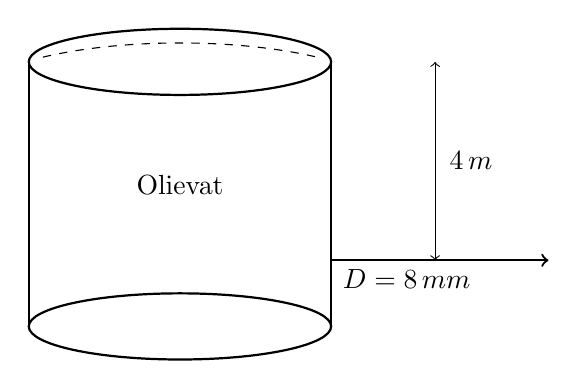
\begin{tikzpicture}[x=1.2cm,y=1.2cm]
        % Tank
        \draw[thick] (0,0) ellipse (1.6 and 0.35);
        \draw[thick] (-1.6,0) -- (-1.6,-2.8);
        \draw[thick] (1.6,0) -- (1.6,-2.8);
        \draw[thick] (0,-2.8) ellipse (1.6 and 0.35);
        % Vloeistofniveau (stippellijn)
        \draw[dashed] (-1.45,0.05) .. controls (-0.6,0.25) and (0.6,0.25) .. (1.45,0.05);
        % Leiding
        \draw[thick] (1.6,-2.1) -- (3.4,-2.1);
        \draw[thick,->] (3.4,-2.1) -- (3.9,-2.1);
        % Hoogtemaat 4 m
        \draw[thin,<->] (2.7,0.0) -- (2.7,-2.1);
        \node[right] at (2.75,-1.05) {$4\,m$};
        % Diameter label
        \node[below] at (2.4,-2.1) {$D=8\,mm$};
        % Labels
        \node at (0,-1.3) {Olievat};
    \end{tikzpicture}
    \caption{Olievat: afstroming uit een olievat via een lange dunne leiding.}
\end{figure}

                	\textbf{Gegeven:}
Olie met dichtheid $\rho = 850\,\mathrm{kg/m^3}$ en kinematische viscositeit $\nu = 0{,}00062\,\mathrm{m^2/s}$ stroomt uit een opslagtank (open naar de atmosfeer) via een horizontale buis met diameter $D=8\,\mathrm{mm}$ en lengte $L=40\,\mathrm{m}$. Het vloeistofniveau in de tank ligt $\Delta z = 4\,\mathrm{m}$ boven het buiscentrum. Kleine verliezen worden verwaarloosd.

                	\textbf{Gevraagd:}
Het volumetrisch debiet $Q$ door de leiding.

                	\textbf{Oplossing:}
We passen Bernoulli toe tussen het vrije vloeistofoppervlak (1) en de leiding-uitlaat (2).
Omdat de tank open is geldt $p_1=p_2=p_{atm}$ en omdat de tank groot is nemen we $V_1\approx 0$.
Met enkel leidingverlies (Darcy-Weisbach) volgt:
\[
\Delta z = \frac{V^2}{2g} + h_f,\qquad h_f = f\frac{L}{D}\frac{V^2}{2g}
\]
Dus:
\[
\Delta z = \left(1+ f\frac{L}{D}\right)\frac{V^2}{2g}
\]

Omdat $\nu$ zeer groot is, controleren we of de stroming laminair is. Voor laminaire stroming geldt:
\[
f = \frac{64}{Re},\qquad Re = \frac{VD}{\nu}
\]
Invullen van $f$ in $h_f$:
\[
h_f = \frac{64}{Re}\frac{L}{D}\frac{V^2}{2g}
= \frac{64\nu}{VD}\frac{L}{D}\frac{V^2}{2g}
= \frac{64\nu L}{D^2}\,\frac{V}{2g}
\]
De energievergelijking wordt dan lineair-kwadratisch in $V$:
\[
\Delta z = \frac{V^2}{2g} + \frac{64\nu L}{D^2}\,\frac{V}{2g}
\]
Vermenigvuldig met $2g$:
\[
2g\Delta z = V^2 + \left(\frac{64\nu L}{D^2}\right)V
\]
Met $g=9{,}81\,\mathrm{m/s^2}$, $\Delta z=4\,\mathrm{m}$, $\nu=0{,}00062\,\mathrm{m^2/s}$, $L=40\,\mathrm{m}$ en $D=0{,}008\,\mathrm{m}$:
\[
\frac{64\nu L}{D^2} = \frac{64\cdot 0{,}00062\cdot 40}{0{,}008^2} = 24800\,\mathrm{s^{-1}}
\]
Dus:
\[
78{,}48 = V^2 + 24800\,V
\]
Oplossen van de kwadratische vergelijking (positieve wortel):
\[
V = \frac{-24800 + \sqrt{24800^2 + 4\cdot 78{,}48}}{2} \approx 0{,}00316\,\mathrm{m/s}
\]
Reynoldsgetal:
\[
Re = \frac{VD}{\nu} = \frac{0{,}00316\cdot 0{,}008}{0{,}00062} \approx 0{,}041\ (<2300)\Rightarrow\ \text{laminair (aanname klopt).}
\]
Het debiet is $Q = AV$ met $A = \frac{\pi D^2}{4}$:
\[
A = \frac{\pi\,(0{,}008)^2}{4} = 5{,}03\times 10^{-5}\,\mathrm{m^2}
\]
\[
Q = AV = 5{,}03\times 10^{-5}\cdot 0{,}00316 \approx 1{,}59\times 10^{-7}\,\mathrm{m^3/s}
\]
Of in liter per seconde:
\[
Q \approx 1{,}59\times 10^{-4}\,\mathrm{L/s}\ (\approx 0{,}159\,\mathrm{mL/s})
\]

\opgave{Dimensieanalyse (Weerstandskracht)}
\textbf{Gegeven:}
De weerstandskracht $F_D$ hangt af van snelheid $V$, diameter $D$, dichtheid $\rho$ en viscositeit $\mu$.

\textbf{Gevraagd:}
Leid de dimensieloze groepen af met Buckingham Pi.

\textbf{Oplossing:}
Variabelen: $F_D, V, D, \rho, \mu$ ($n=5$).
Basisdimensies: $M, L, T$ ($j=3$).
Aantal Pi-groepen: $k = 5 - 3 = 2$.
Kies herhalende variabelen: $\rho, V, D$.
$\Pi_1 = F_D \rho^a V^b D^c \Rightarrow \frac{F_D}{\rho V^2 D^2} = C_D$ (Weerstandscoëfficiënt).
$\Pi_2 = \mu \rho^a V^b D^c \Rightarrow \frac{\mu}{\rho V D} = Re^{-1}$ (Reynoldsgetal).
Functioneel verband: $C_D = f(Re)$.

\chapter*{Conclusie}
Dit document heeft de kernprincipes van warmte en stroming samengevat. Van de fundamentele wetten van thermodynamica die energiebehoud dicteren, tot de complexe bewegingsvergelijkingen van fluïda. Het correct toepassen van deze principes vereist inzicht in de aannames (zoals incompressibiliteit of reversibiliteit) en nauwkeurigheid in berekeningen. Met de aangereikte theorie en oefeningen bent u toegerust om thermische en fluïdumtechnische systemen te analyseren.

\chapter*{Bijlagen}
\section*{Tabel 1: Samenvatting Dimensieloze Getallen}
\begin{table}[h]
\centering
\begin{tabular}{@{}llll@{}}
\toprule
\textbf{Getal} & \textbf{Symbool} & \textbf{Definitie} & \textbf{Fysische Betekenis} \\ \midrule
Reynolds & $Re$ & $\frac{\rho V L}{\mu}$ & Traagheidskrachten / Viskeuze krachten (Laminair vs Turbulent) \\
Prandtl & $Pr$ & $\frac{\nu}{\alpha}$ & Impulsdiffusie / Warmtediffusie (Snelheids- vs Thermische grenslaag) \\
Nusselt & $Nu$ & $\frac{h L}{k}$ & Convectie / Geleiding (Effectiviteit van warmteoverdracht) \\
Mach & $Ma$ & $\frac{V}{c}$ & Snelheid / Geluidssnelheid (Compressibiliteitseffecten) \\ \bottomrule
\end{tabular}
\end{table}

\section*{Geciteerd werk}
\begin{enumerate}
    \item Solution manual to Fundamentals of Thermal-Fluid Sciences -- Yunus A. Cengel, Robert H. Turner, John M. Cimbala -- 3, 2008 -- McGraw Hill -- 22c2bc36.pdf
    \item Stromingen.pdf
    \item Warmte.pdf
    \item Fundamentals of Thermal-Fluid Sciences -- Yunus A. Çengel, John M. Cimbala, Robert H. Turner -- 2015 -- b016e765b4c1726c9af5bd86146500f5.pdf
    \item Warmte en stroming\_Thermal-Fluid Sciences Formularium.pdf
    \item Thermodynamic tables and properties.pdf
    \item Meerkeuzevragen Thermo, \url{https://drive.google.com/open?id=1lxMZjQMHufqMOW5fe86Rk0IvT8AmGgEeLlQJ5k5YsNs}
\end{enumerate}

\end{document}
